% The dvipsnames option is passed to the xcolor package, which beamer loads
\documentclass[xcolor={dvipsnames}]{beamer}

\usepackage{smpa2152-style}
\usepackage{marvosym}

\title[Data Visualization]{Data Visualization}
\author[SMPA 2152]{Data Analysis for Journalism and Political Communication (Fall 2025)}
\date{Prof. Bell}

\begin{document}

%%%%%%%%%%%%%%%%%%%%%%%%%%%%%%%%%%%%%%%%%%%%%%%%%%%%%%%%%%%%%%%%%%
\frame{
    \titlepage
}

%%%%%%%%%%%%%%%%%%%%%%%%%%%%%%%%%%%%%%%%%%%%%%%%%%%%%%%%%%%%%%%%%%
\frame{\frametitle{Michel Florent van Langren (1644)}
\centering
    \only<1>{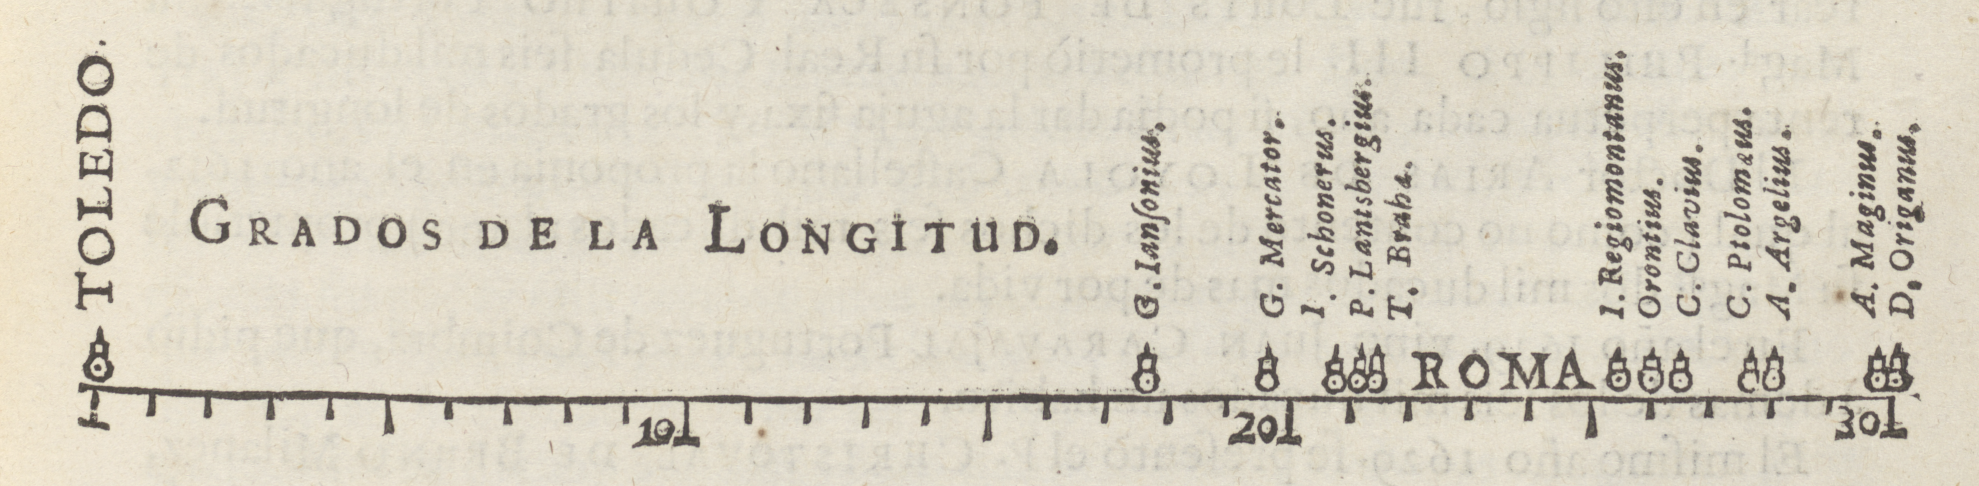
\includegraphics[width=\textheight]{florent_van_langren.png}}
    \only<2>{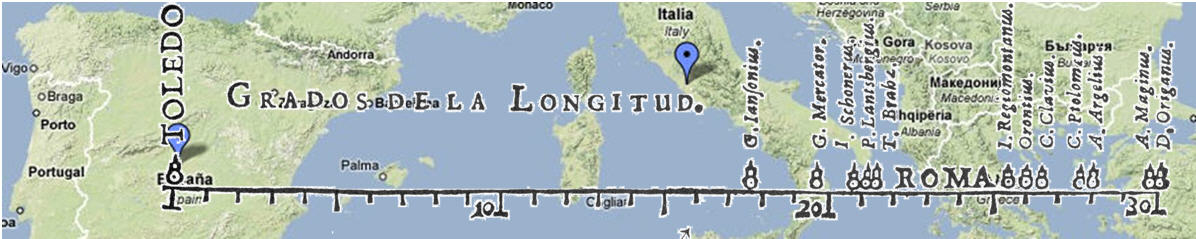
\includegraphics[width=\textheight]{florent_van_langren_overlay.jpg}}
}

%%%%%%%%%%%%%%%%%%%%%%%%%%%%%%%%%%%%%%%%%%%%%%%%%%%%%%%%%%%%%%%%%%
\frame{
\centering
\only<1>{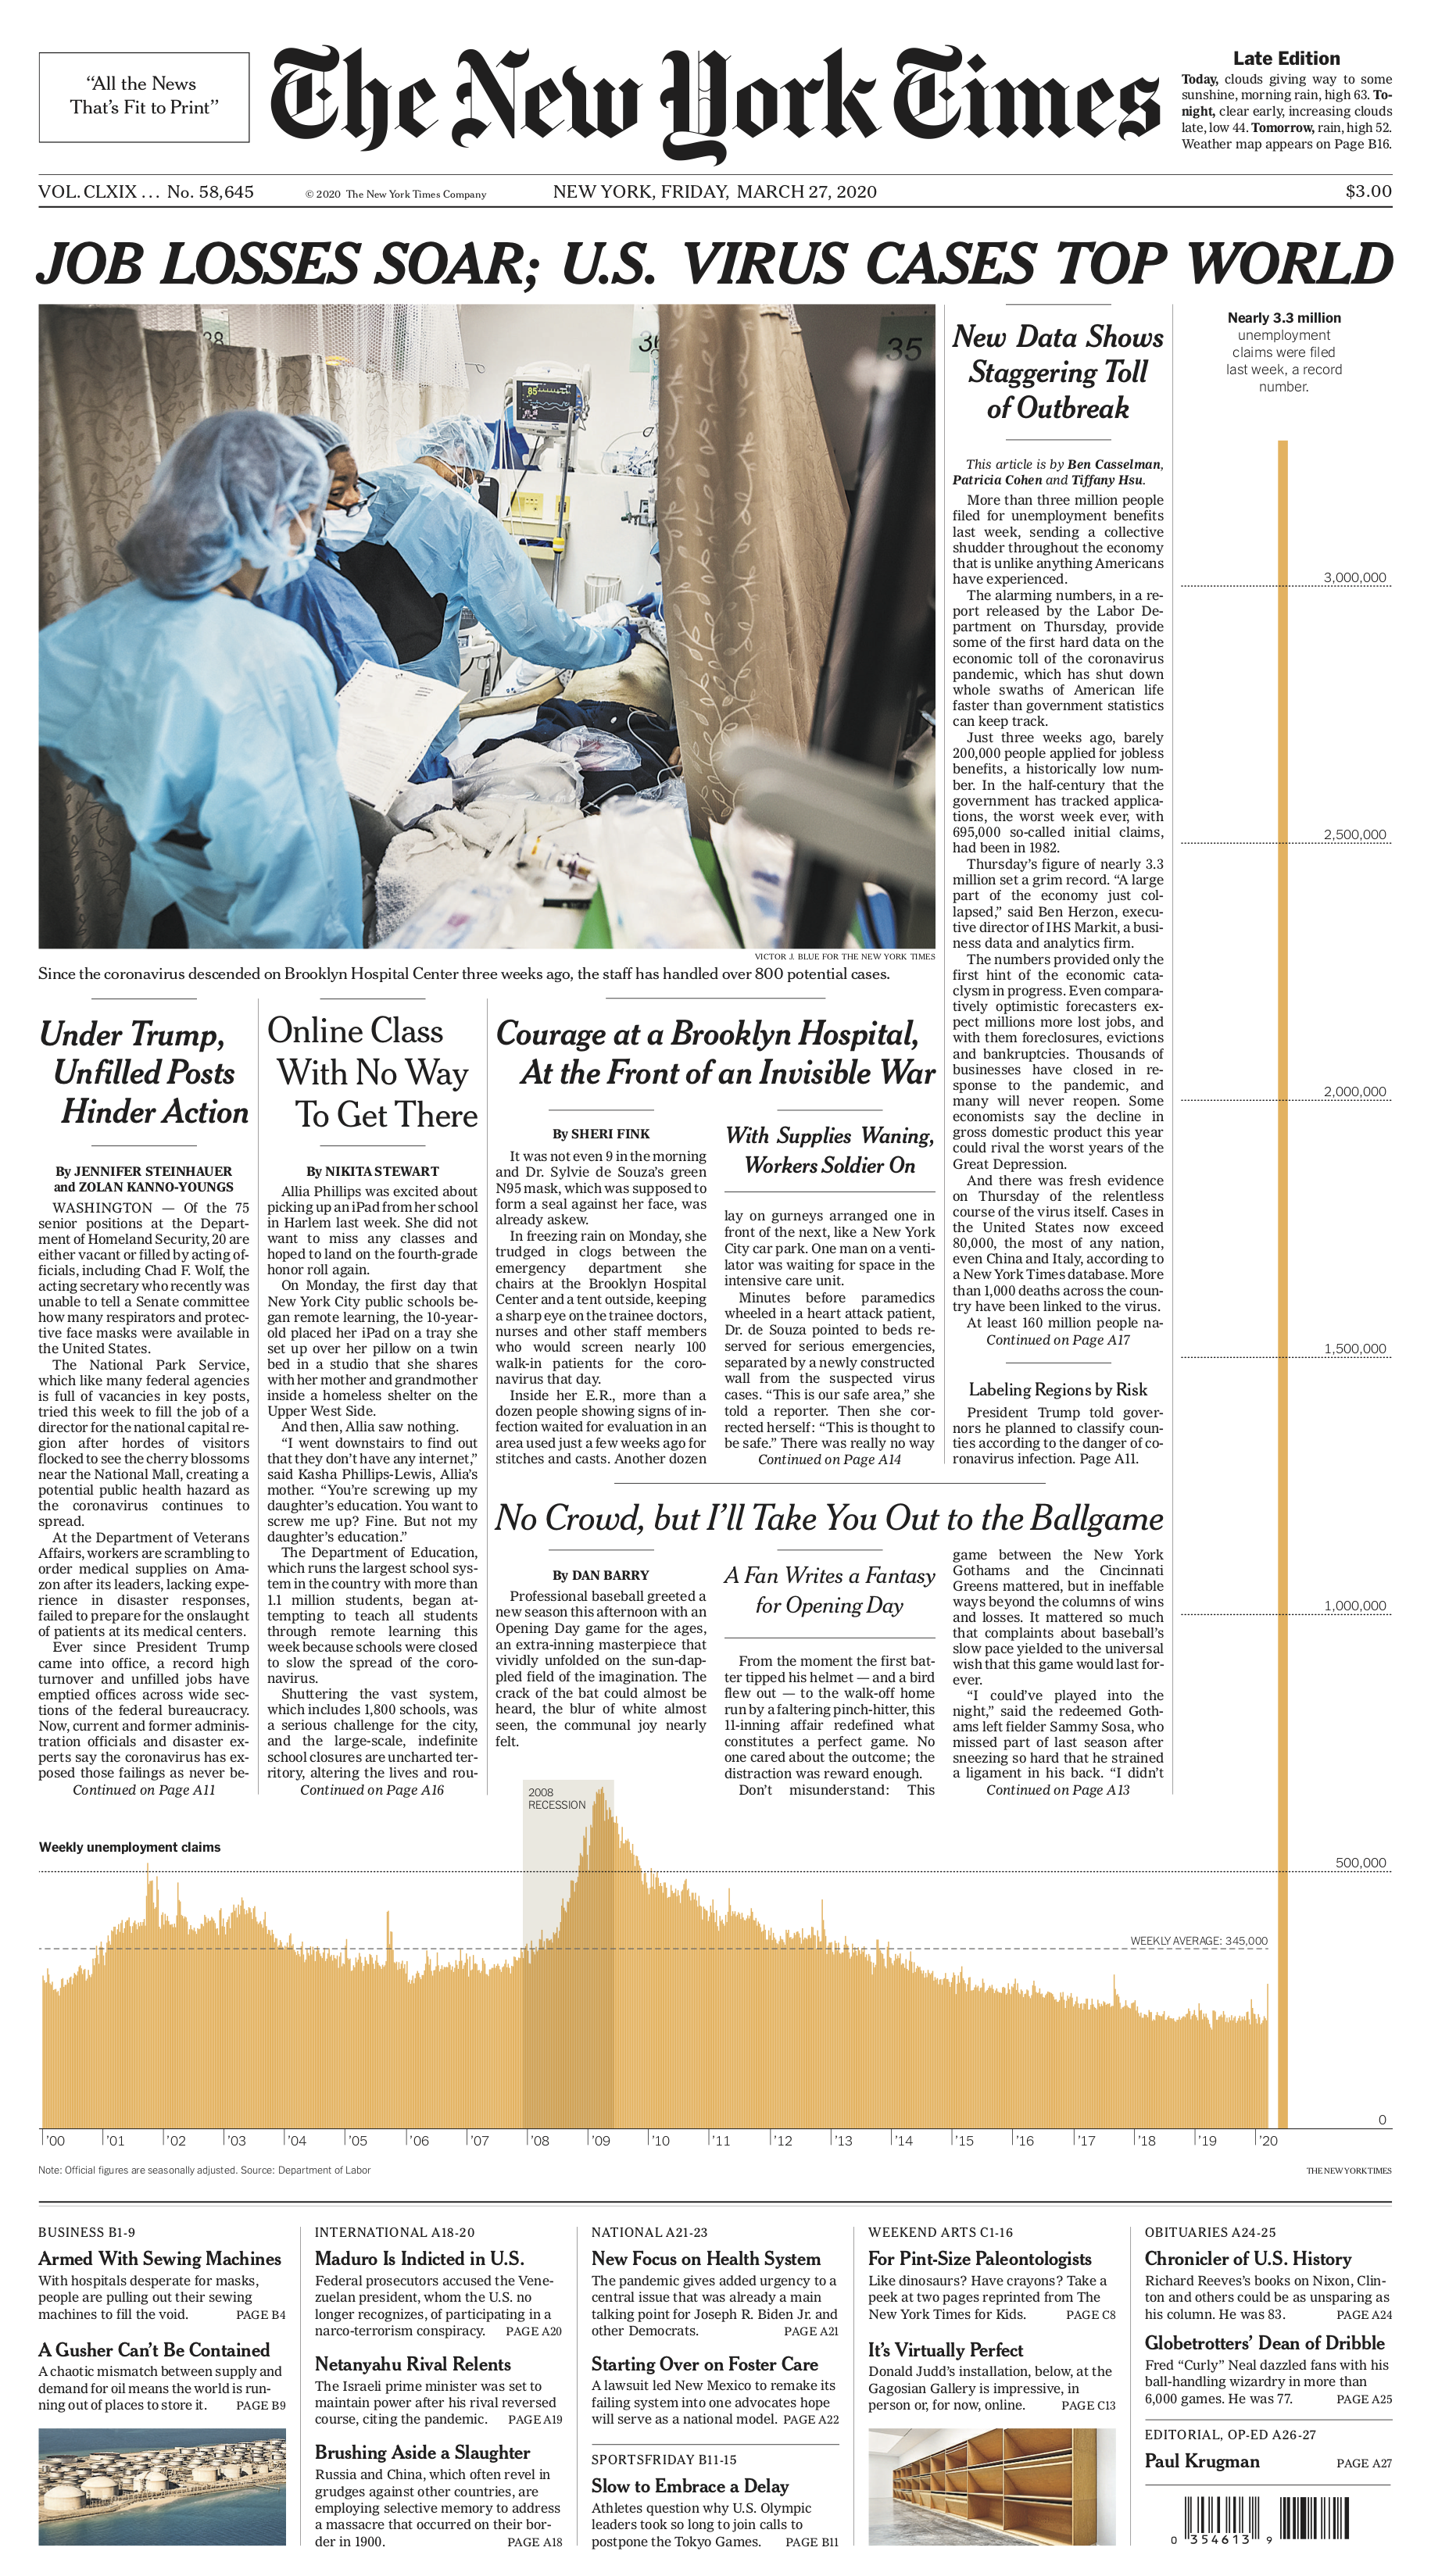
\includegraphics[height=.9\textheight]{nyt_unemp.png}}
\only<2>{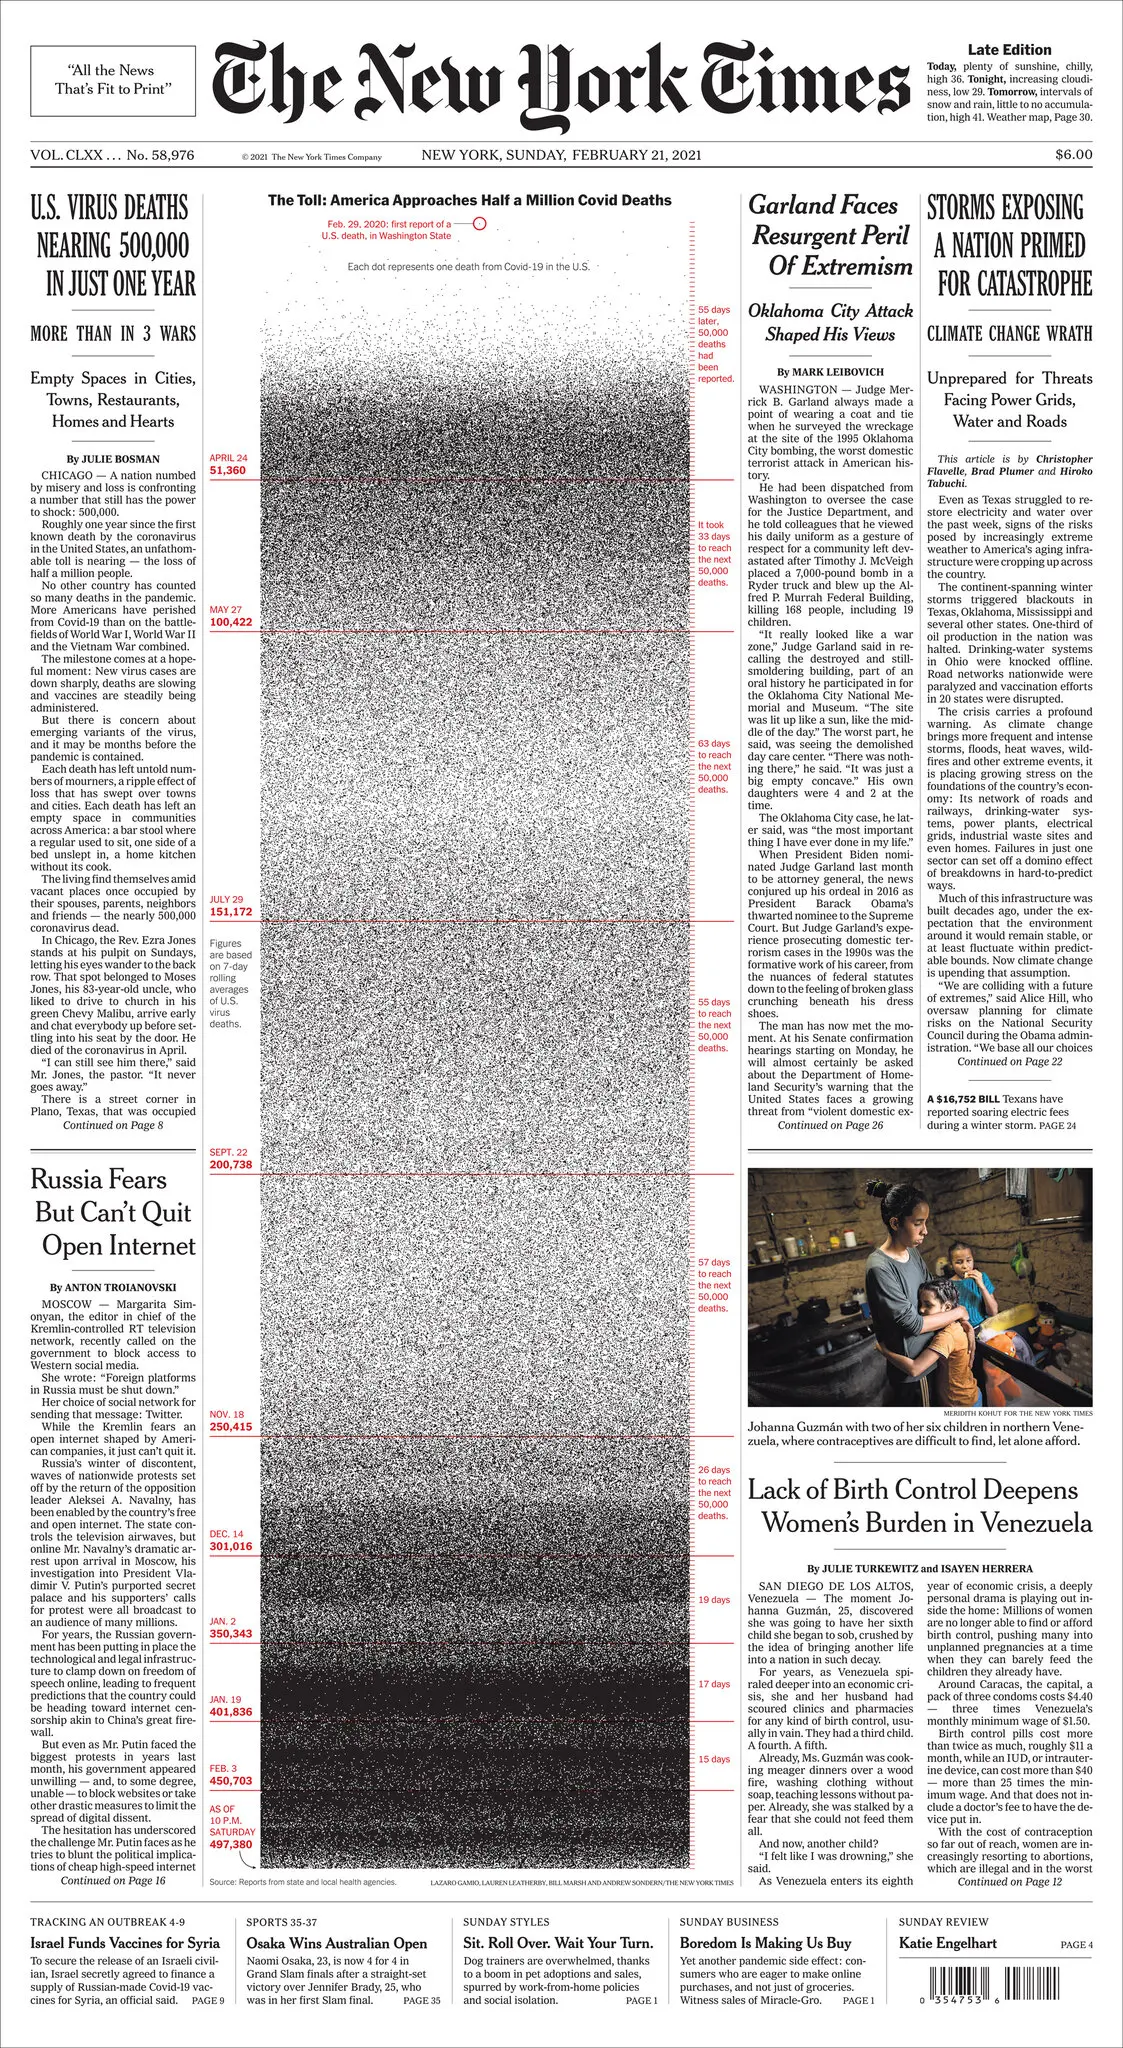
\includegraphics[height=.9\textheight]{nyt_500k.png}}
\only<3>{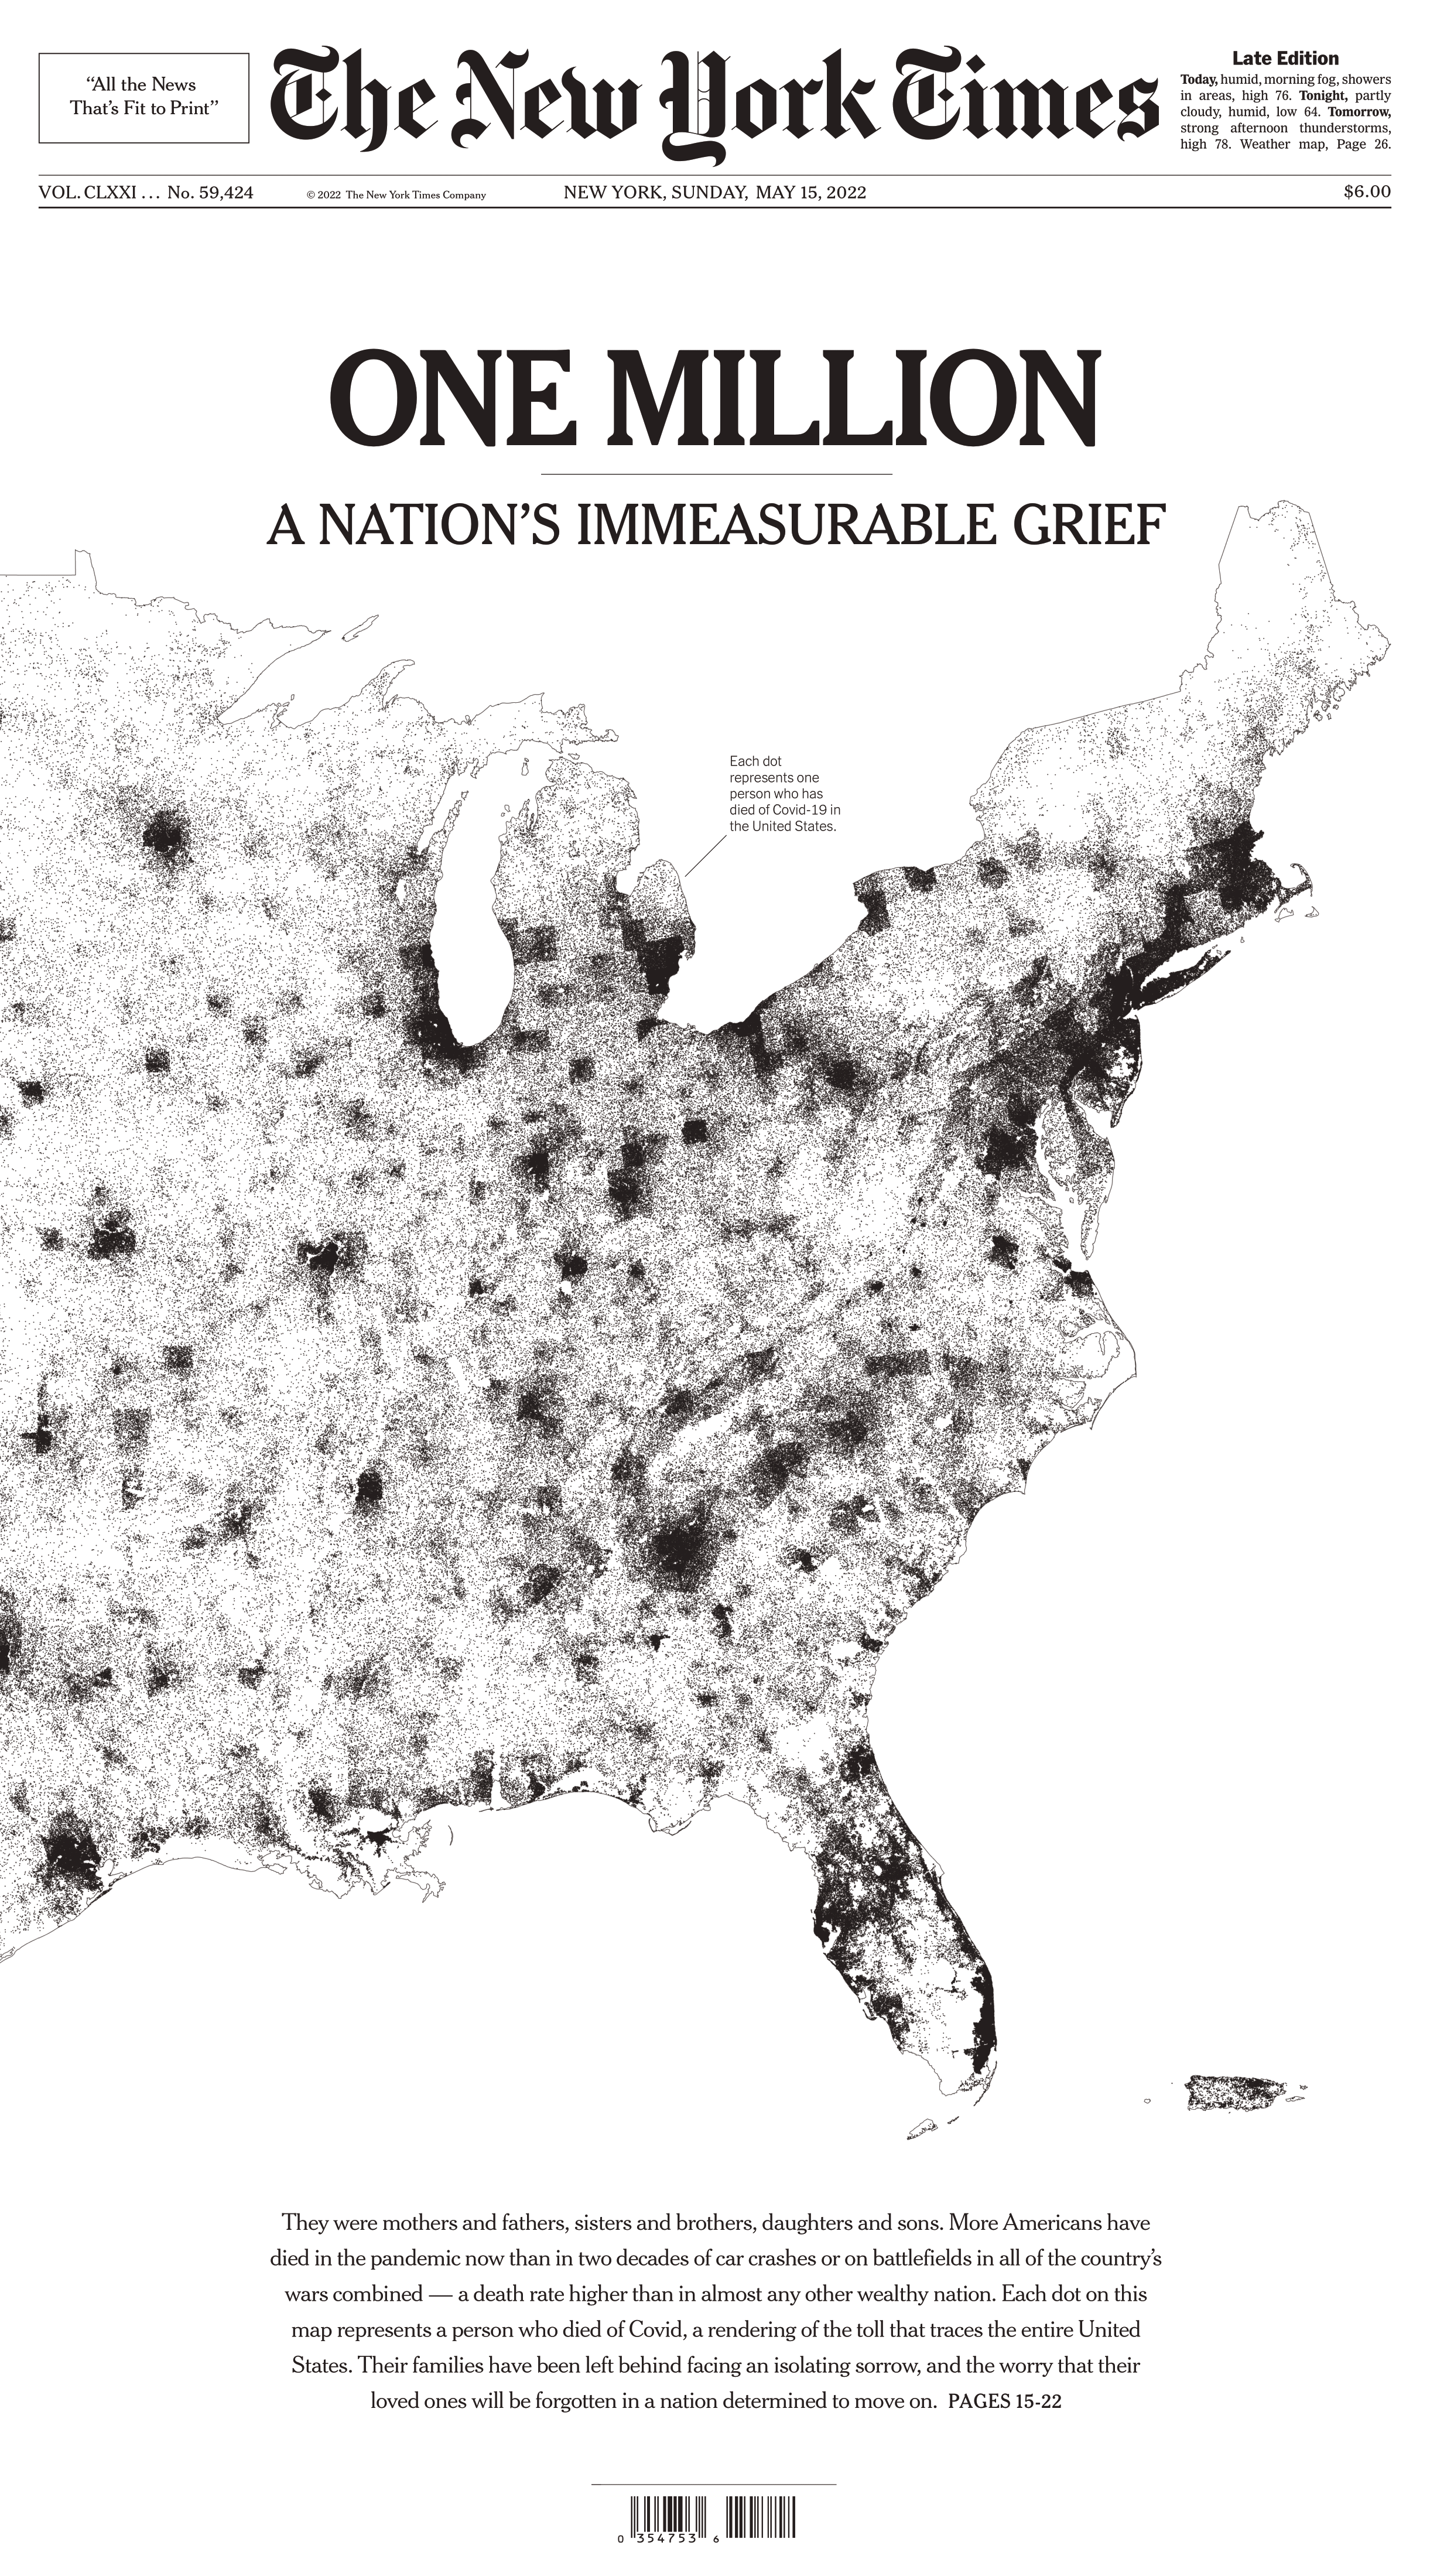
\includegraphics[height=.9\textheight]{nyt_one_million.png}}
\only<4>{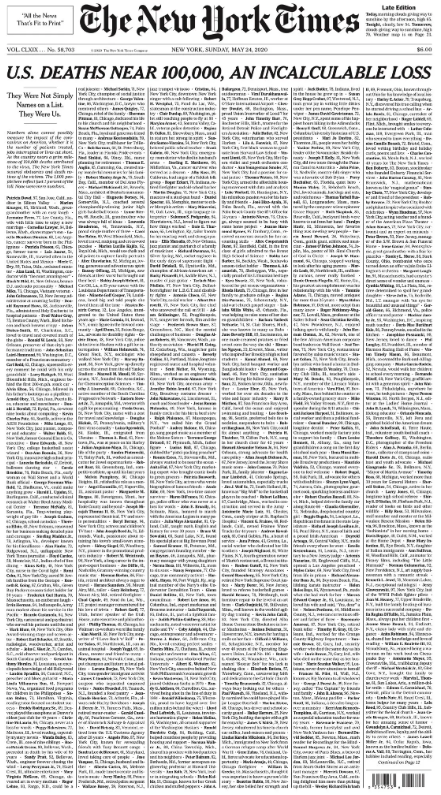
\includegraphics[height=.9\textheight]{nyt_incalculable_loss.png}}
\only<5>{
    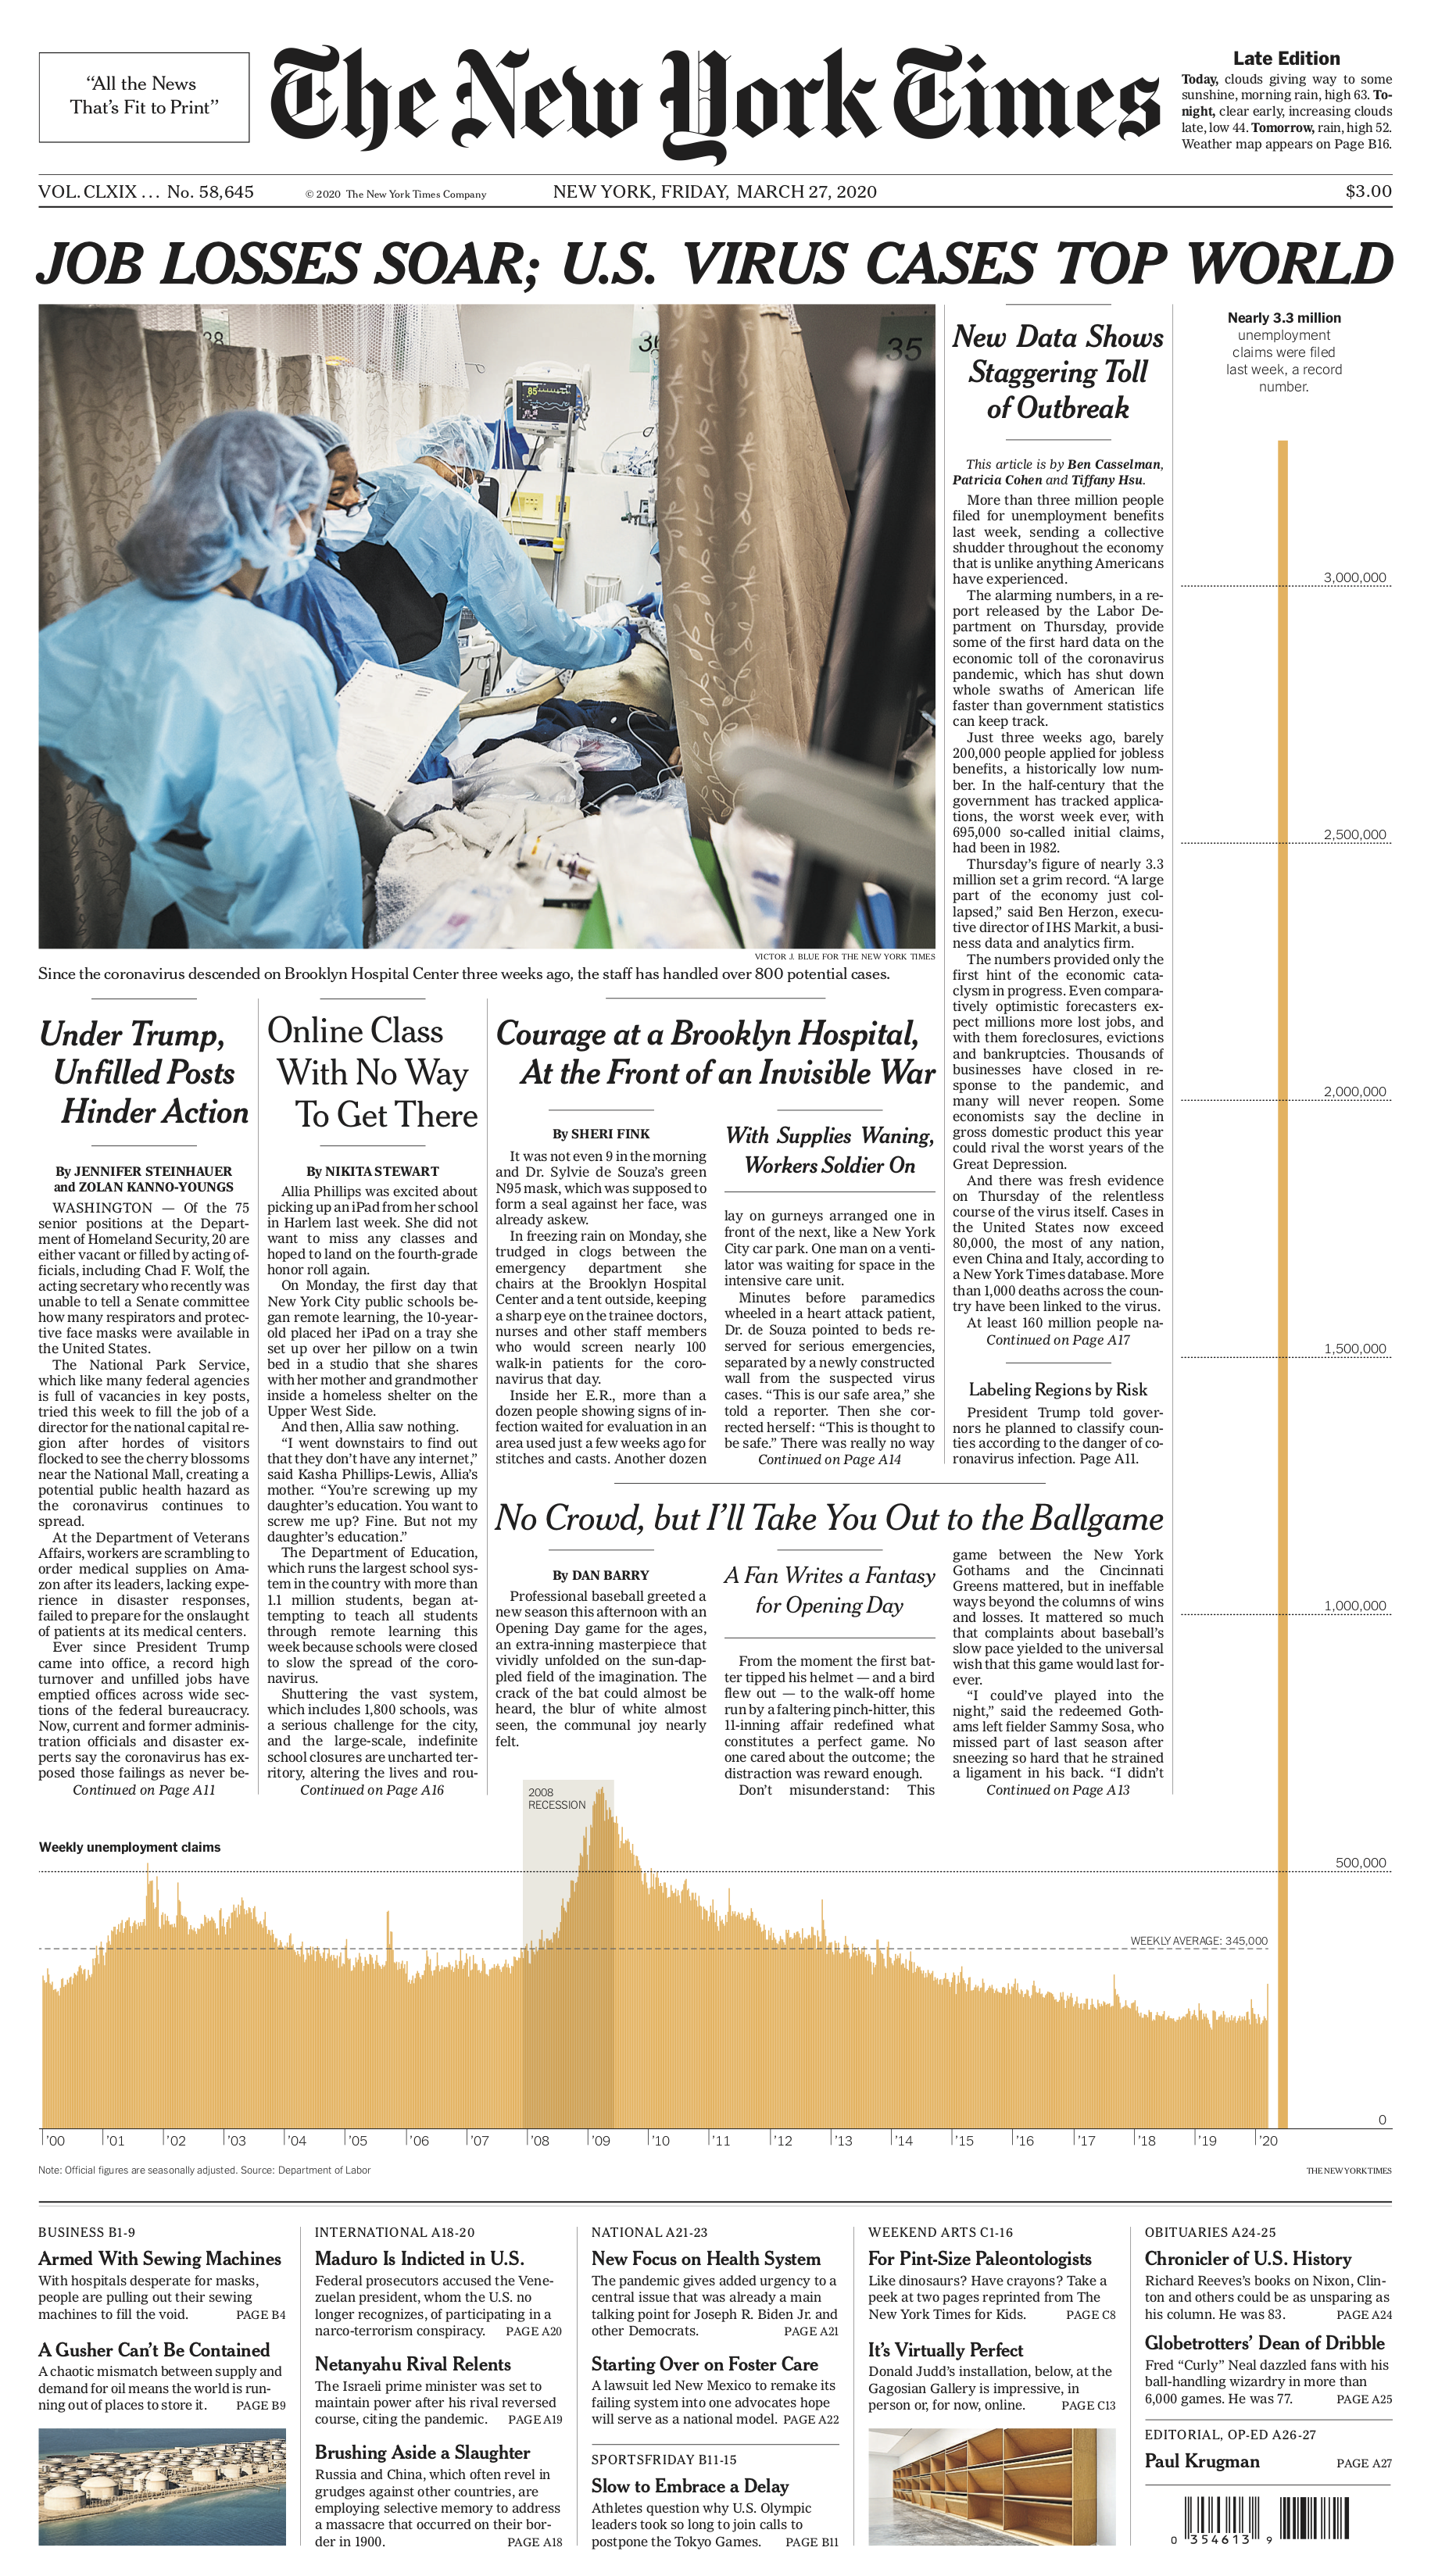
\includegraphics[width=.24\textwidth]{nyt_unemp.png} 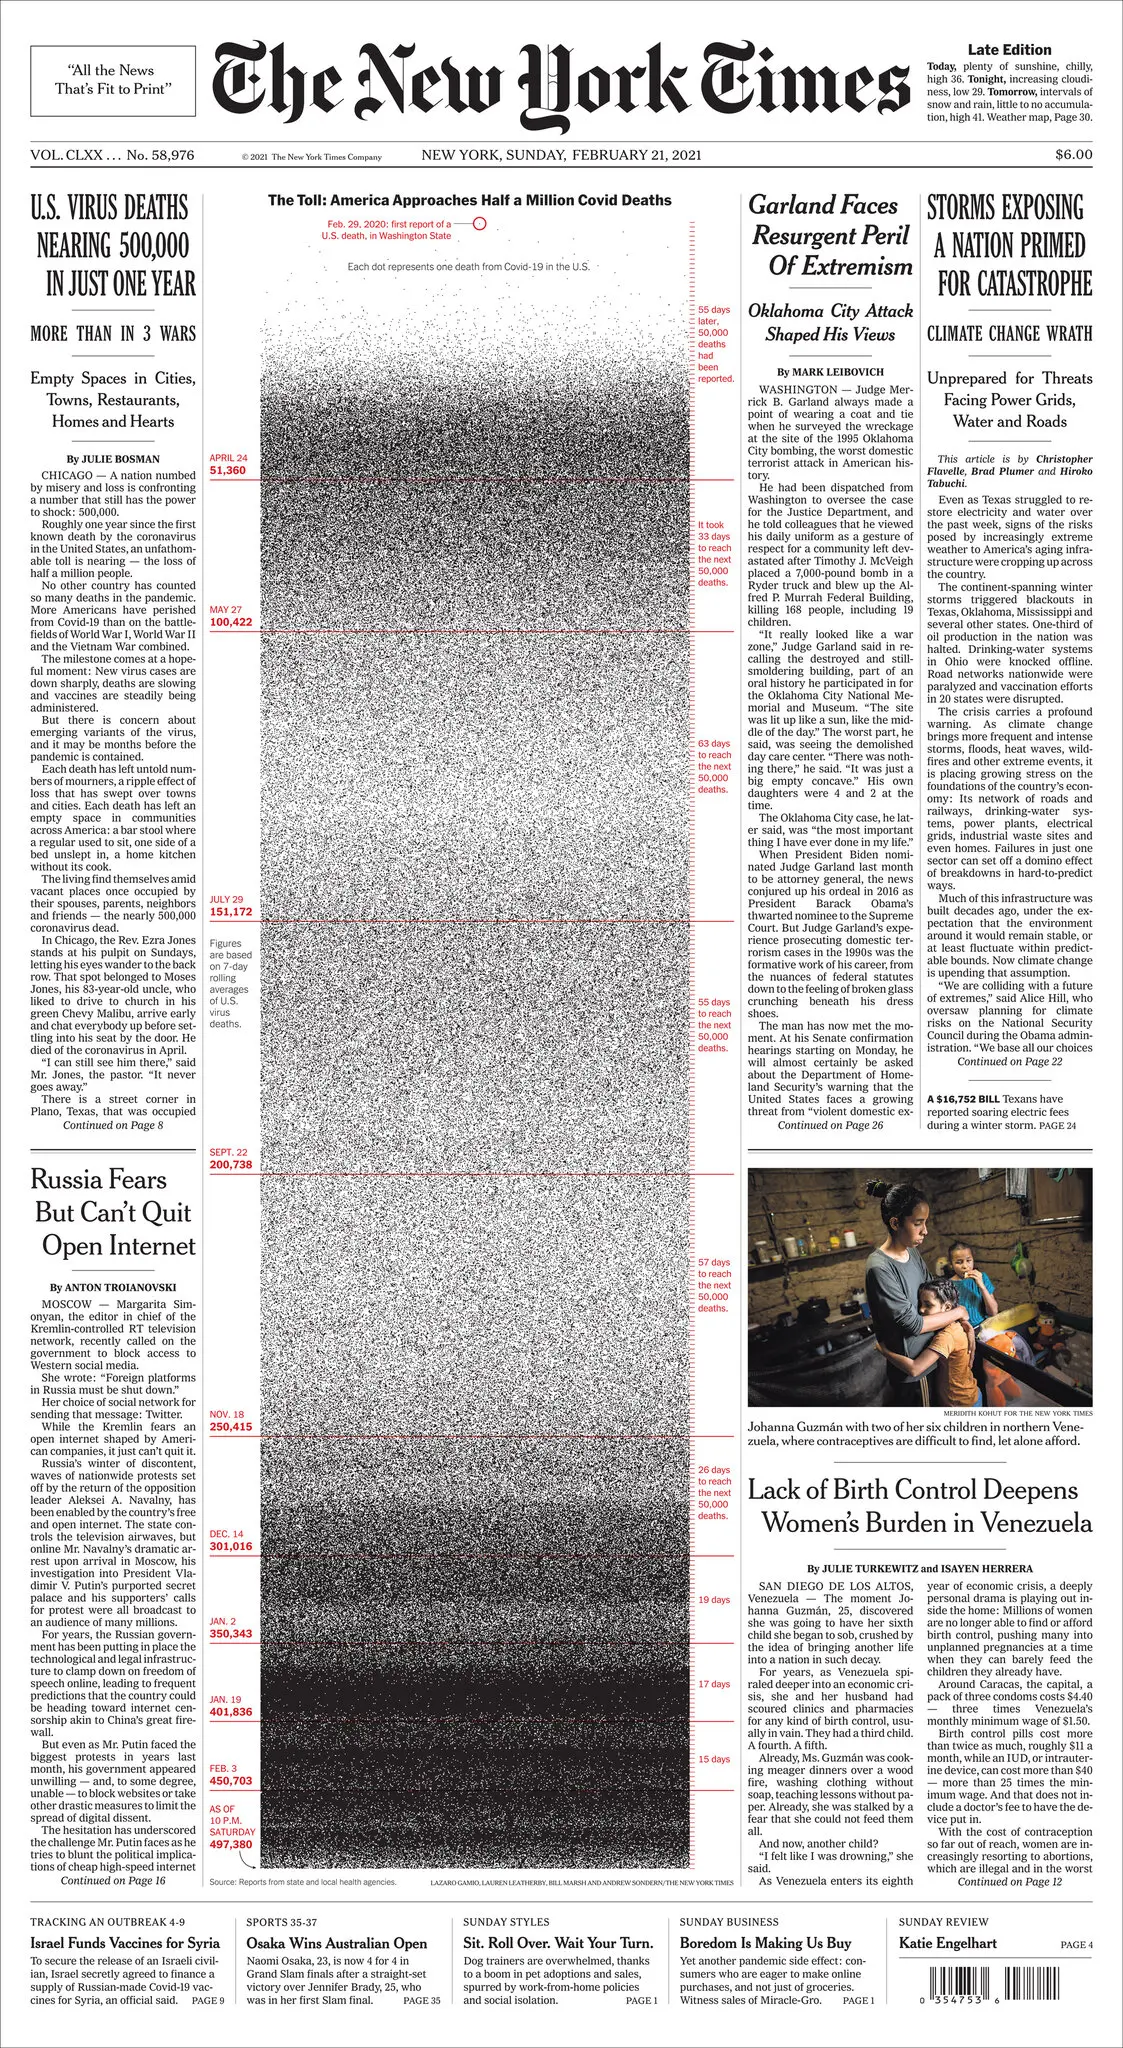
\includegraphics[width=.24\textwidth]{nyt_500k.png}
    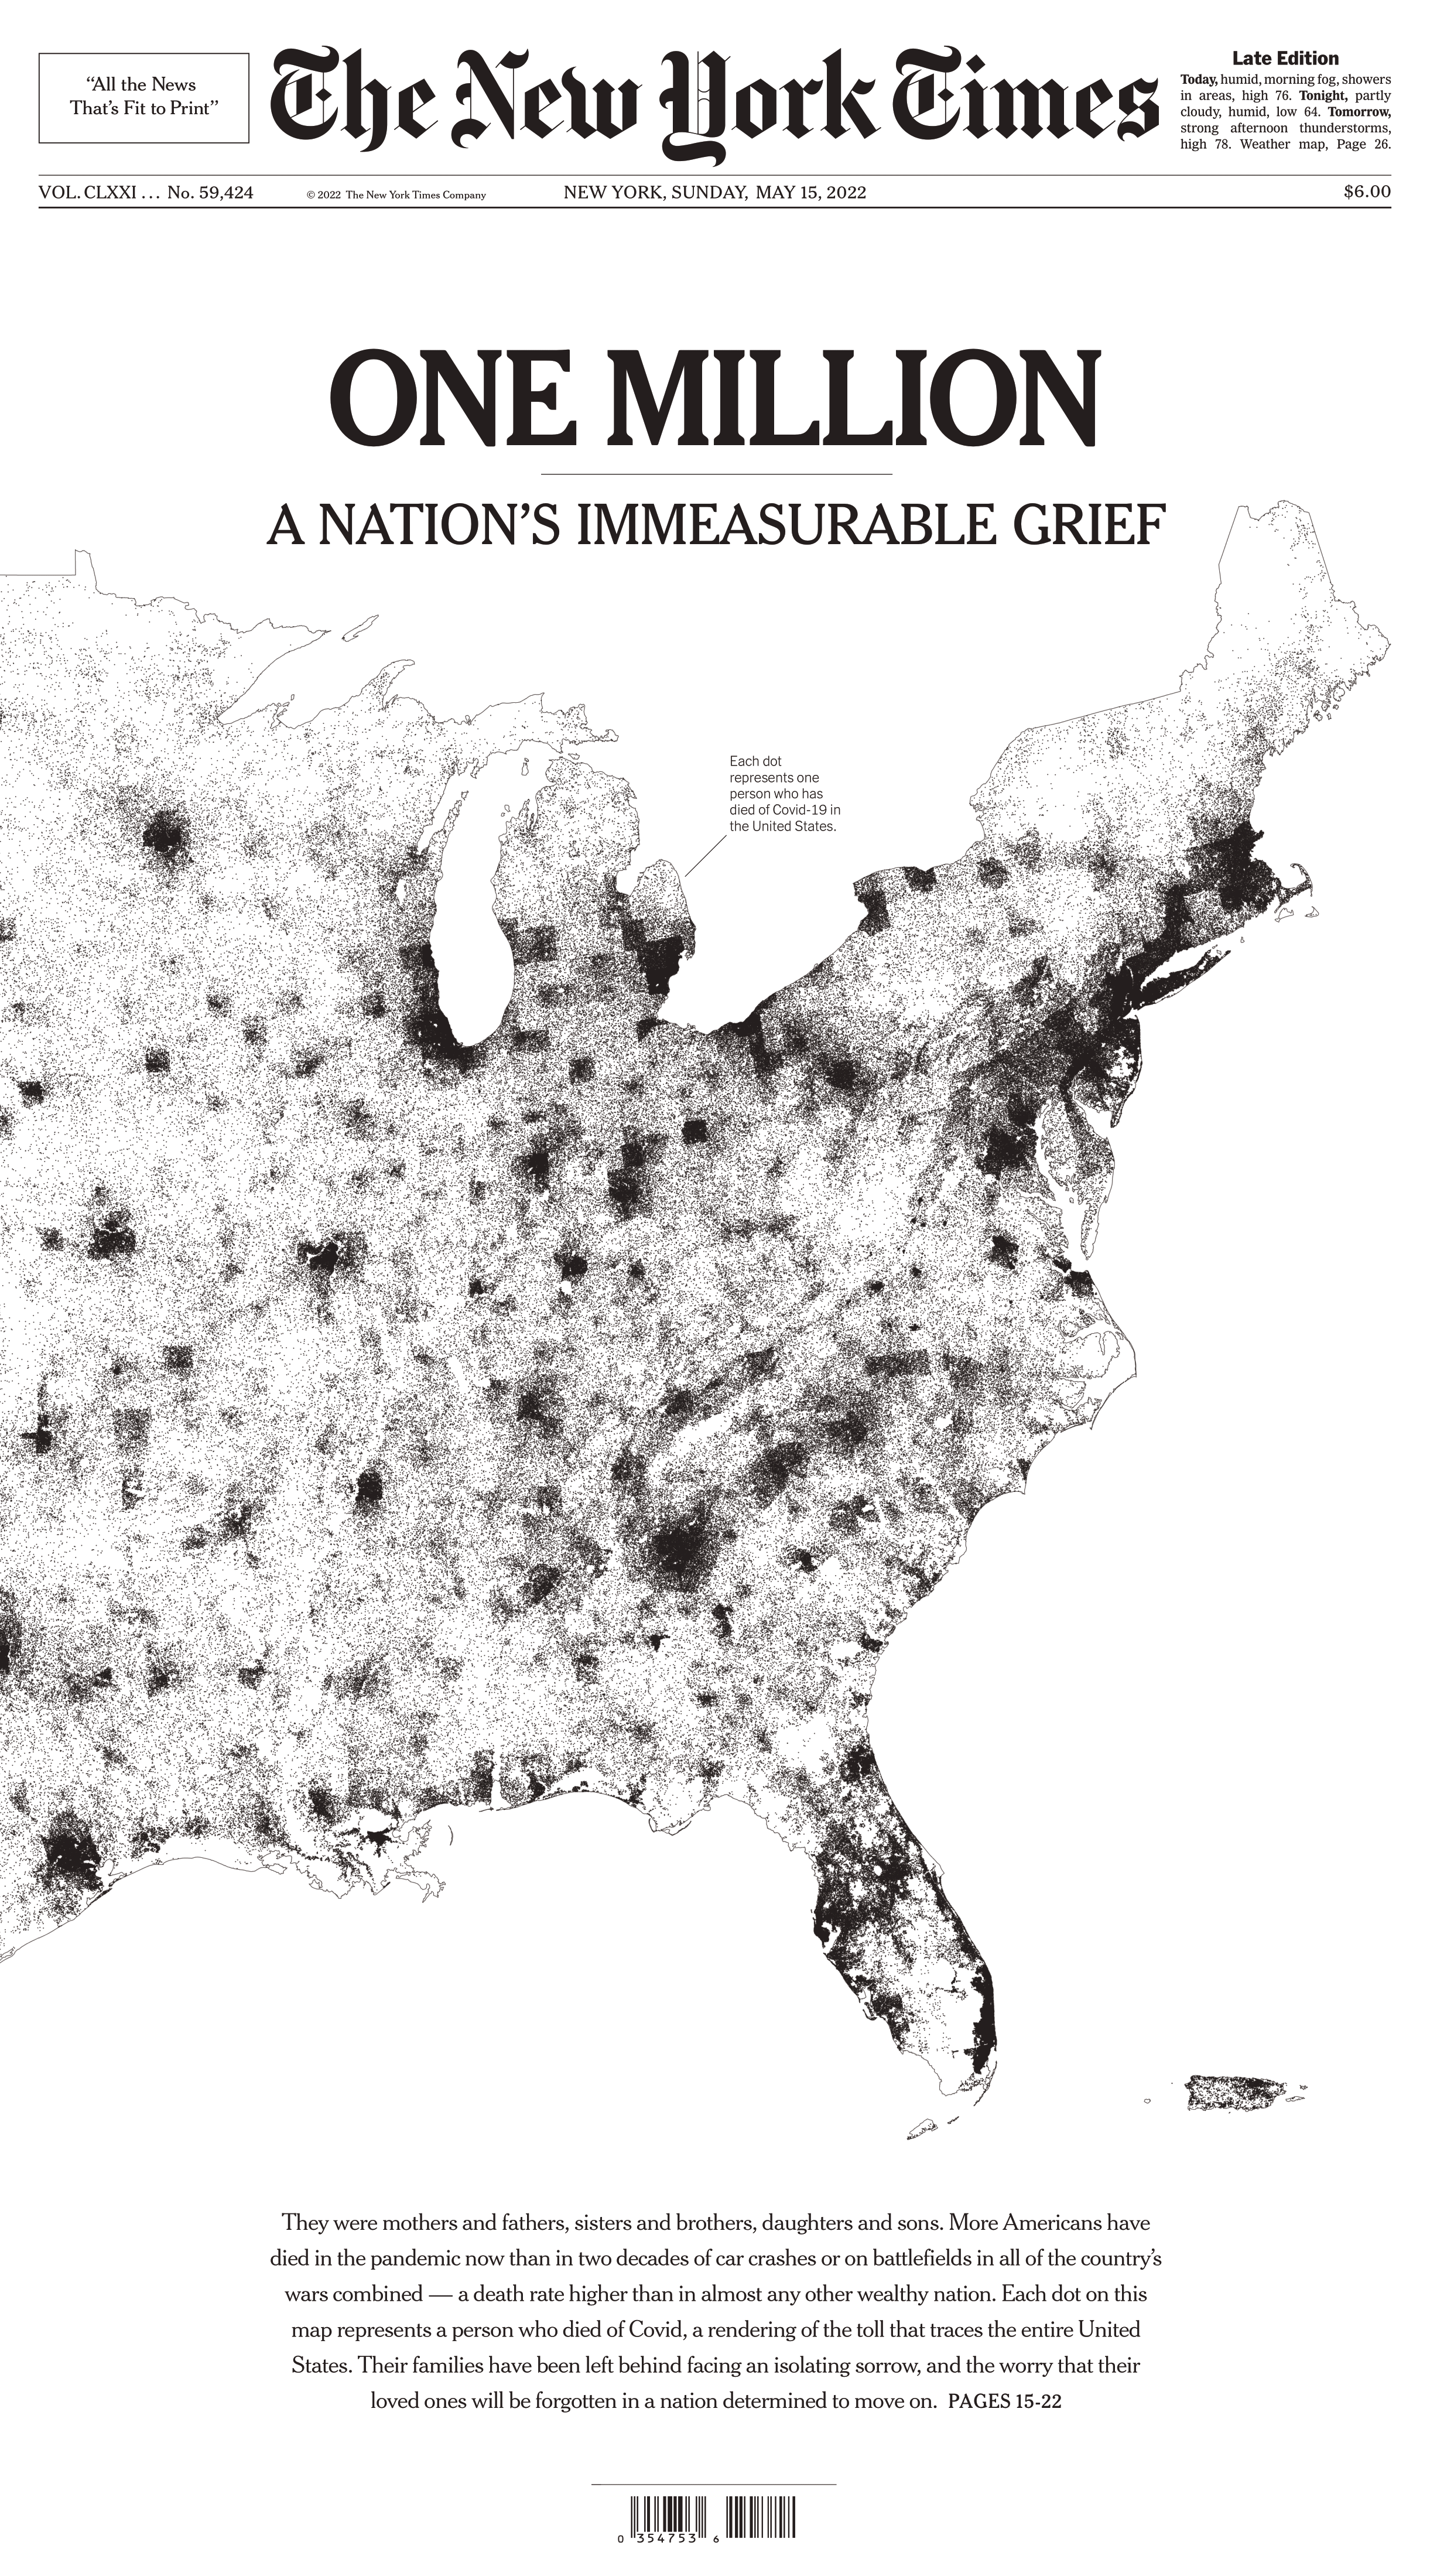
\includegraphics[width=.24\textwidth]{nyt_one_million.png} 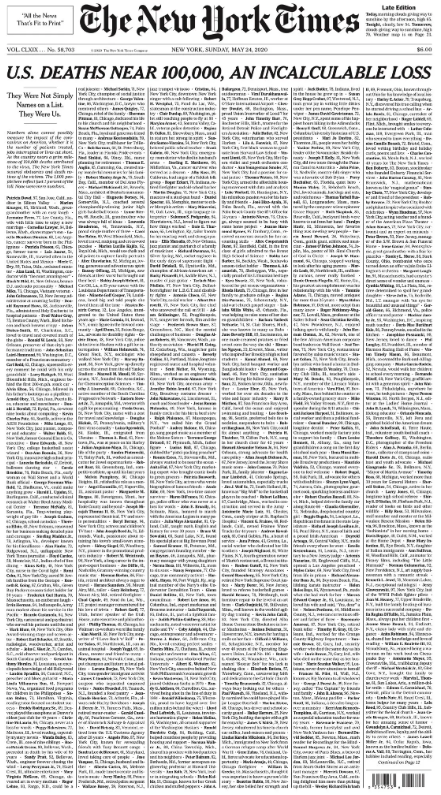
\includegraphics[width=.24\textwidth]{nyt_incalculable_loss.png}
}
}

%%%%%%%%%%%%%%%%%%%%%%%%%%%%%%%%%%%%%%%%%%%%%%%%%%%%%%%%%%%%%%%%%%
\frame{\frametitle{Early Data Visualization}
\only<1>{
    \centering
    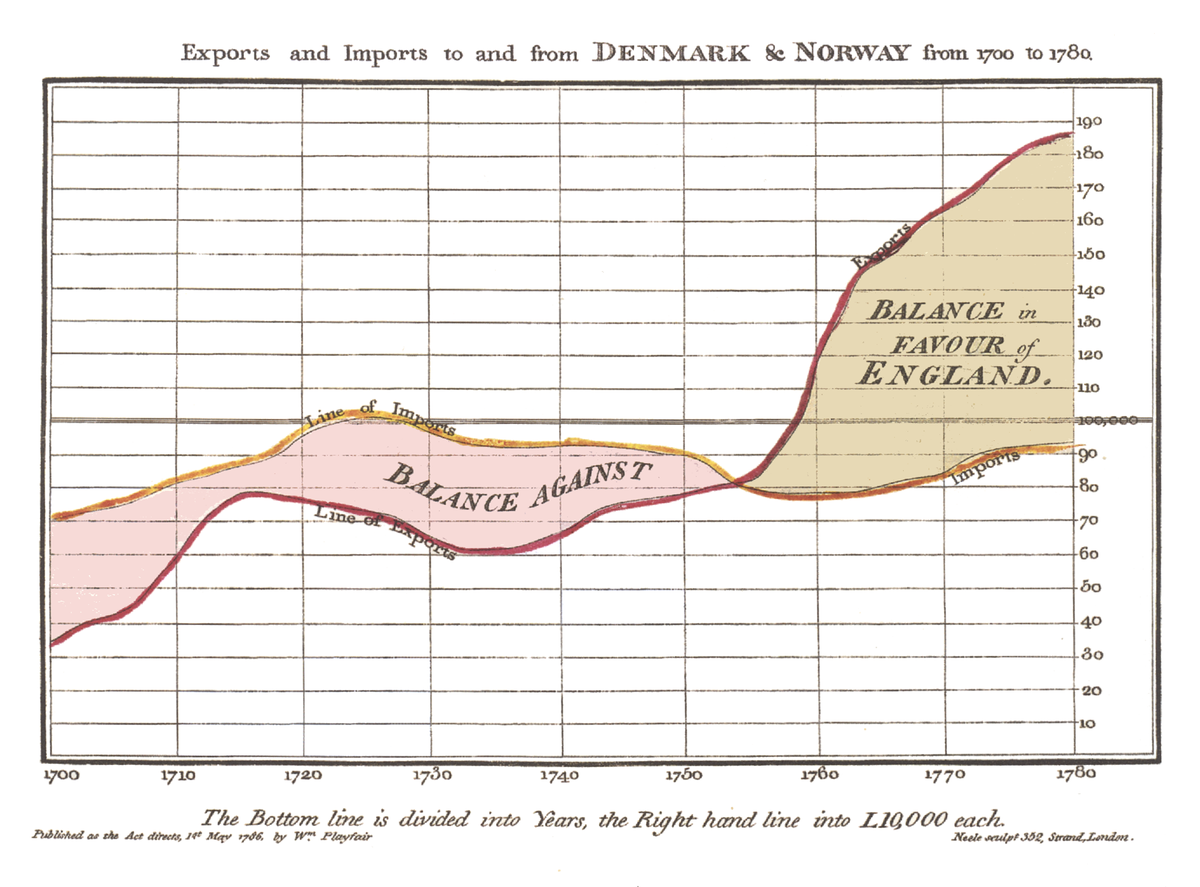
\includegraphics[height=.75\textheight]{Playfair.png}\\
    William Playfair (late 1700s)
}
\only<2>{
    \centering
    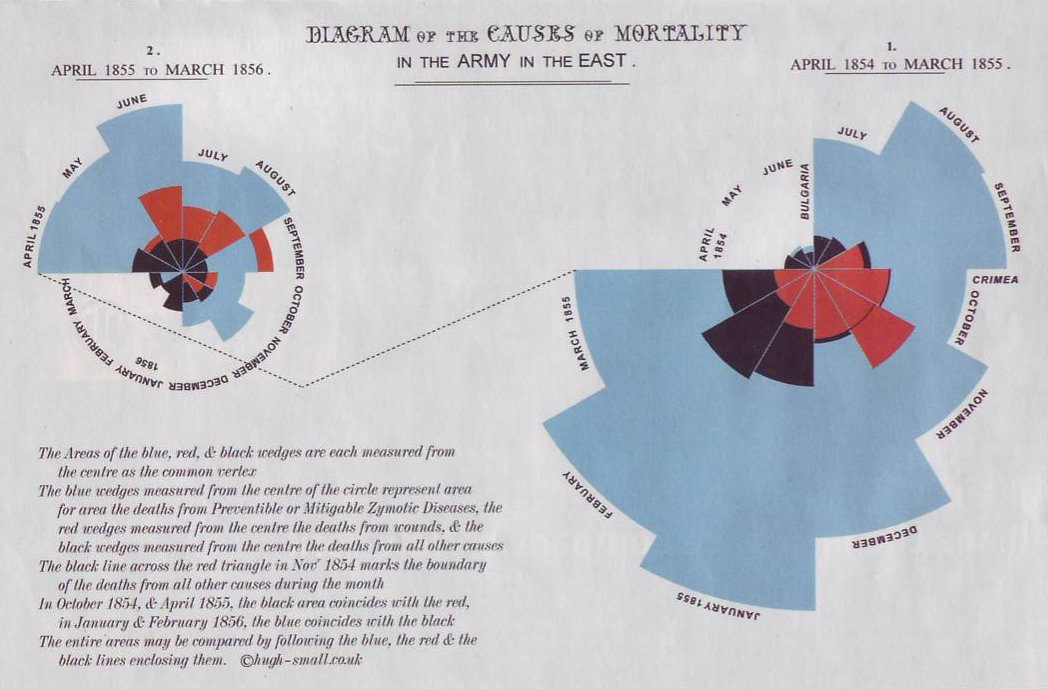
\includegraphics[height=.75\textheight]{Nightingale.jpg}\\
    Florence Nightingale (1858)
}
\only<3>{
    \centering
    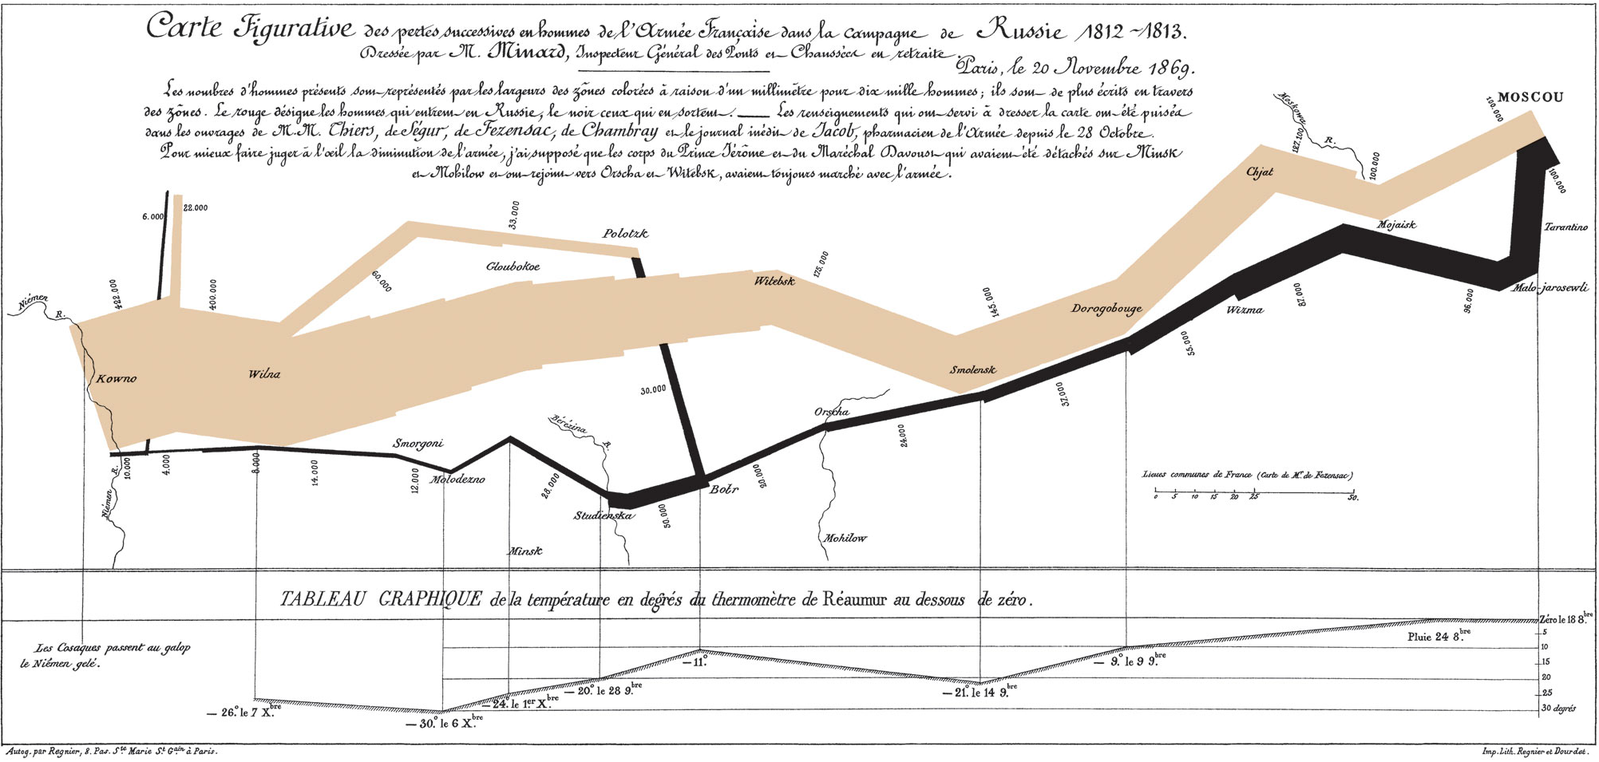
\includegraphics[width=\textwidth]{Minard.png}\\
    Charles Minard (1861)
}
}

%%%%%%%%%%%%%%%%%%%%%%%%%%%%%%%%%%%%%%%%%%%%%%%%%%%%%%%%%%%%%%%%%%

\frame{\frametitle{Edward Tufte}
\only<1-3, 8>{
    Published \textit{The Visual Display of Quantitative Information} in 1983\\
    ~\\
    \begin{enumerate}[<+(1)->]
        \item ``Above all else, show the data.''
        \item Maximize the amount of data and minimize the amount of ink
        \item<8> Opponent of unnecessary graphical design (``chartjunk'')
    \end{enumerate}
}

\only<4>{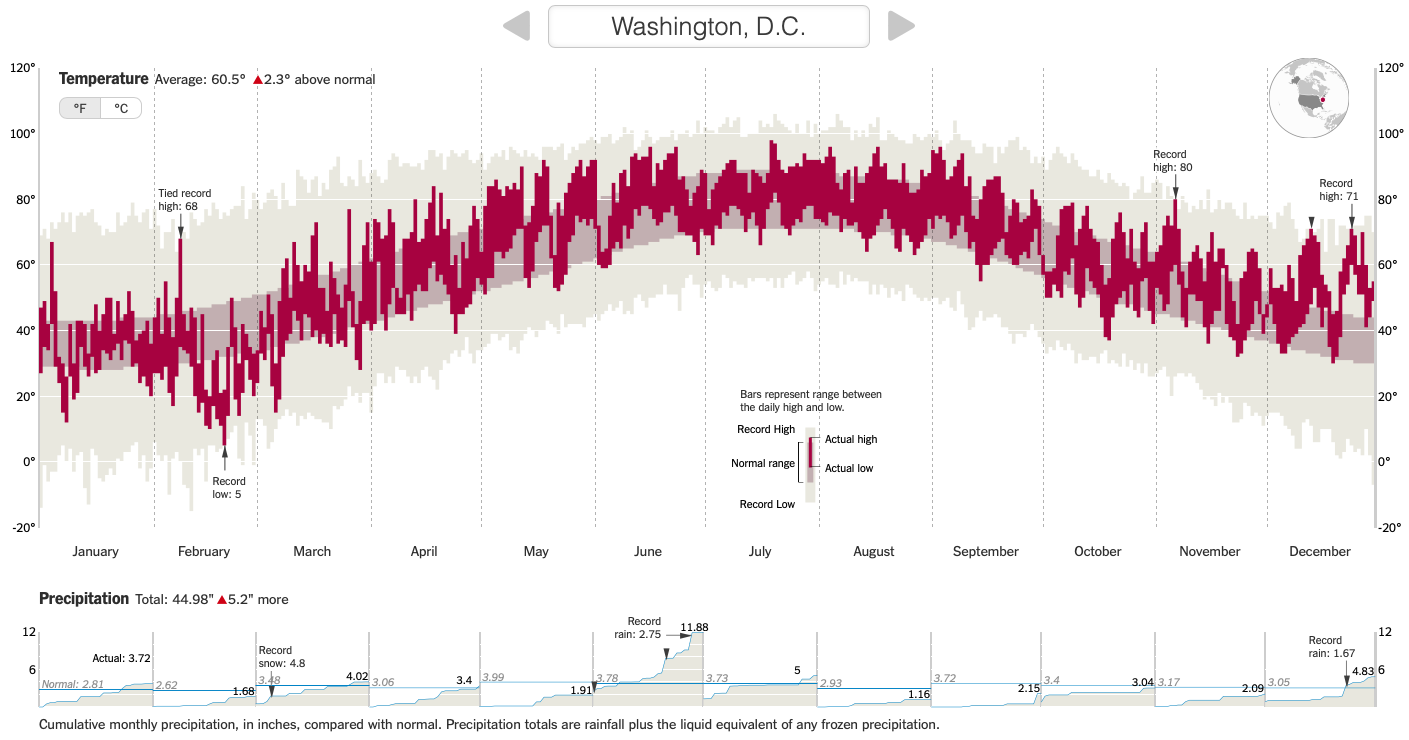
\includegraphics[width=\textwidth]{nyt_modern.png}}
\only<5>{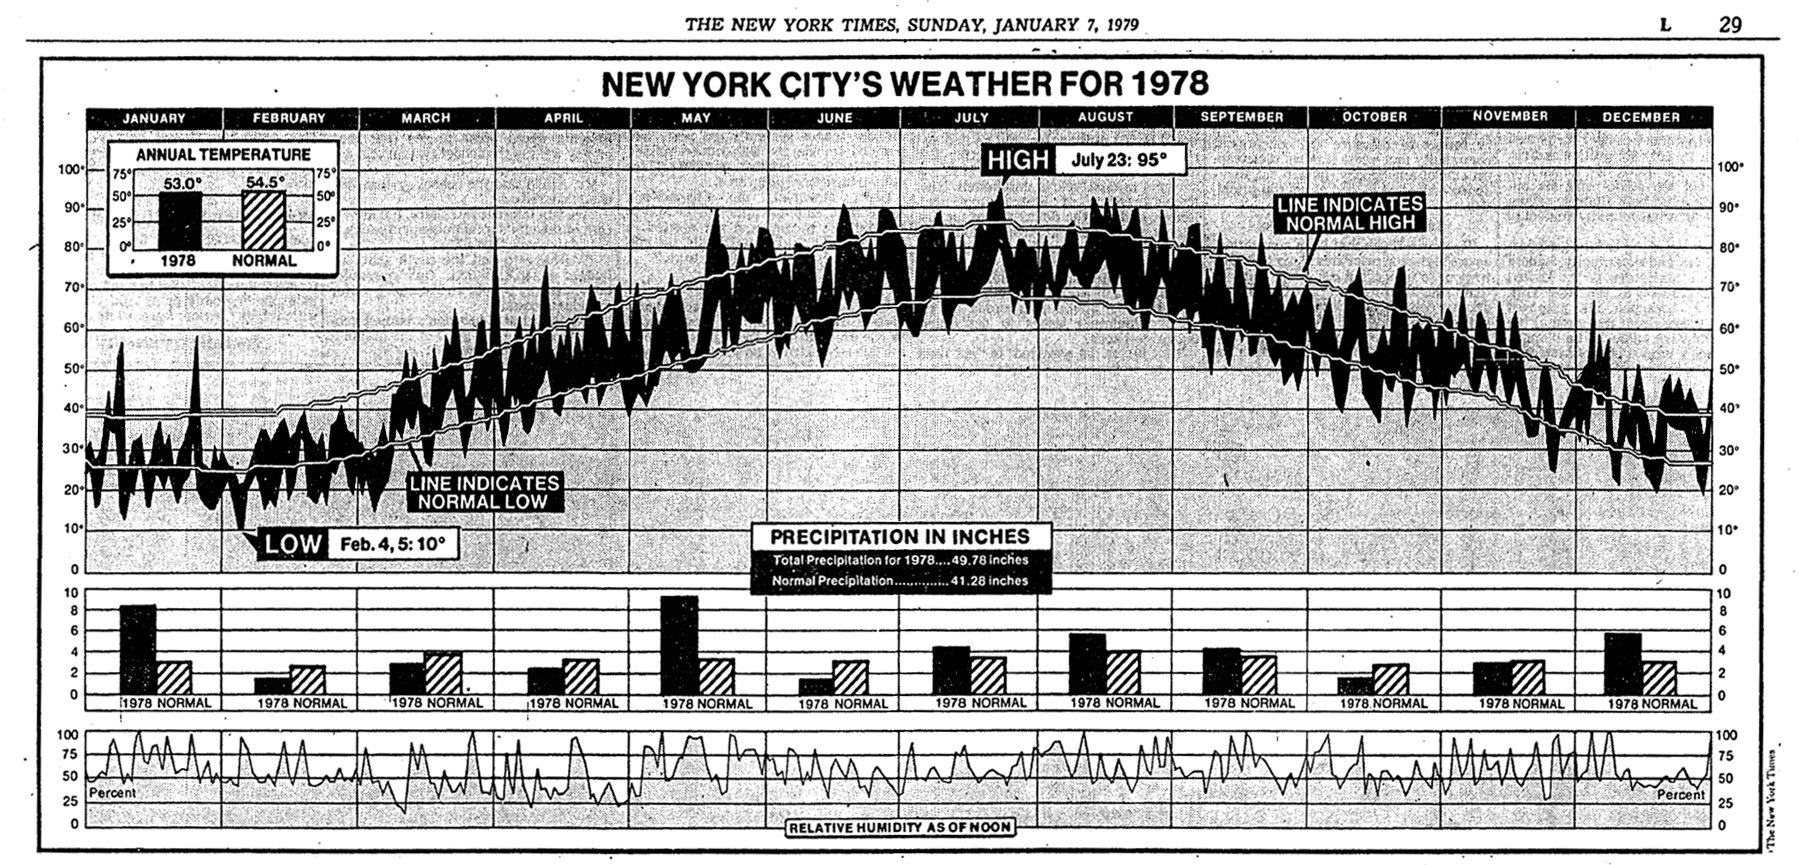
\includegraphics[width=\textwidth]{nyt_weather_1979.jpg}}
\only<6>{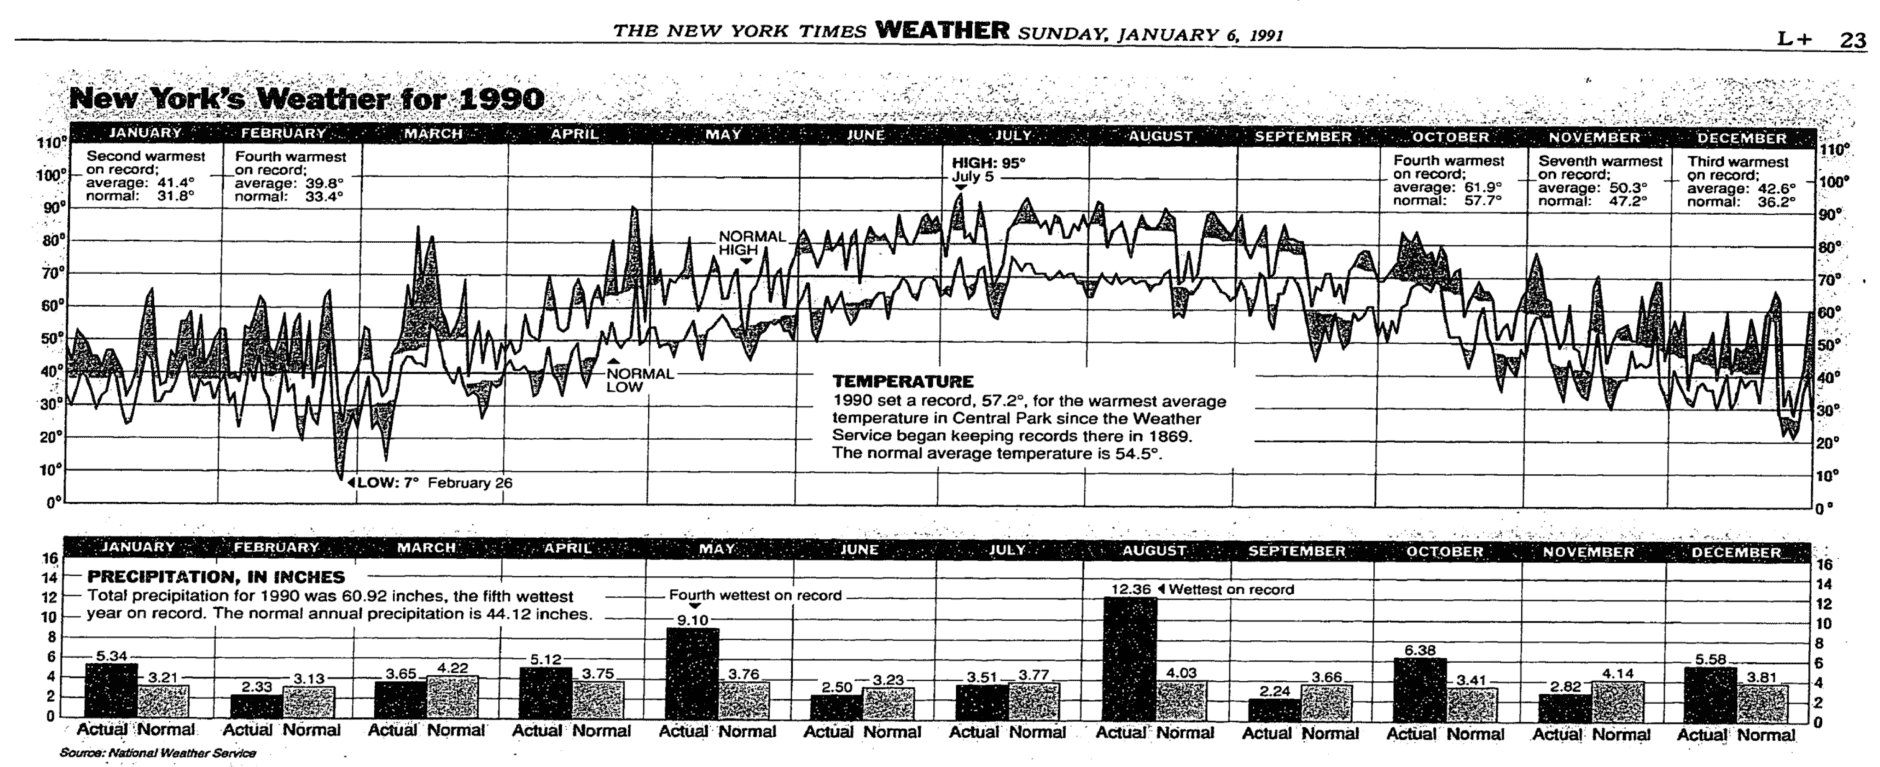
\includegraphics[width=\textwidth]{nyt_weather_1991.png}}
\only<7>{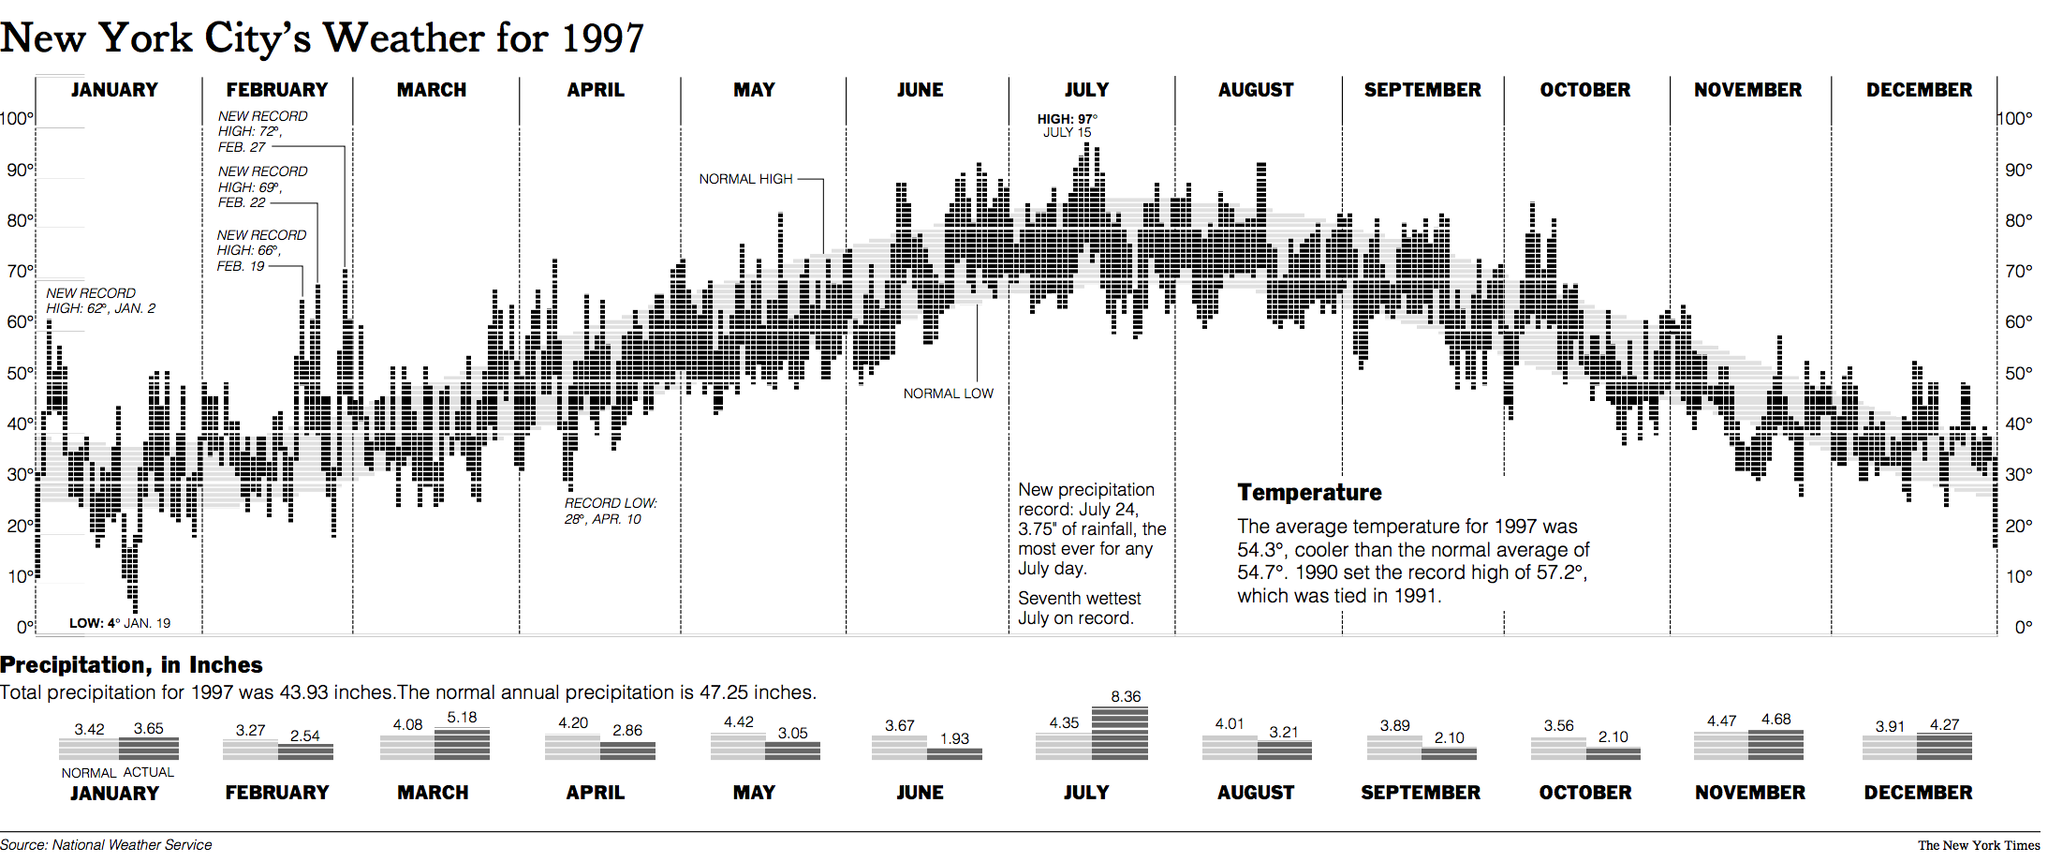
\includegraphics[width=\textwidth]{nyt_weather_1998.png}}
\only<9>{\centering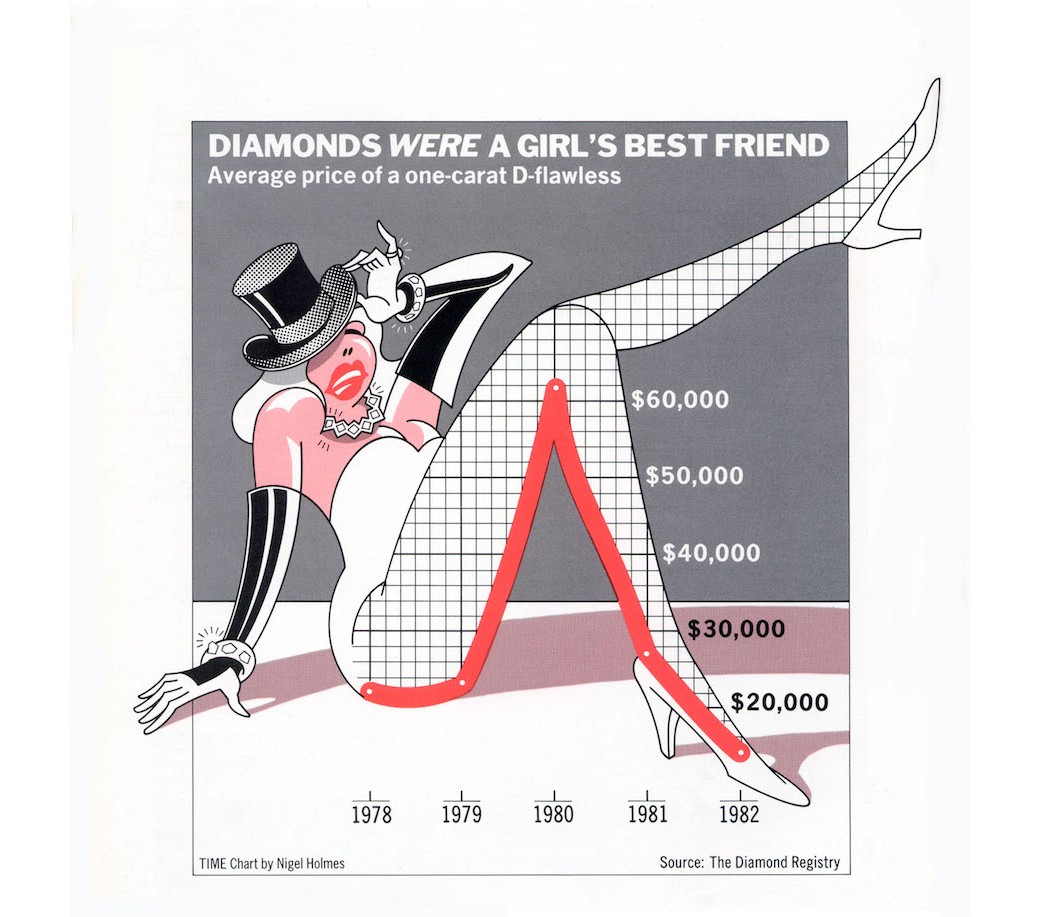
\includegraphics[height=.8\textheight]{holmes.jpg}}
\only<10>{\centering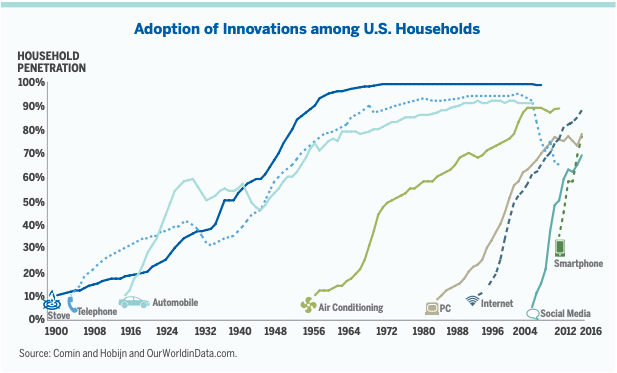
\includegraphics[width=.9\textwidth]{tech_adoption.png}\\\scriptsize Source: Fred Alger \& Co., Inc.}
}

%%%%%%%%%%%%%%%%%%%%%%%%%%%%%%%%%%%%%%%%%%%%%%%%%%%%%%%%%%%%%%%%%%
\frame{\frametitle{Engineers vs. Designers}
\only<1>{
    \begin{center}
    \begin{tabularx}{.9\textwidth}{|*{2}{X|}}
    \hline
    \textbf{Engineers} & \textbf{Designers} \\
    \hline
    $\bullet$ Simplicity of design & $\bullet$ Artistic expression \\
    $\bullet$ Maximize the data & $\bullet$ Express only a few ideas \\
    $\bullet$ Assumes the viewer is alert and interested & $\bullet$ Assumes the viewer is inattentive \\
    $\bullet$ Form follows function & $\bullet$ Many forms can convey the same data \\
    \hline
    \end{tabularx}
    \end{center}
}

\only<2>{\centering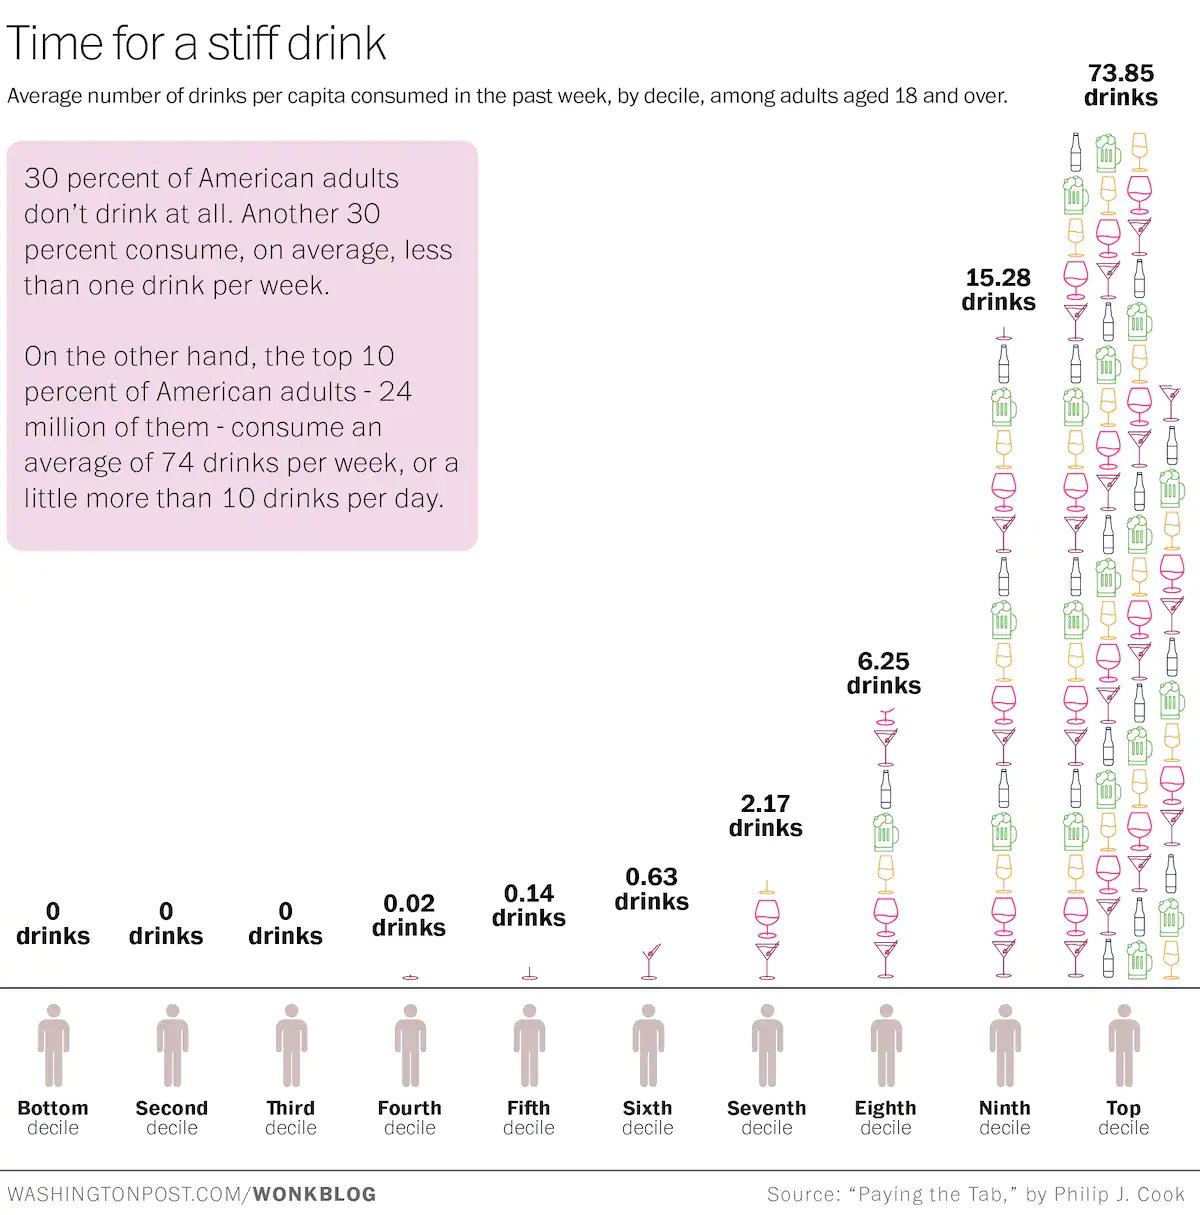
\includegraphics[height=.8\textheight]{us_drinking.jpg}}
}

%%%%%%%%%%%%%%%%%%%%%%%%%%%%%%%%%%%%%%%%%%%%%%%%%%%%%%%%%%%%%%%%%%
\frame{\frametitle{Science of Data Visualization}
\only<1>{
    \huge
    \begin{center}
    Sight \MVRightarrow{} Perception \MVRightarrow{} Cognition
    \end{center}
}

\only<2-4>{
    {\Large \textbf{Sight}}
    \begin{itemize}[<+(1)->]
        \item The eyes send small snapshots of high-resolution focus to the brain, which puts the snapshots together into a single image
        \item The order in which the eyes take these snapshots is not random -- it is optimized through evolution (i.e., moving objects, pure colors get attention first)
        \item When we design data visualization, the first question to ask is: \textbf{where do my eyes go first?}
    \end{itemize}
}

\only<5-6,17>{
    {\Large \textbf{Perception}}
    \begin{itemize}[<+(4)->]
        \item Known as ``preattentive features''
        \item The brain is optimized to quickly identify contrasts in color and recognize groups
        \item<17> After ``where do my eyes go first?'', the next question is: \textbf{what is the first idea that comes to mind?}
    \end{itemize}
}

\only<7>{\centering\large Color Contrasts\\~\\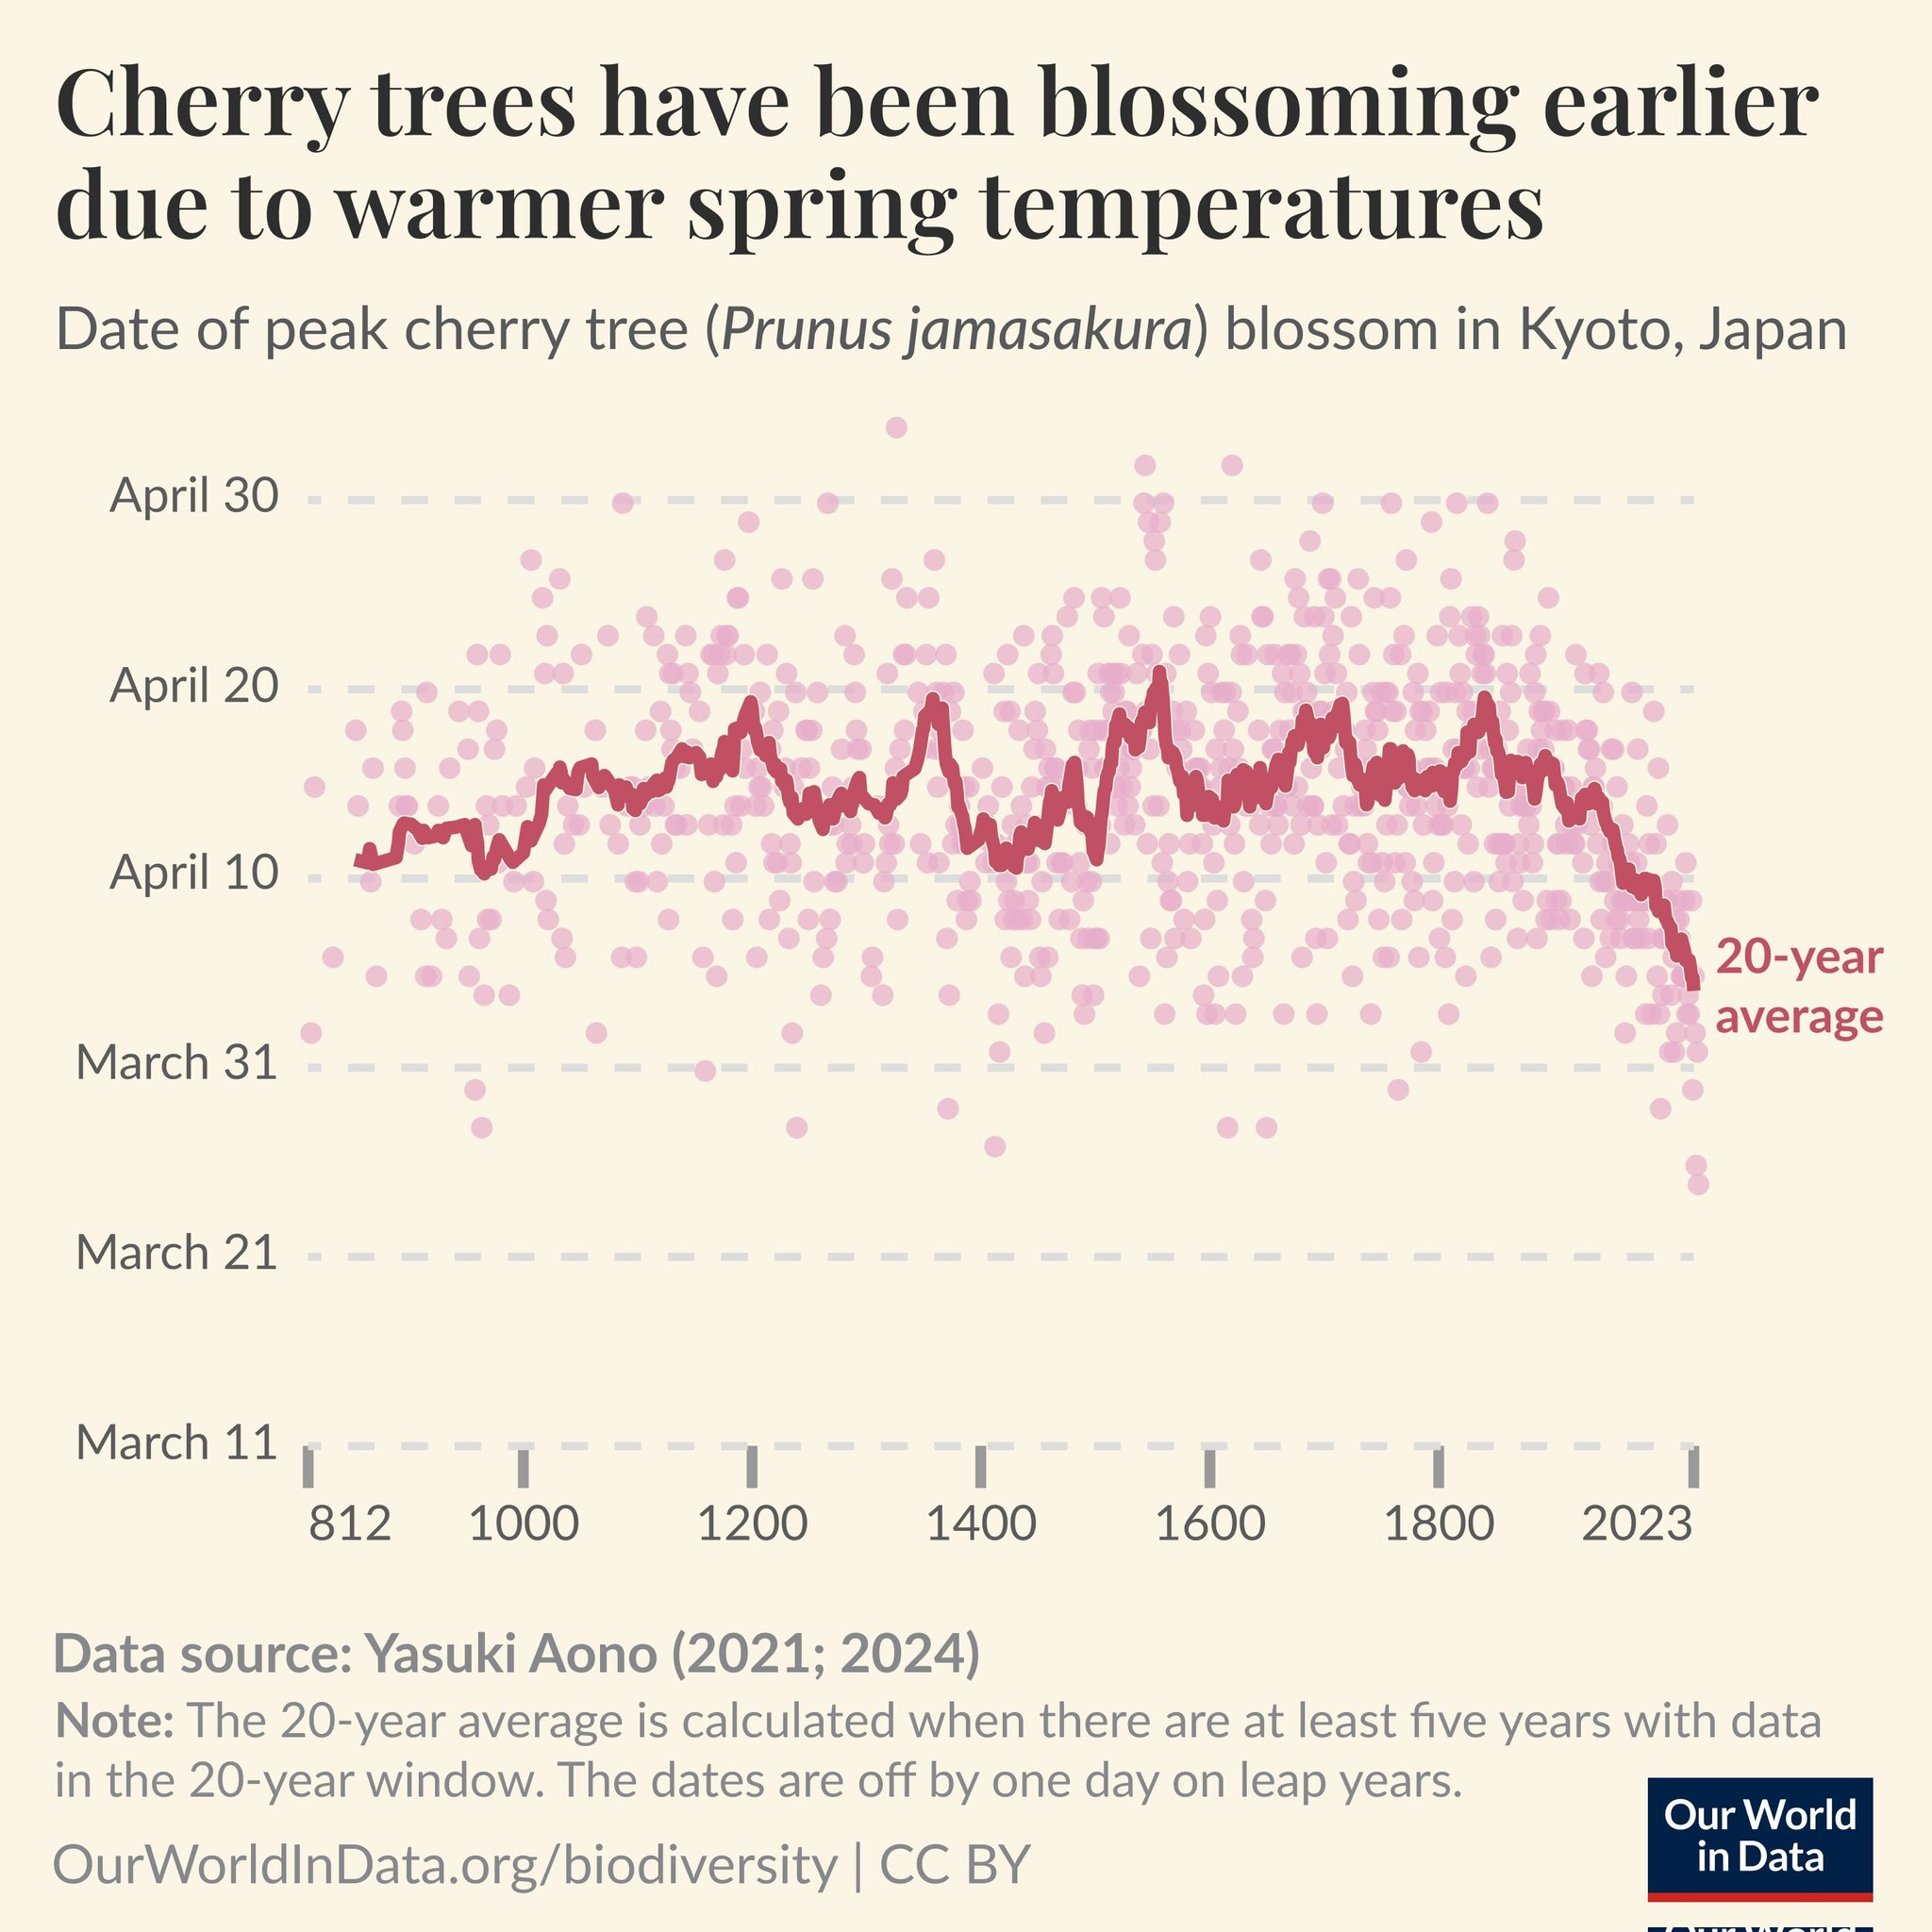
\includegraphics[height=.7\textheight]{cherry_blossoms.JPG}}
\only<8>{\centering\large Proximity and Distance\\~\\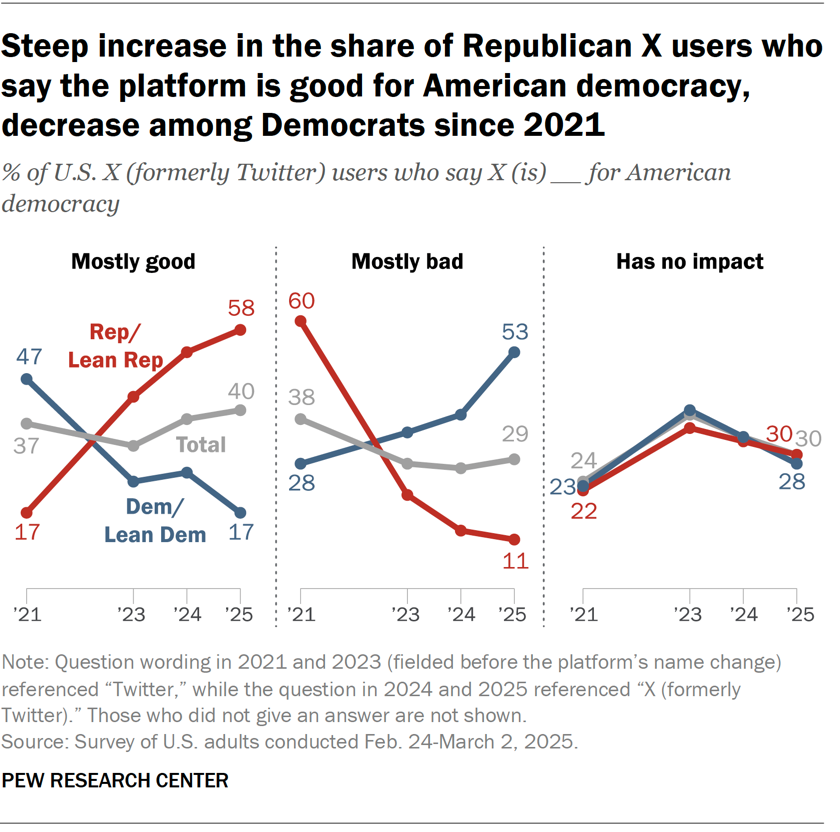
\includegraphics[height=.7\textheight]{views_of_x_partisan_reasoning.png}}
\only<9>{\centering\large Proximity and Distance\\~\\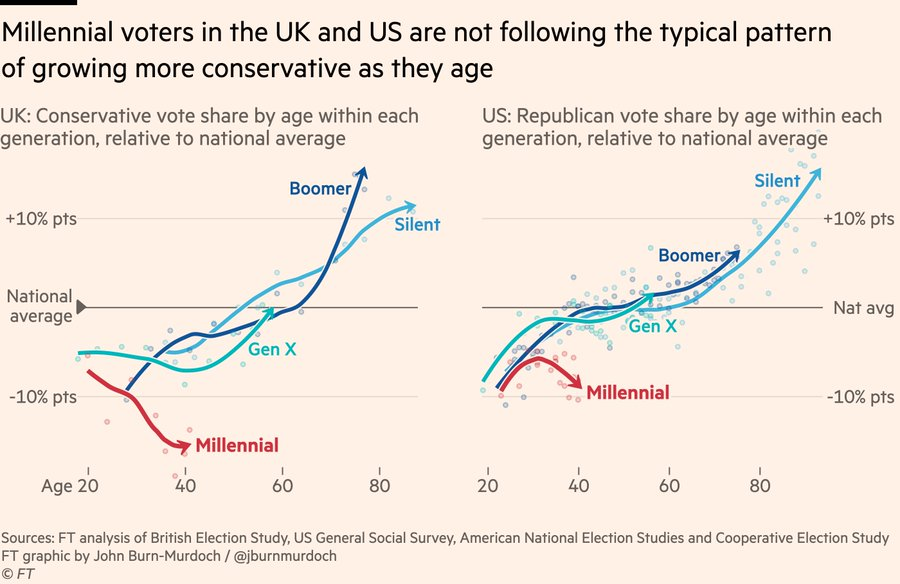
\includegraphics[height=.7\textheight]{ft_partisanship.PNG}}
\only<10>{\centering\large Similarity and Difference\\~\\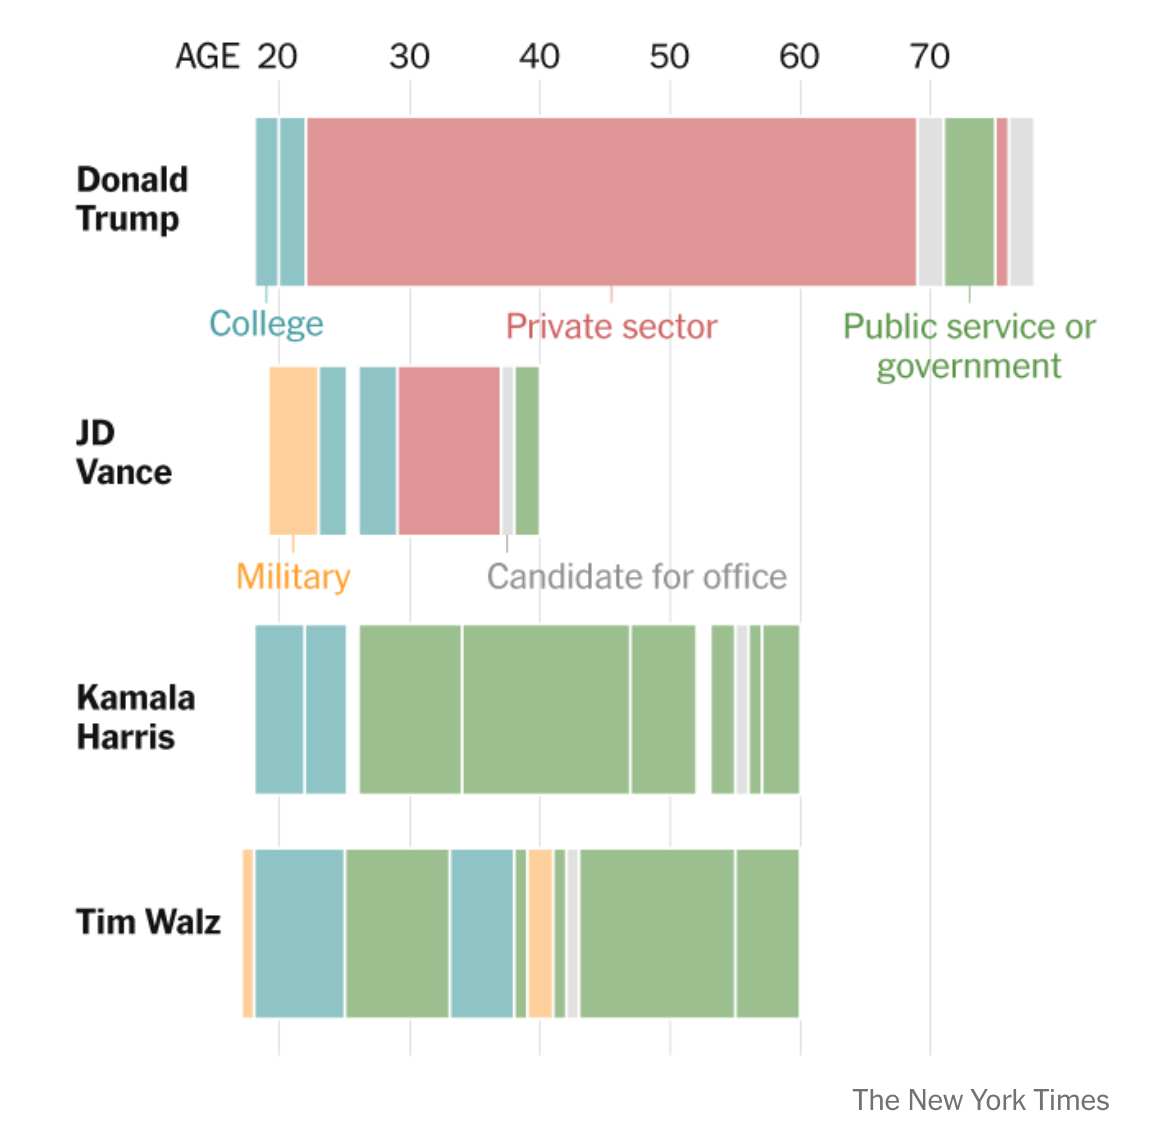
\includegraphics[height=.7\textheight]{nyt_candidate_histories.jpg}}
\only<11>{\centering\large Connectedness\\~\\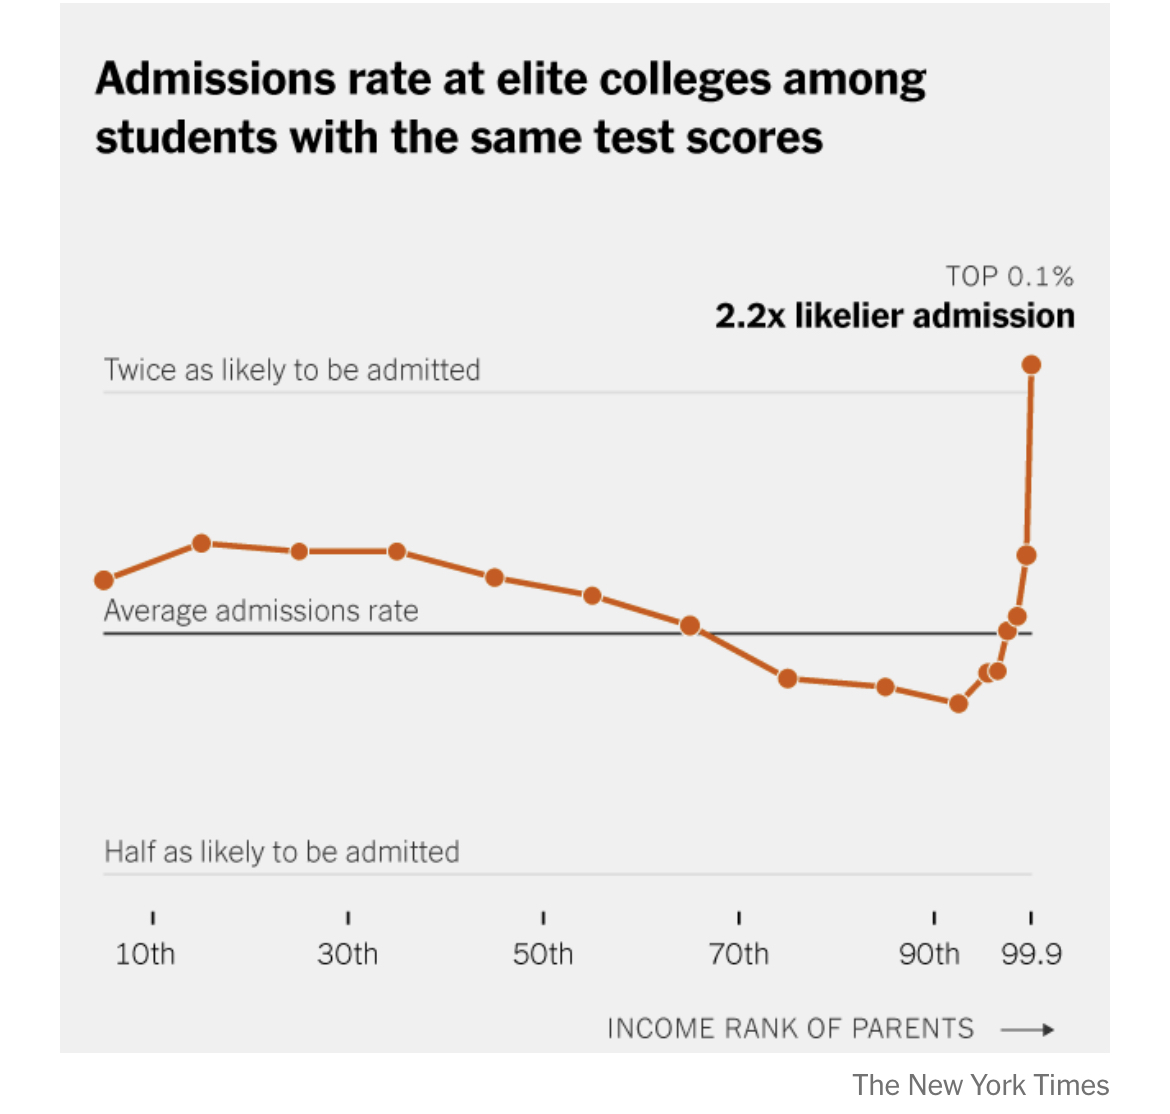
\includegraphics[height=.7\textheight]{nyt_admissions.jpg}}
\only<12>{\centering\large (Dis)Continuity\\~\\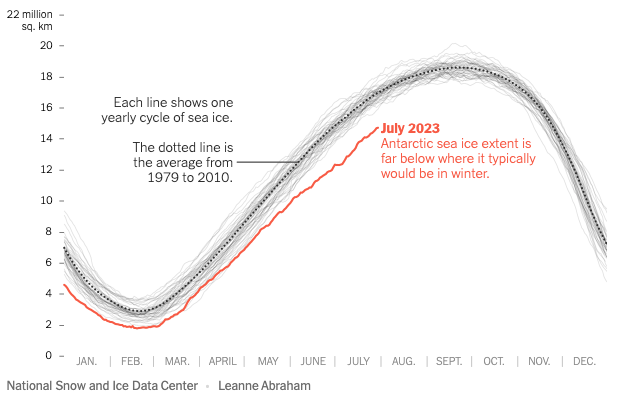
\includegraphics[height=.7\textheight]{nyt_antarctic_ice.png}}
\only<13>{\centering\large (Dis)Continuity\\~\\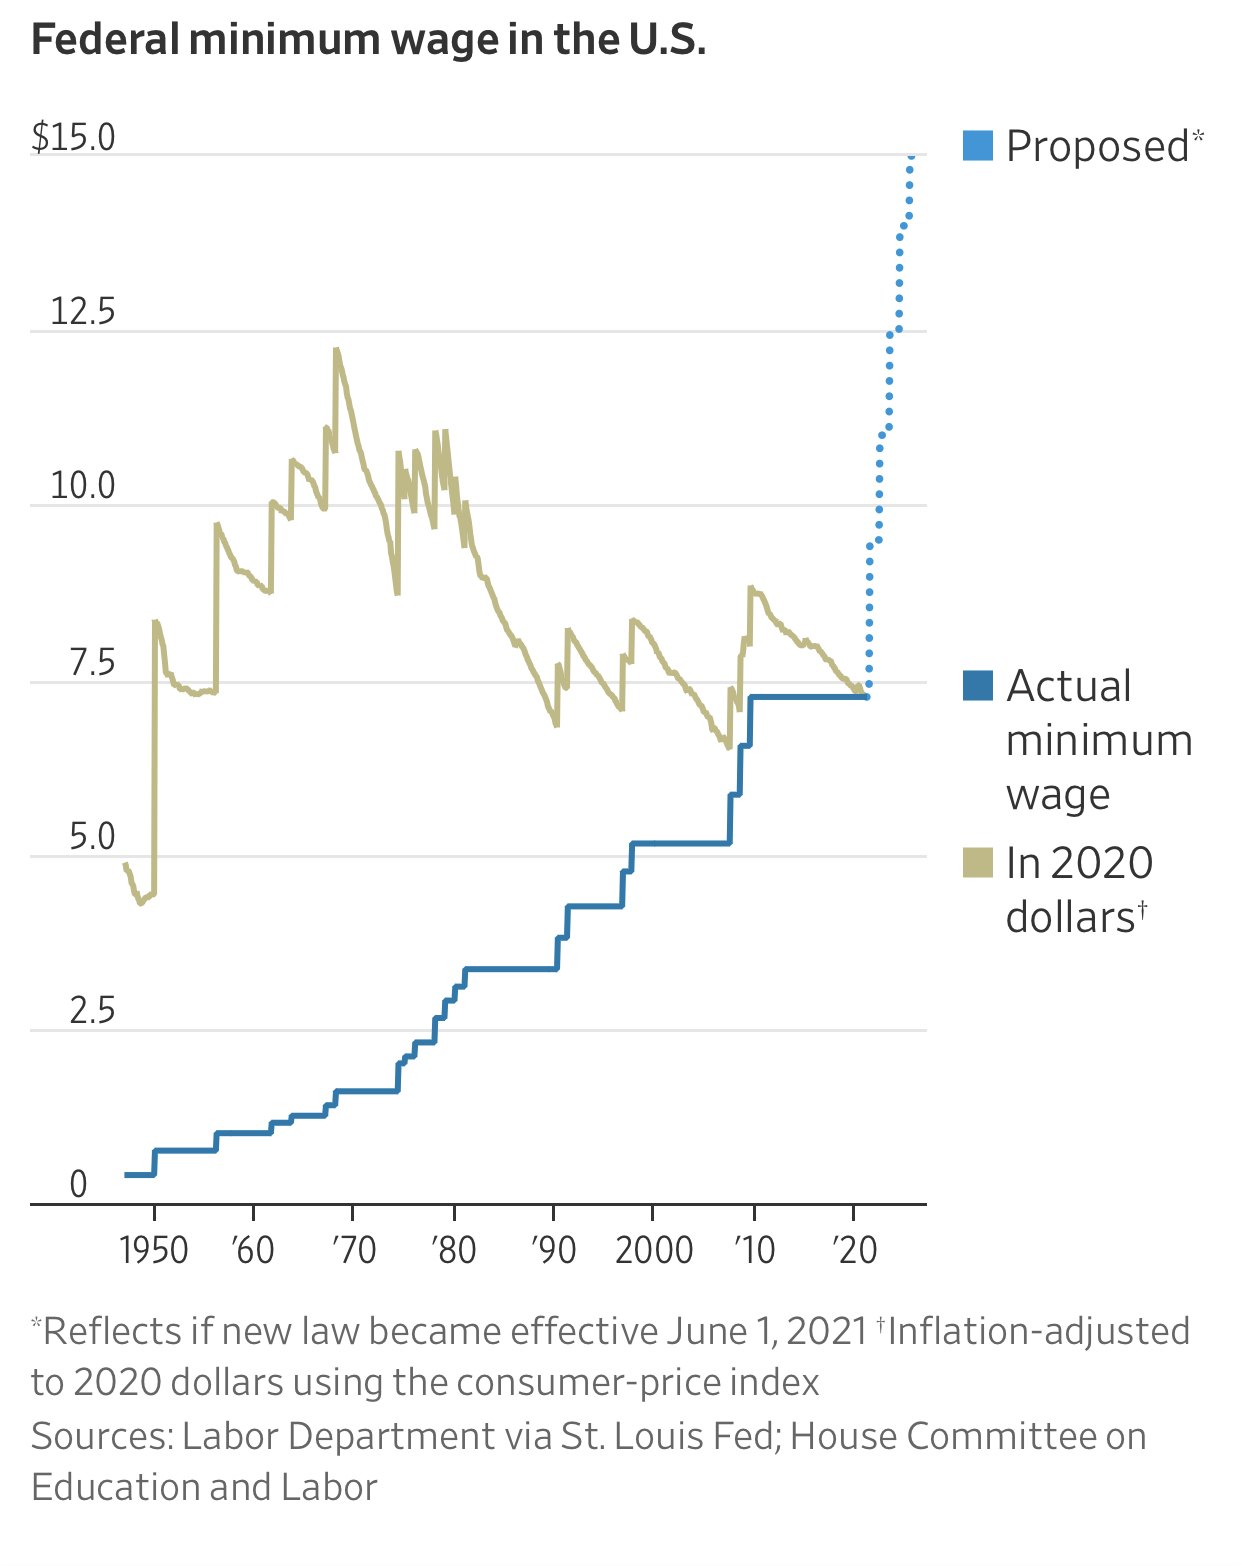
\includegraphics[height=.7\textheight]{wsj_minimum_wage.jpg}}
\only<14>{\centering\large Closure\\~\\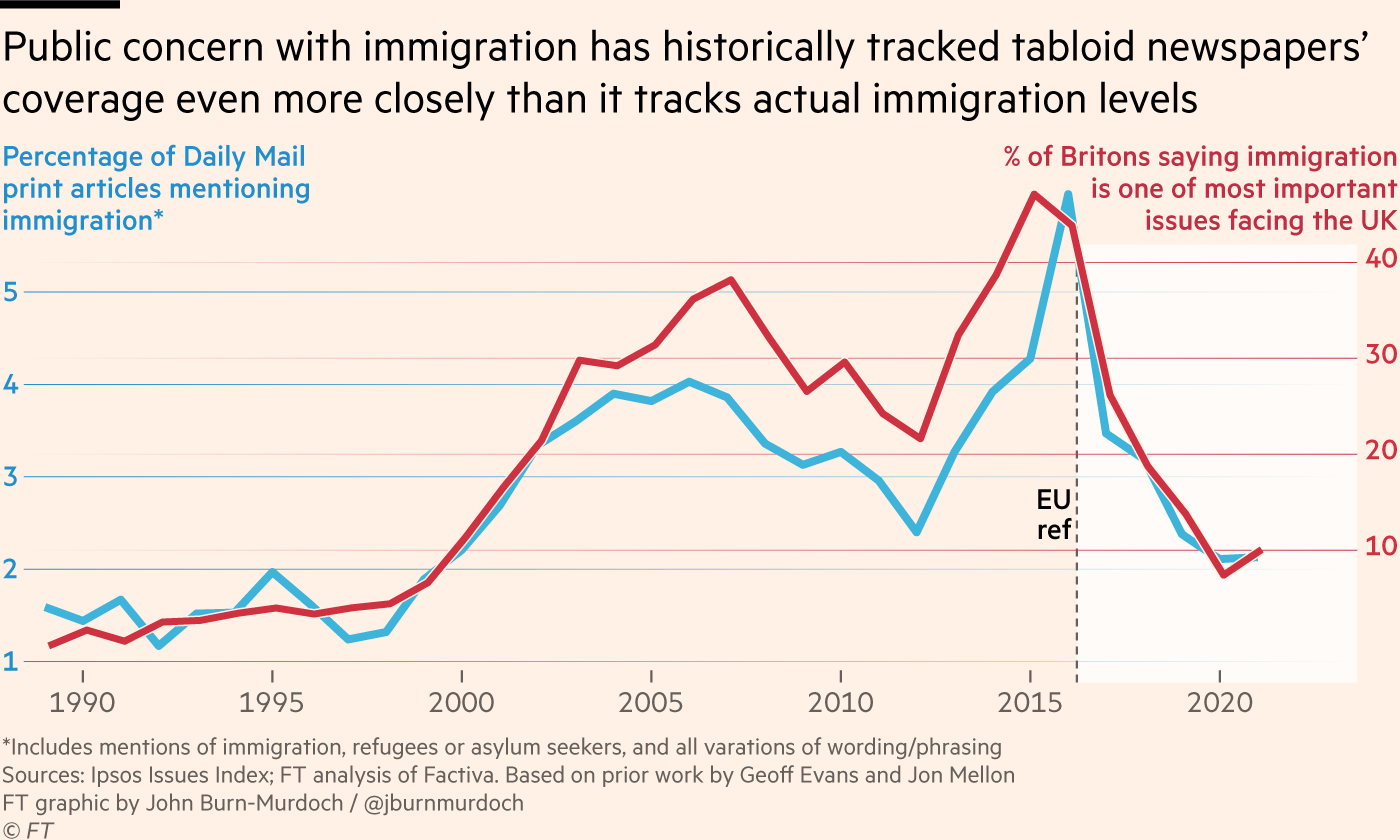
\includegraphics[height=.7\textheight]{ft_immigration.png}}
\only<15>{\centering\large Closure\\~\\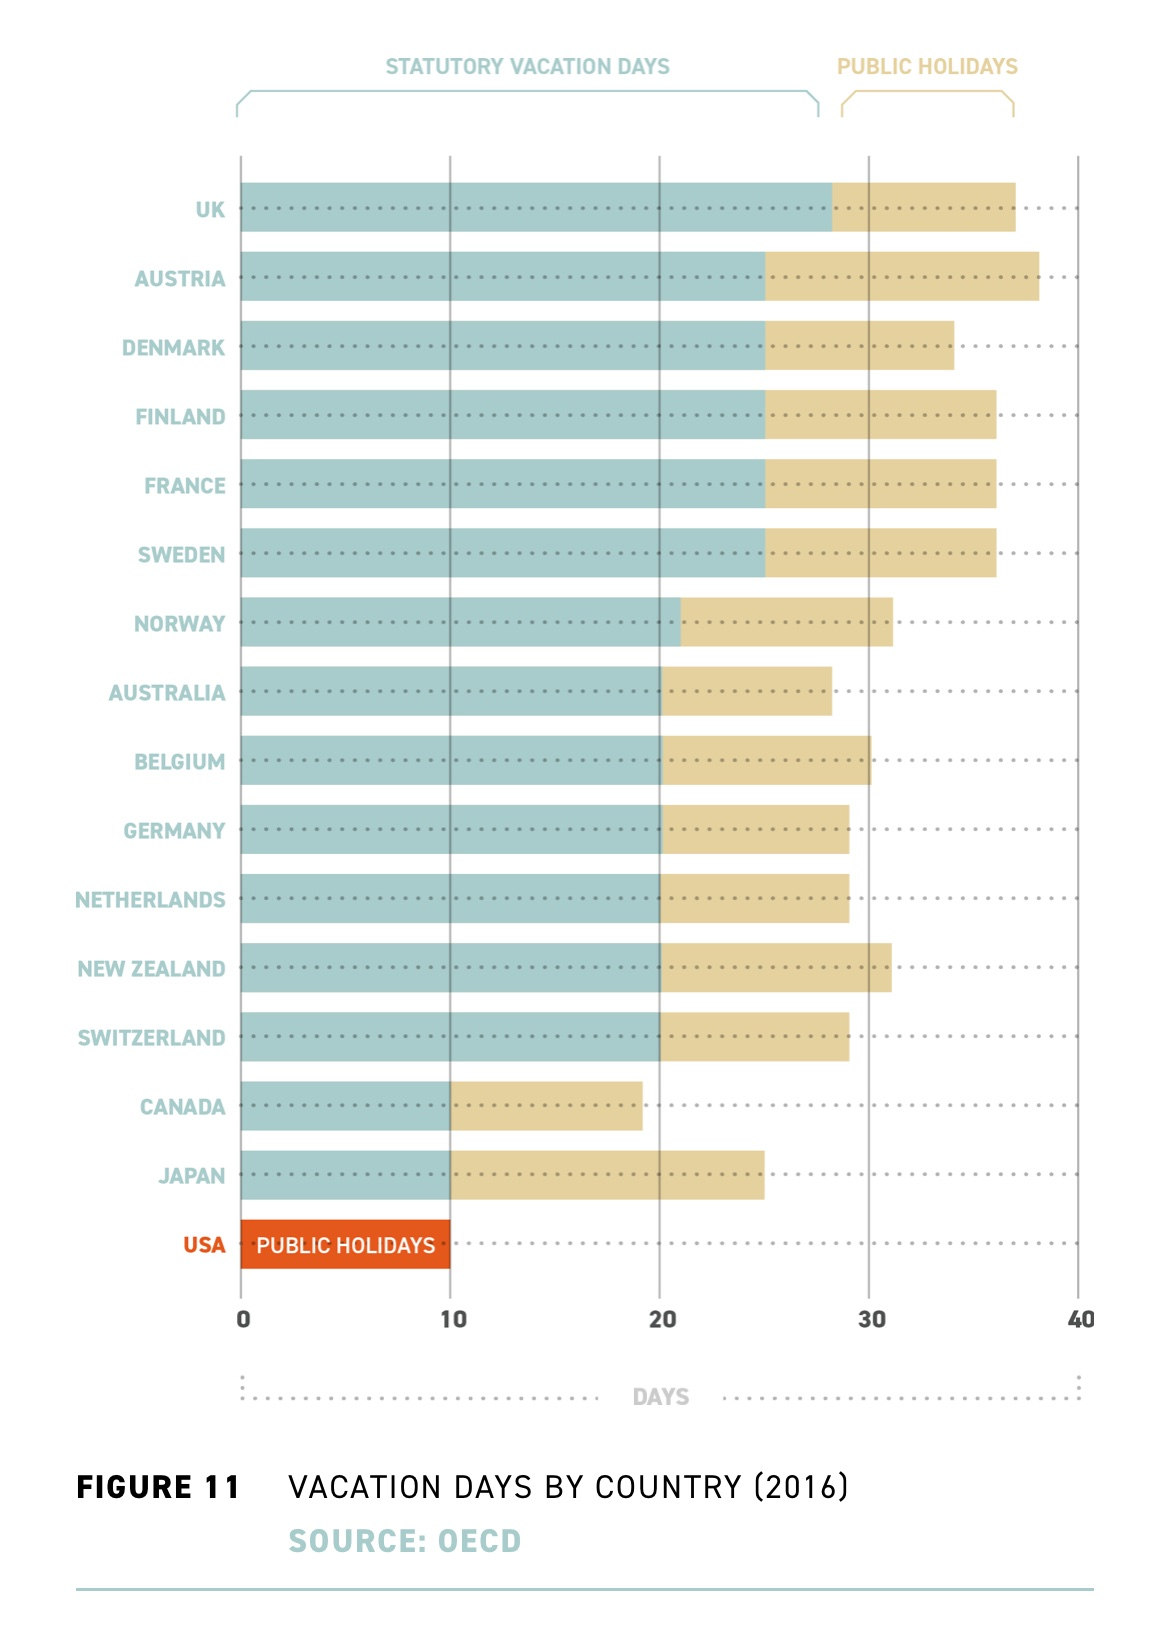
\includegraphics[height=.7\textheight]{vacation_days.jpeg}\\\scriptsize Source: People's Policy Project}
\only<16>{\centering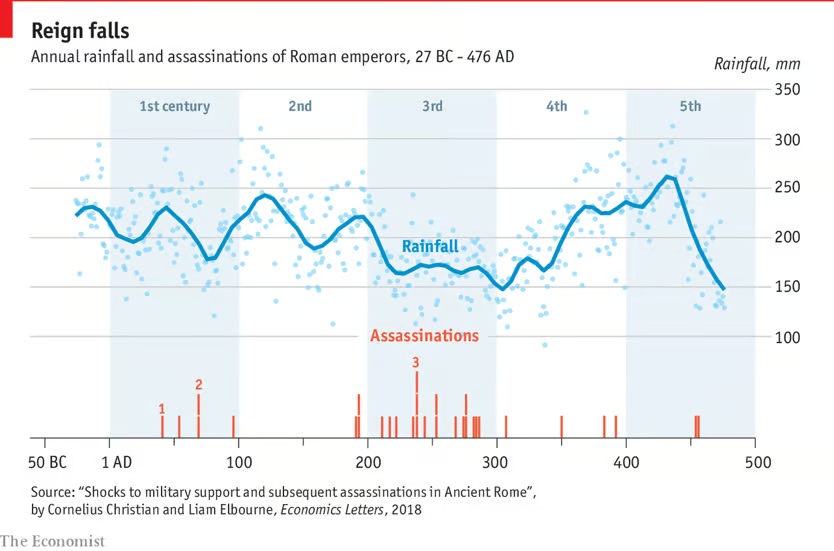
\includegraphics[width=.9\textwidth]{economist_assasinations.png}}
}

%%%%%%%%%%%%%%%%%%%%%%%%%%%%%%%%%%%%%%%%%%%%%%%%%%%%%%%%%%%%%%%%%%
\frame{\frametitle{Parts of a Graph}
    \centering
    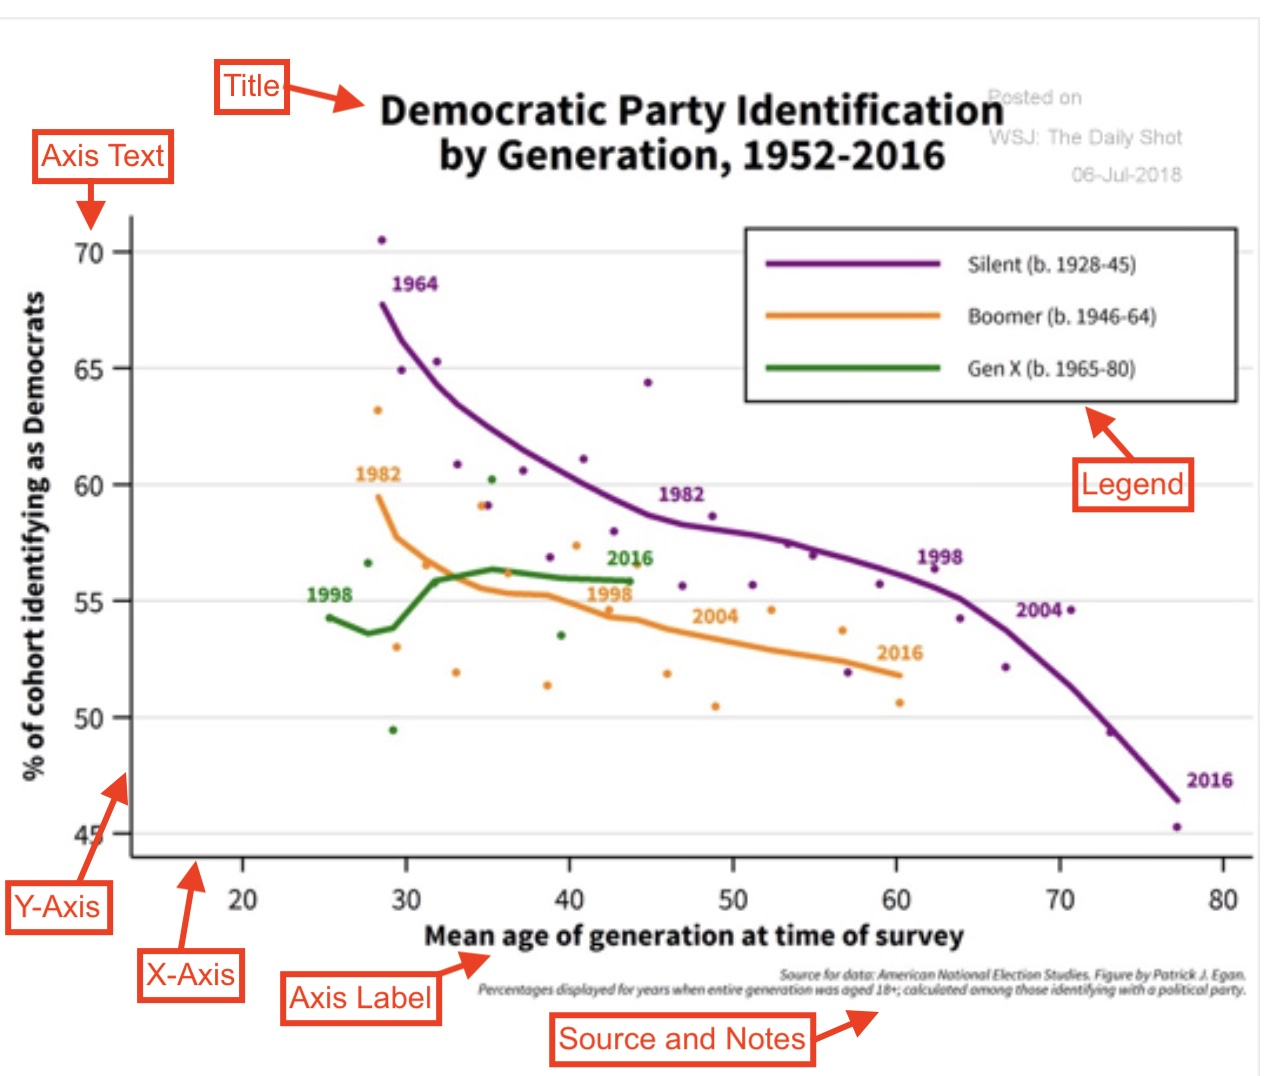
\includegraphics[width=.75\textwidth]{partsofgraph.jpg}
}

%%%%%%%%%%%%%%%%%%%%%%%%%%%%%%%%%%%%%%%%%%%%%%%%%%%%%%%%%%%%%%%%%%
\frame{\frametitle{Designing for Statistics}
\begin{columns}
\column{0.4\textwidth}
\begin{enumerate}[<+->]
        \item<1-> Show the context of the data
        \item<3-> The main axis should show the scale of the data
        \item<5-> Use conventional ordering and meanings
        \item<9-> Data visualizations are paragraphs about data
        \item<11-> Limit cognitive load
        \item<13-> No pie charts
        \item<14-> Not all data should be in a chart
    \end{enumerate}
\column{0.6\textwidth}
\centering
\only<1>{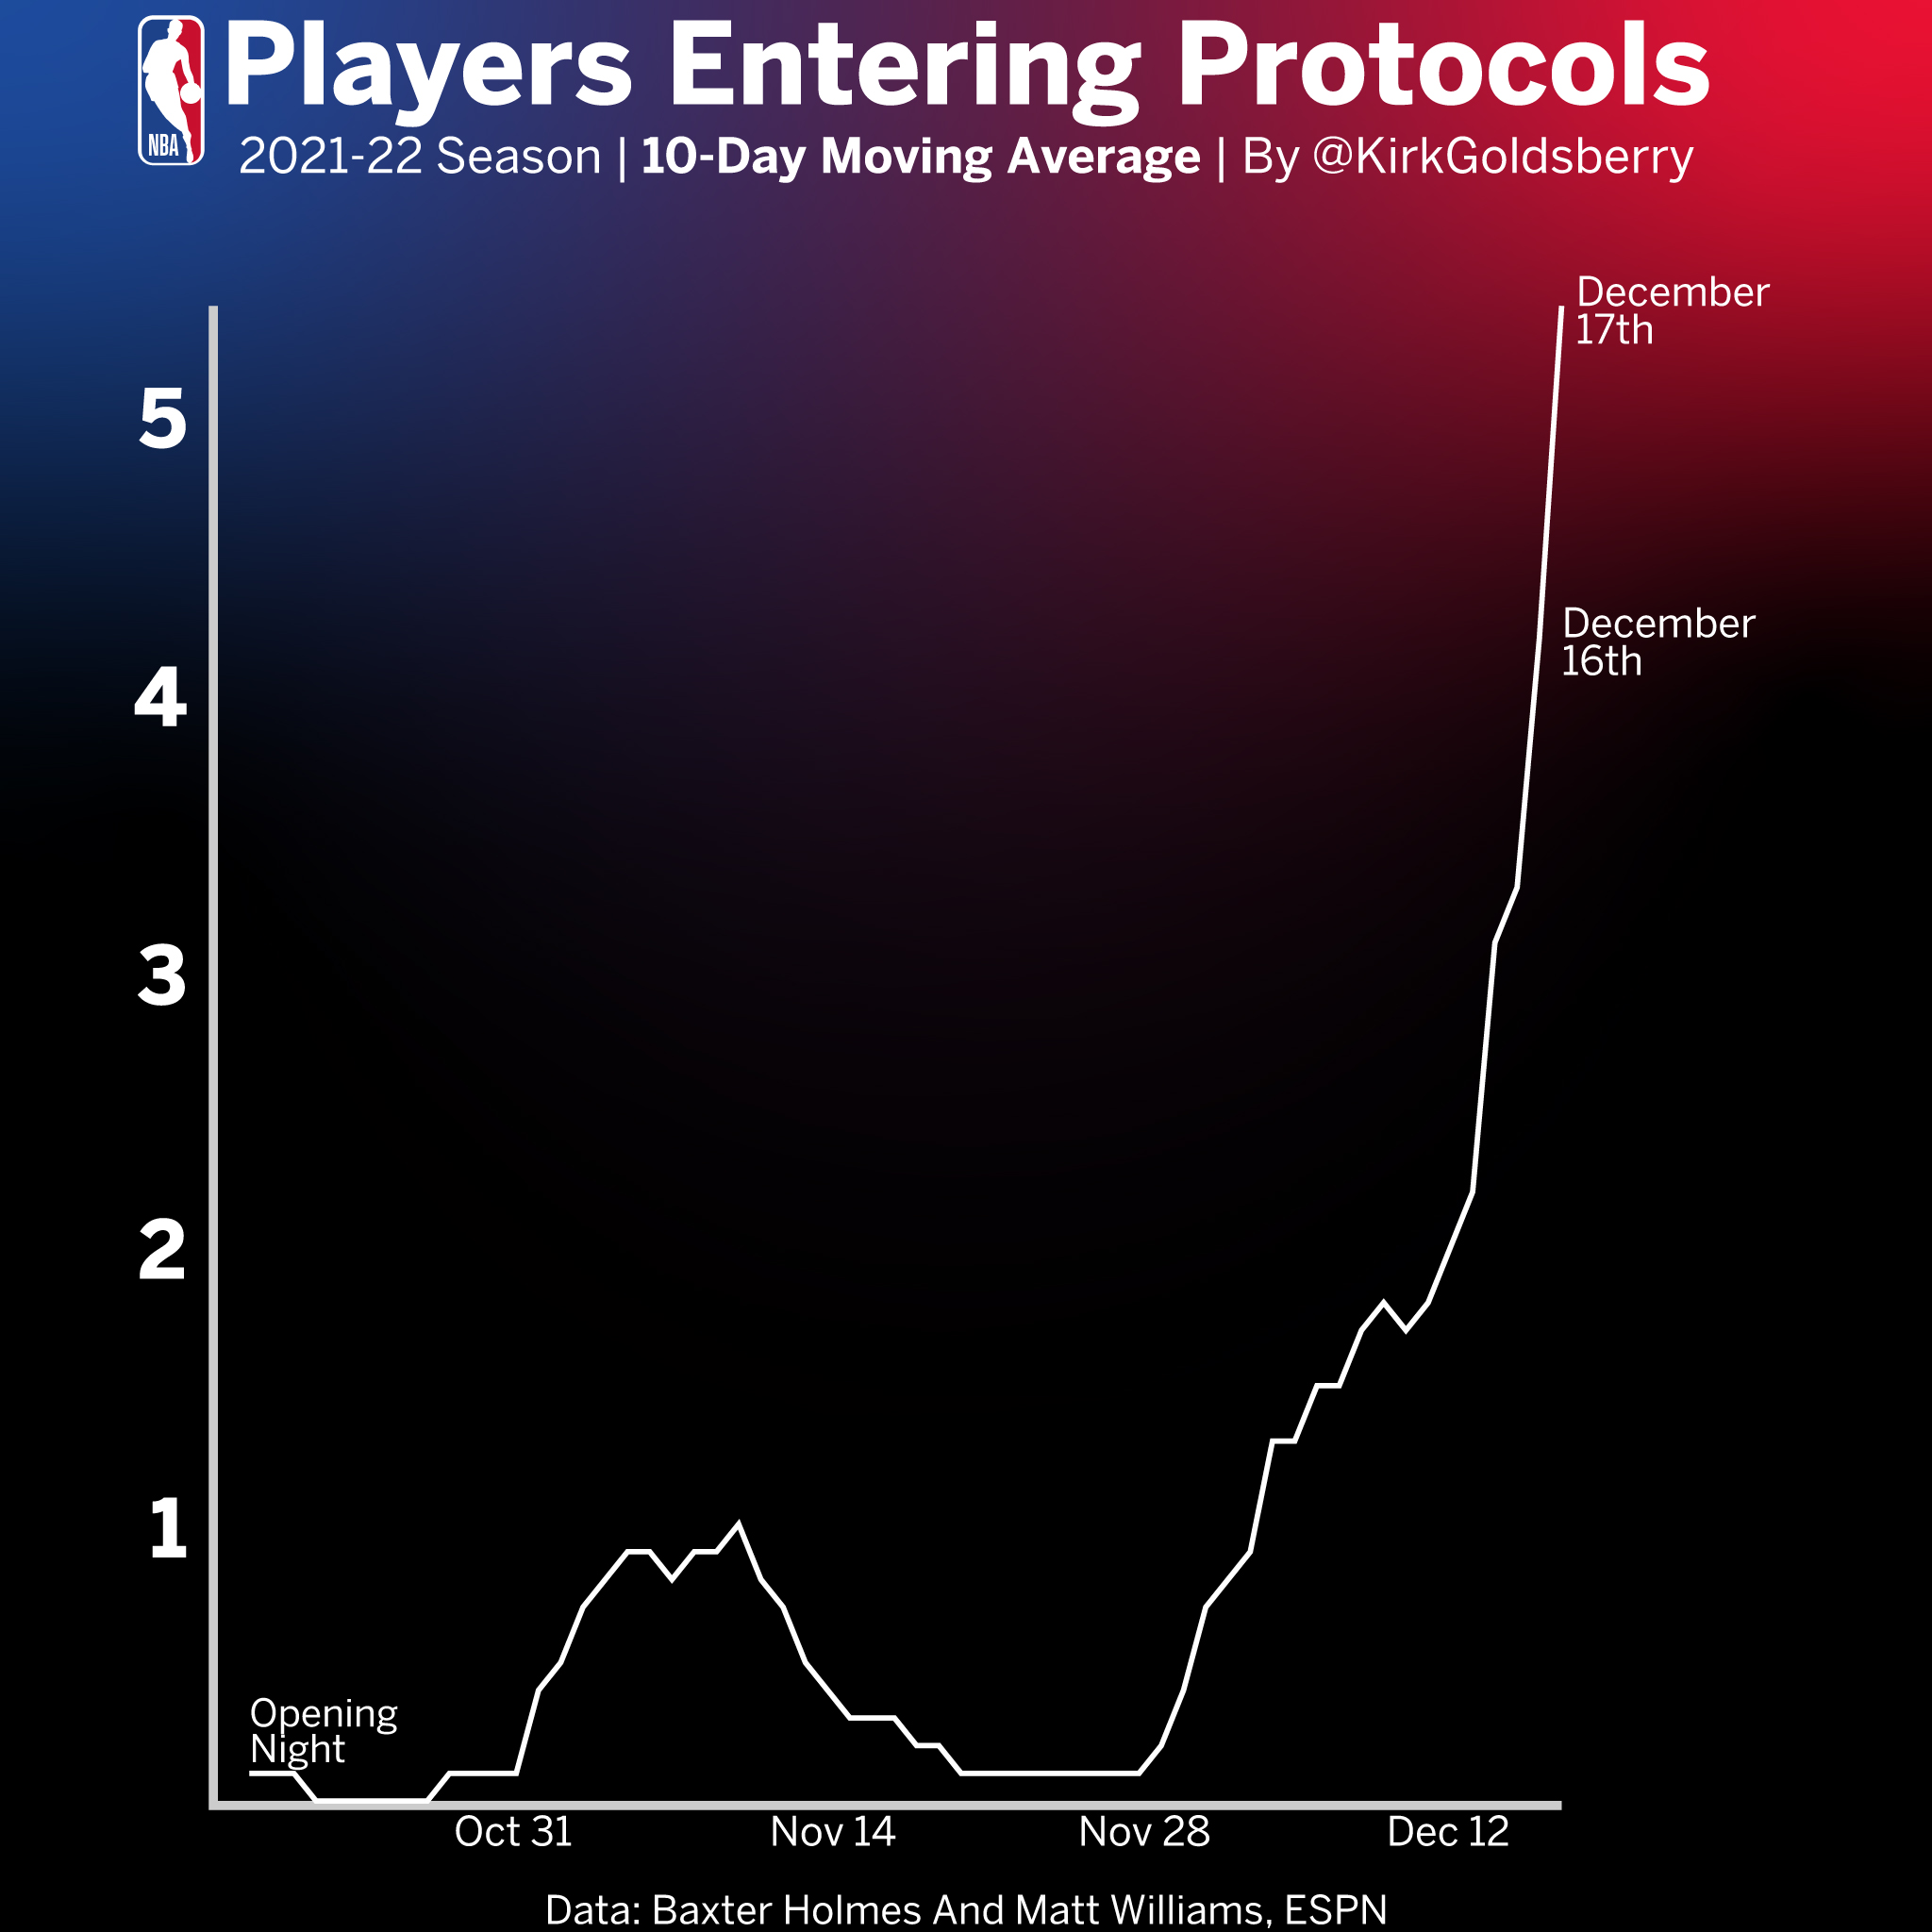
\includegraphics[width=\textwidth]{nba_covid.jpg}}
\only<2>{
    \begin{minipage}{0.48\textwidth}
        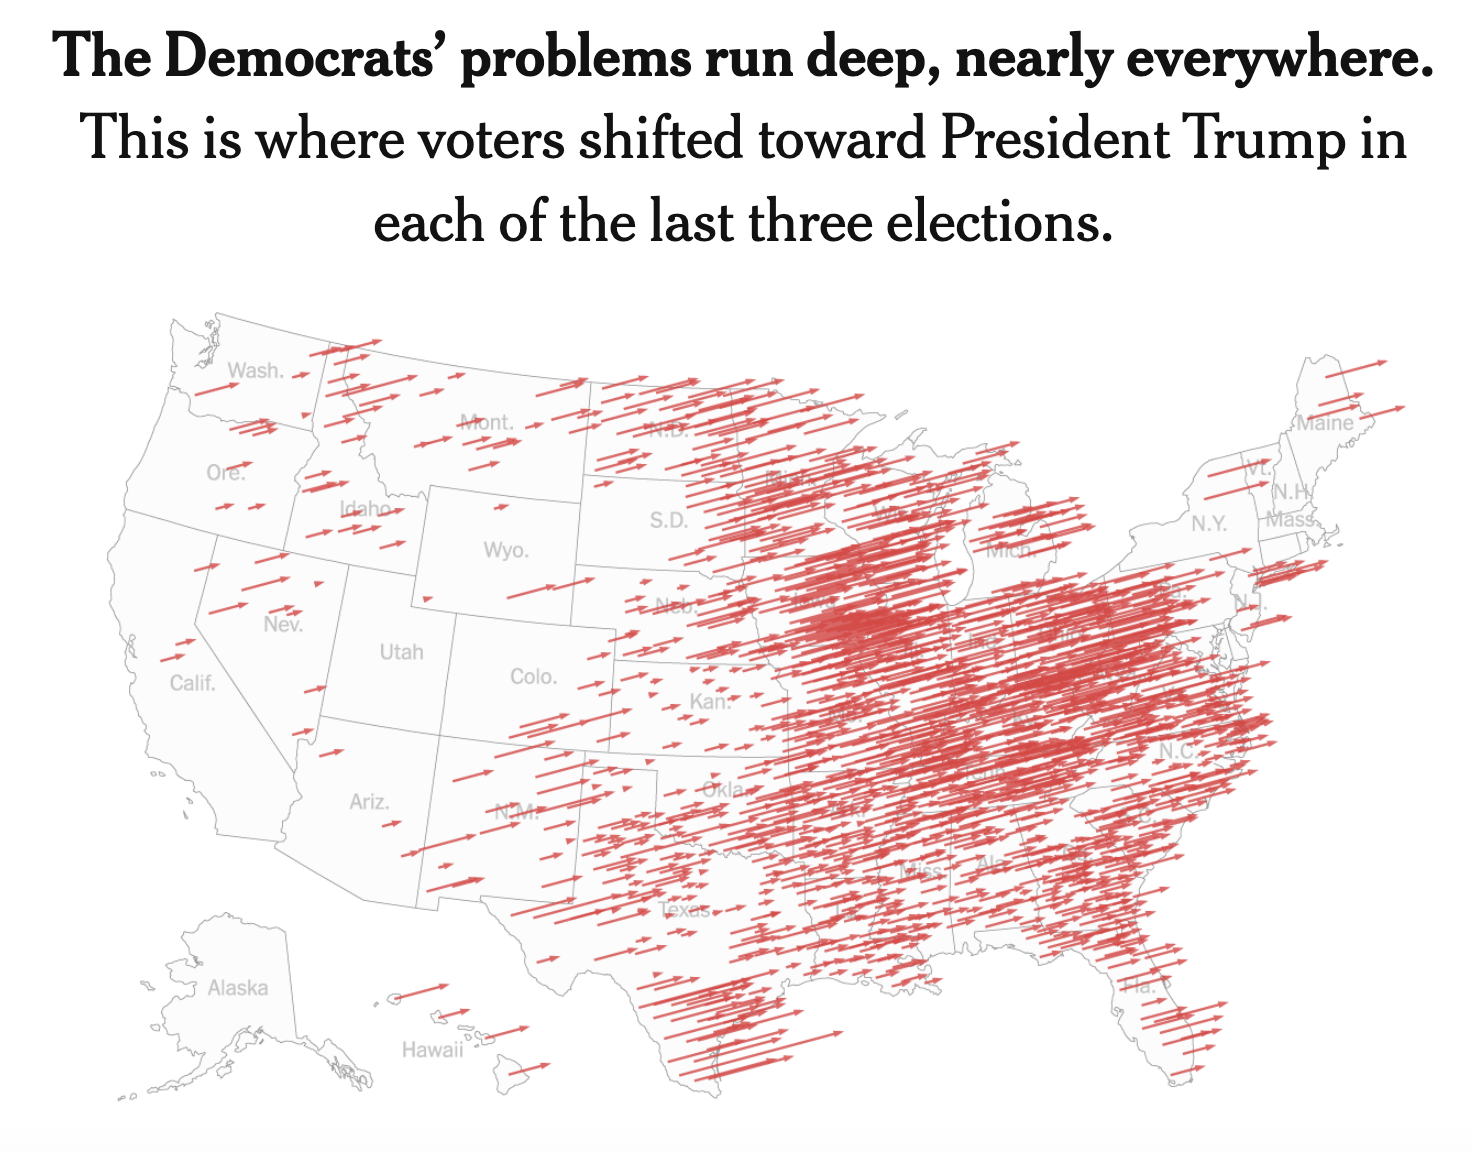
\includegraphics[width=\linewidth]{nyt_county_shift_red.png}
    \end{minipage}
    \hfill
    \begin{minipage}{0.48\textwidth}
        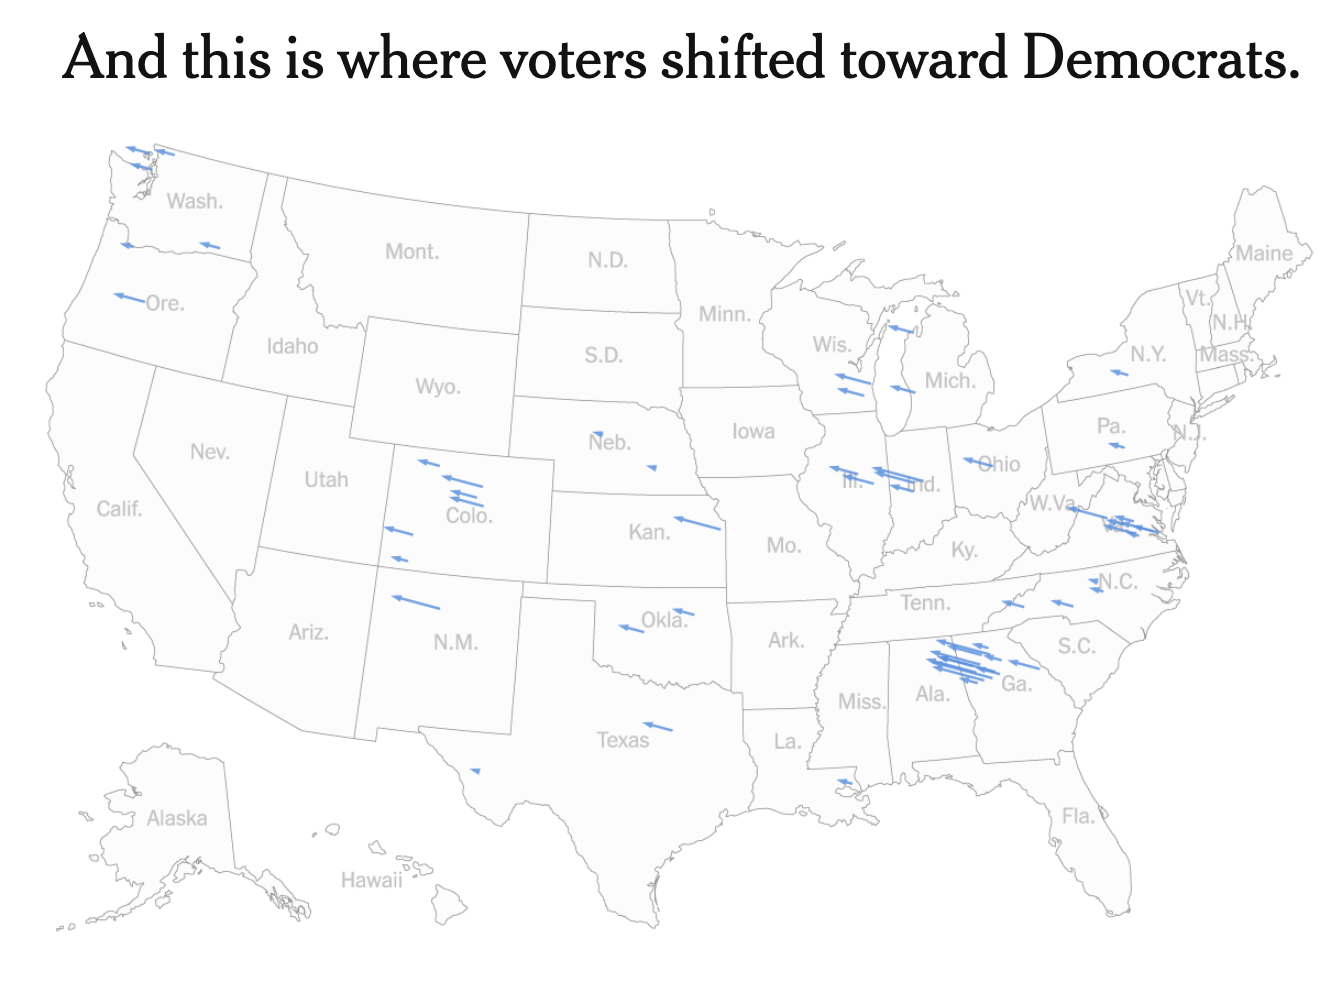
\includegraphics[width=\linewidth]{nyt_county_shift_blue.png}
    \end{minipage}
}
\only<3>{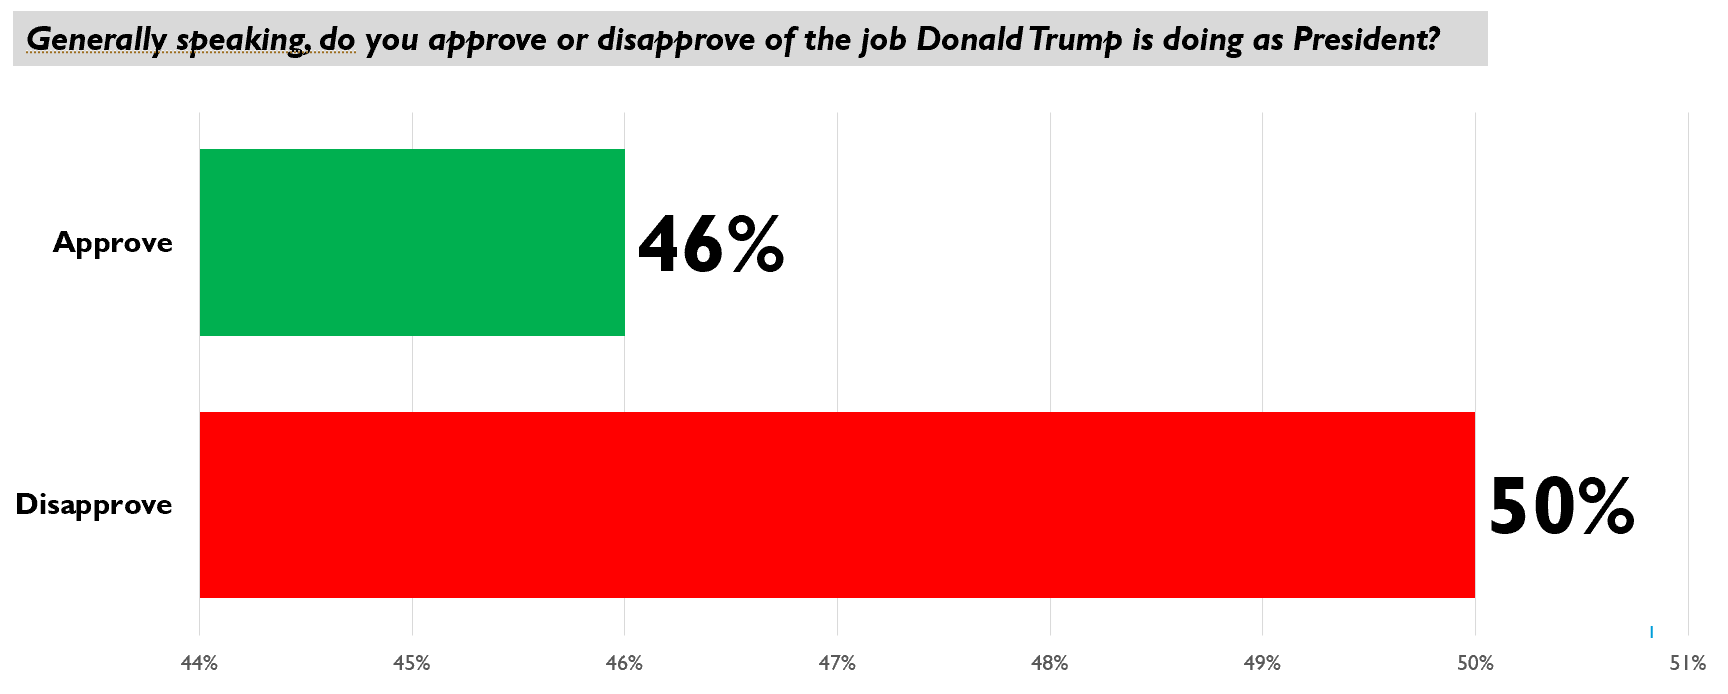
\includegraphics[width=\textwidth]{truncated_axis_spr.png}\\\scriptsize Source: Susquehanna Polling \& Research}
\only<4>{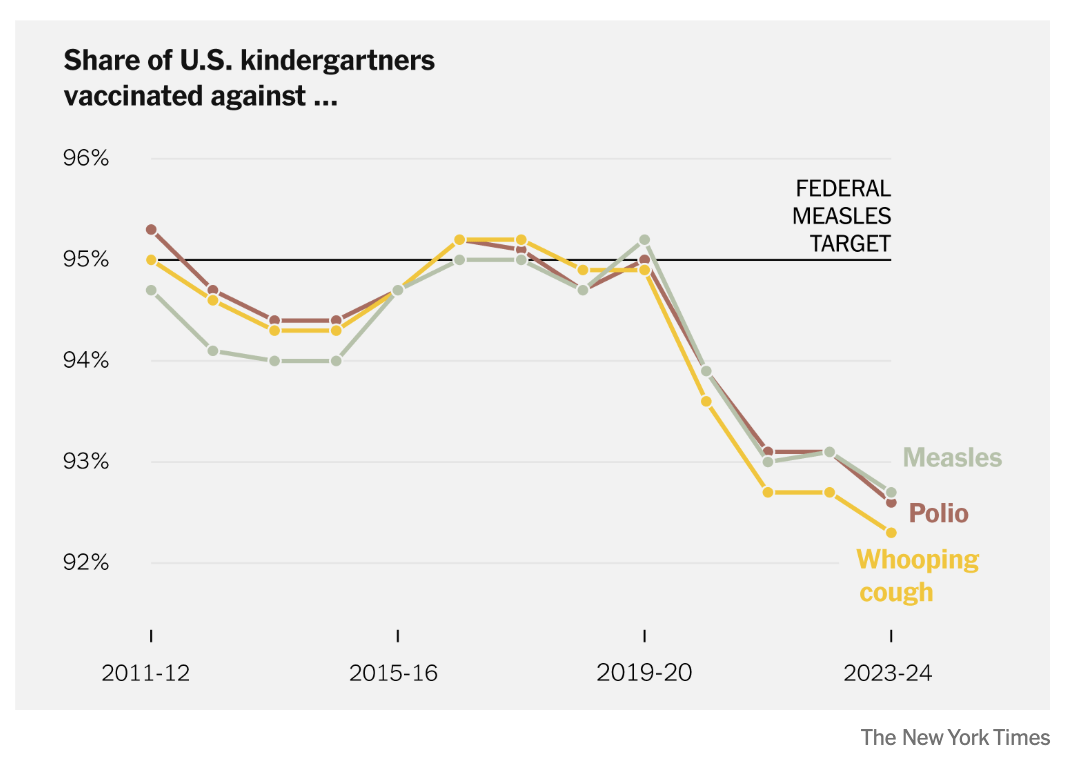
\includegraphics[width=\textwidth]{nyt_vaccination.png}}
\only<5>{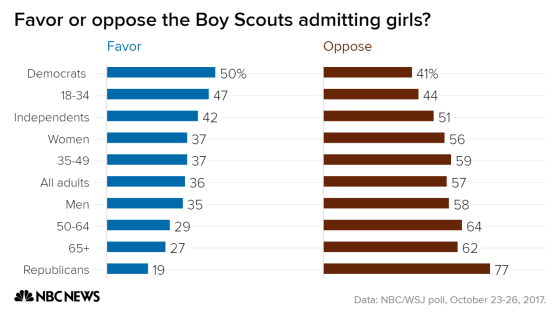
\includegraphics[width=\textwidth]{nbc_boy_scouts.png}}
\only<6>{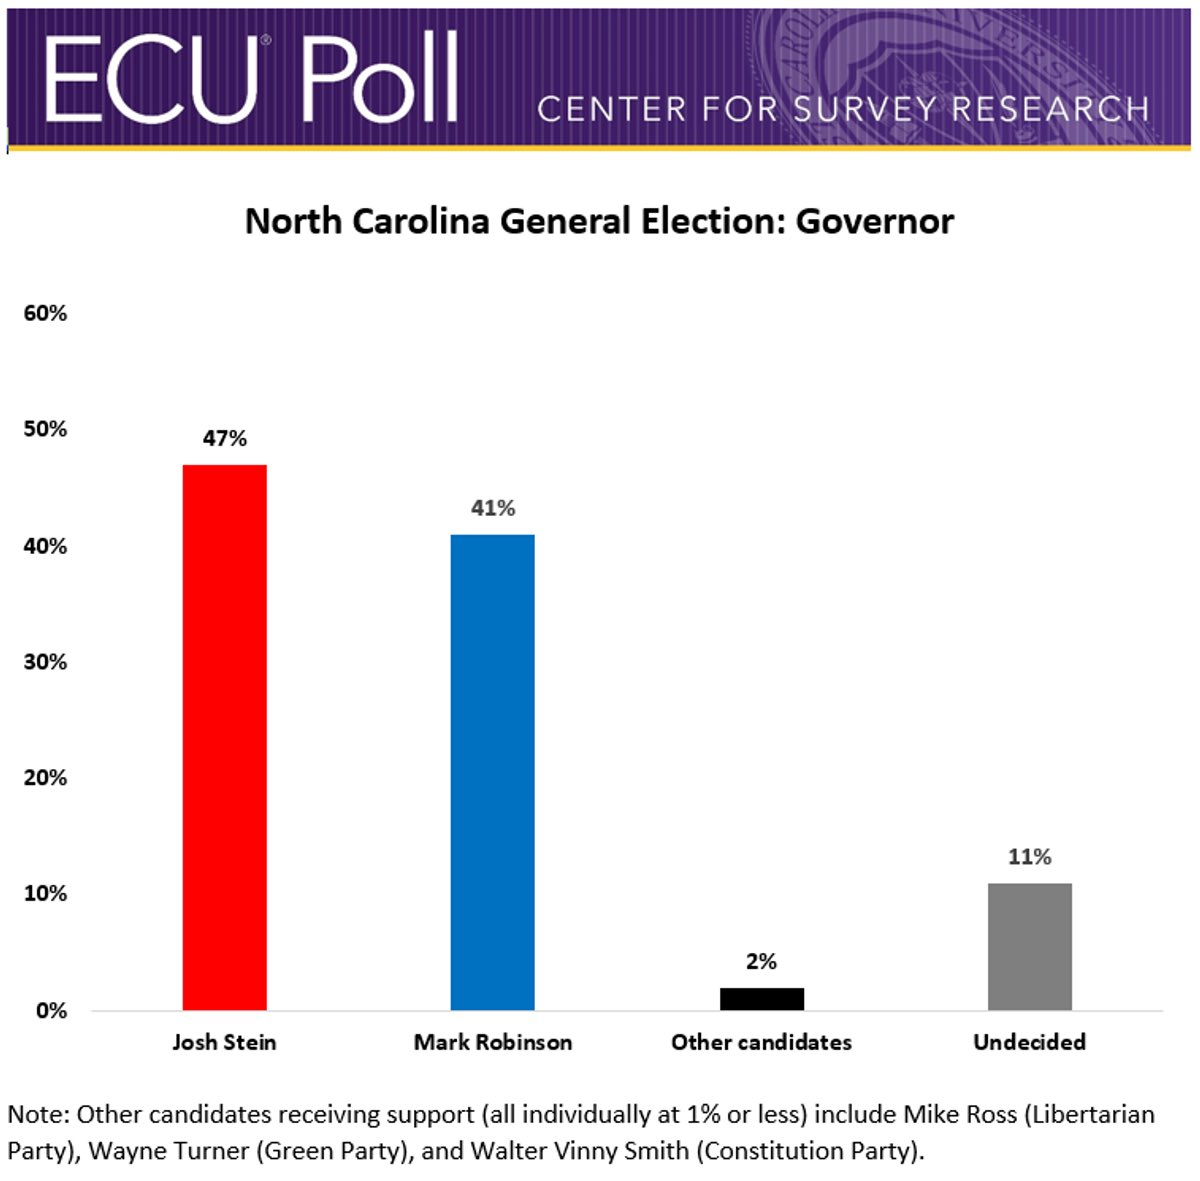
\includegraphics[width=\textwidth]{stein_robinson_poll.jpeg}}
\only<7>{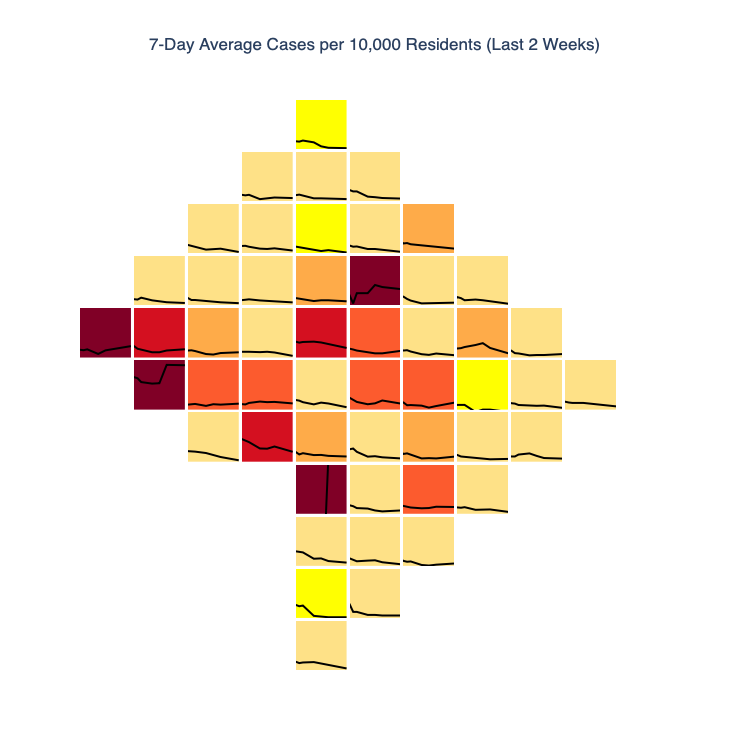
\includegraphics[width=\textwidth]{DC_covid.png}}
\only<8>{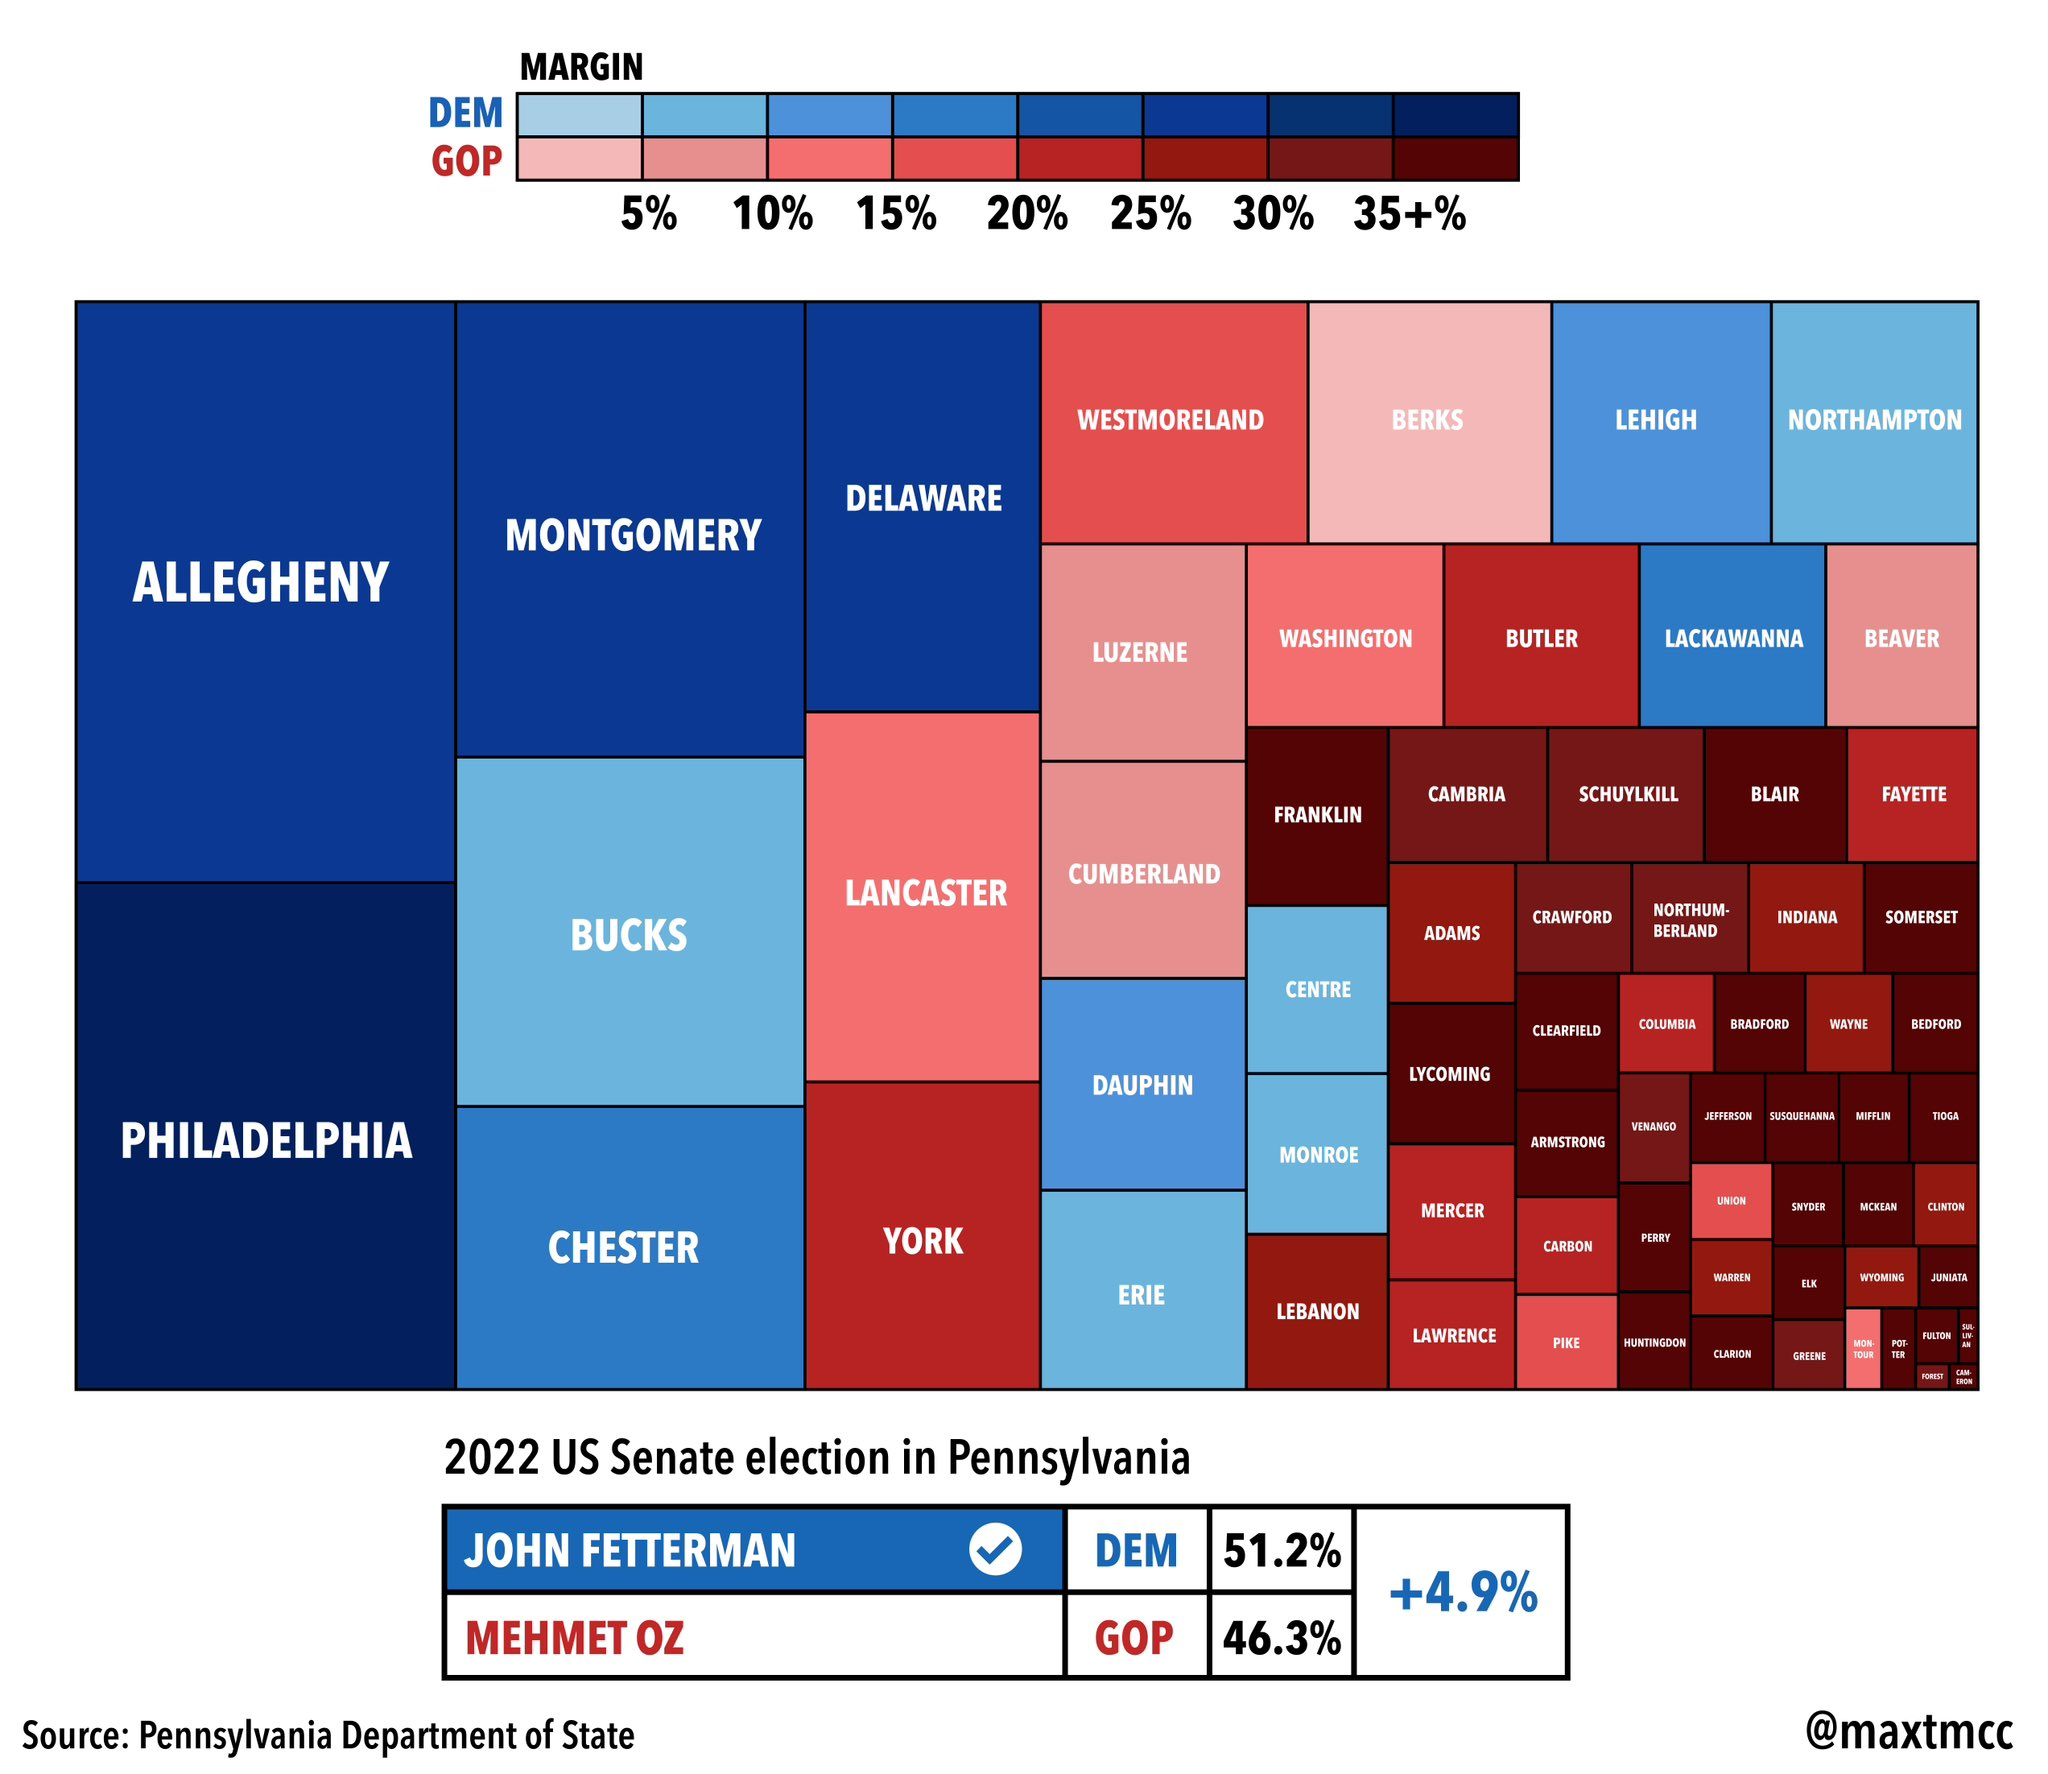
\includegraphics[width=\textwidth]{pa_sen_result.JPG}}
\only<9>{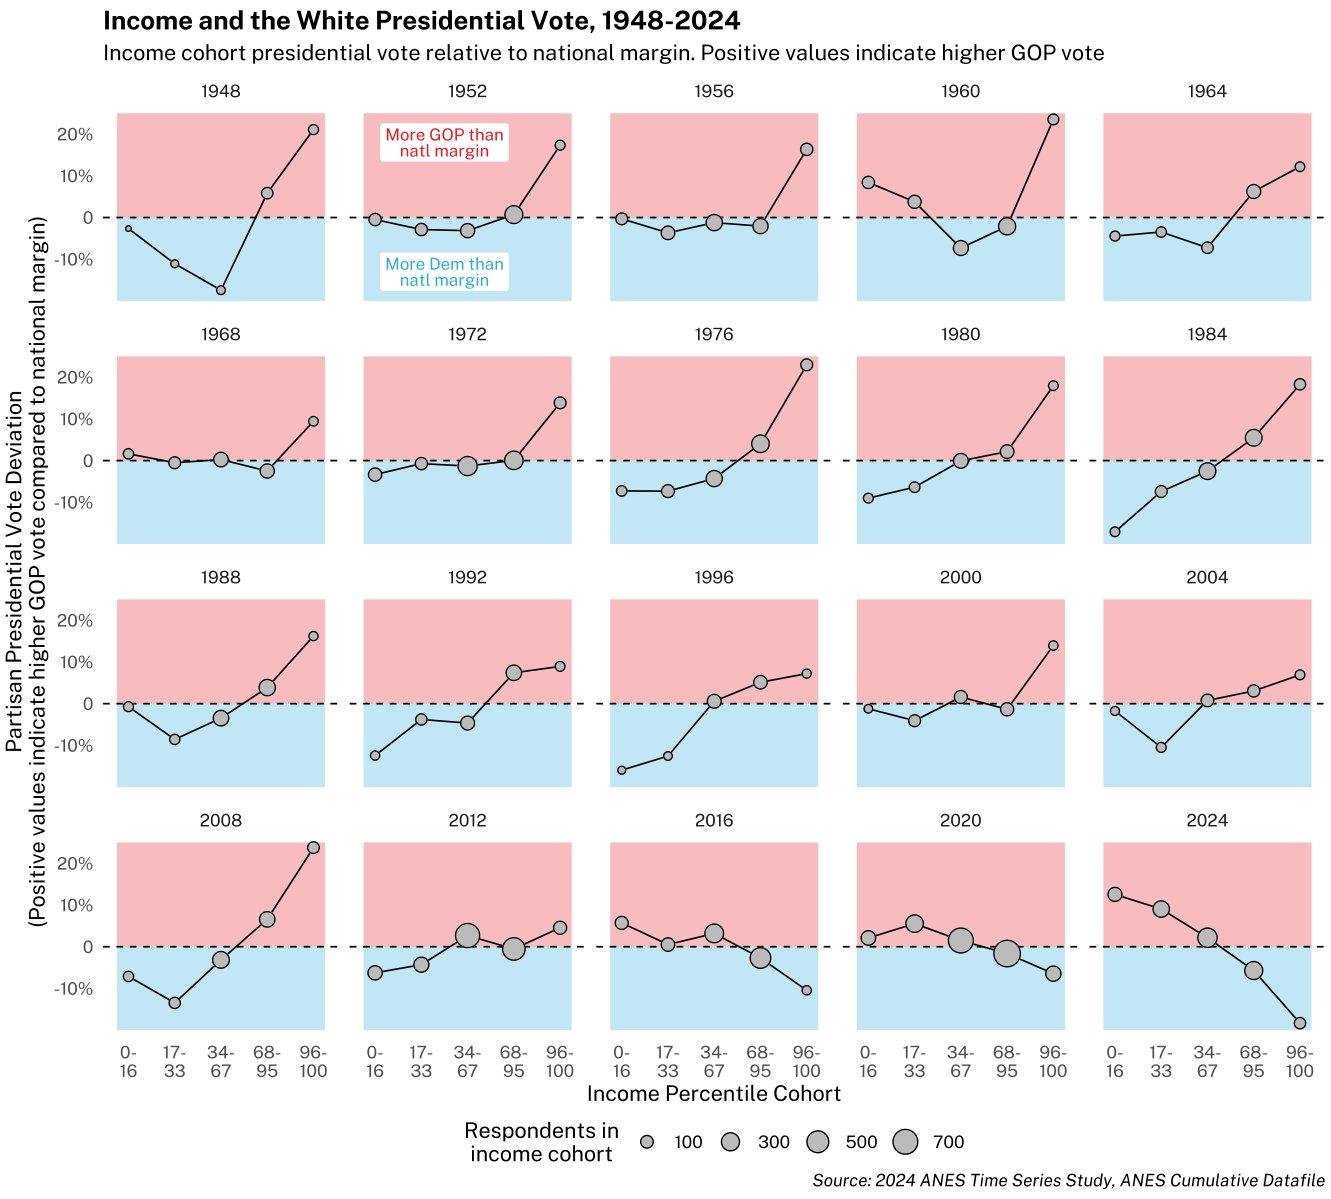
\includegraphics[width=\textwidth]{income_pres_vote.jpeg}\\\scriptsize Source: @thomasjwood}
\only<10>{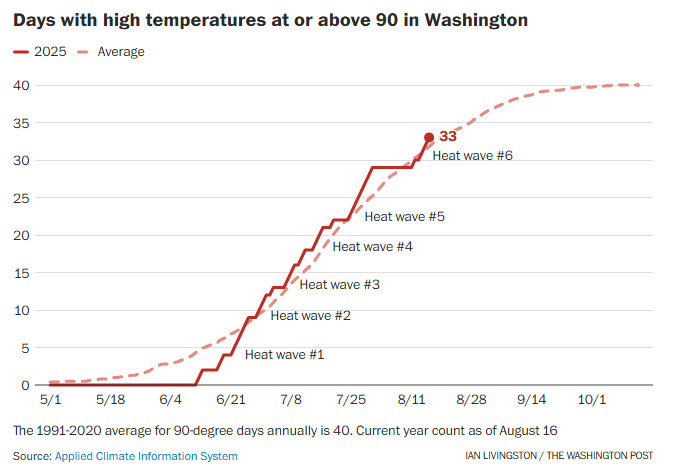
\includegraphics[width=\textwidth]{wapo_2025_90_degree_days.png}}
\only<11>{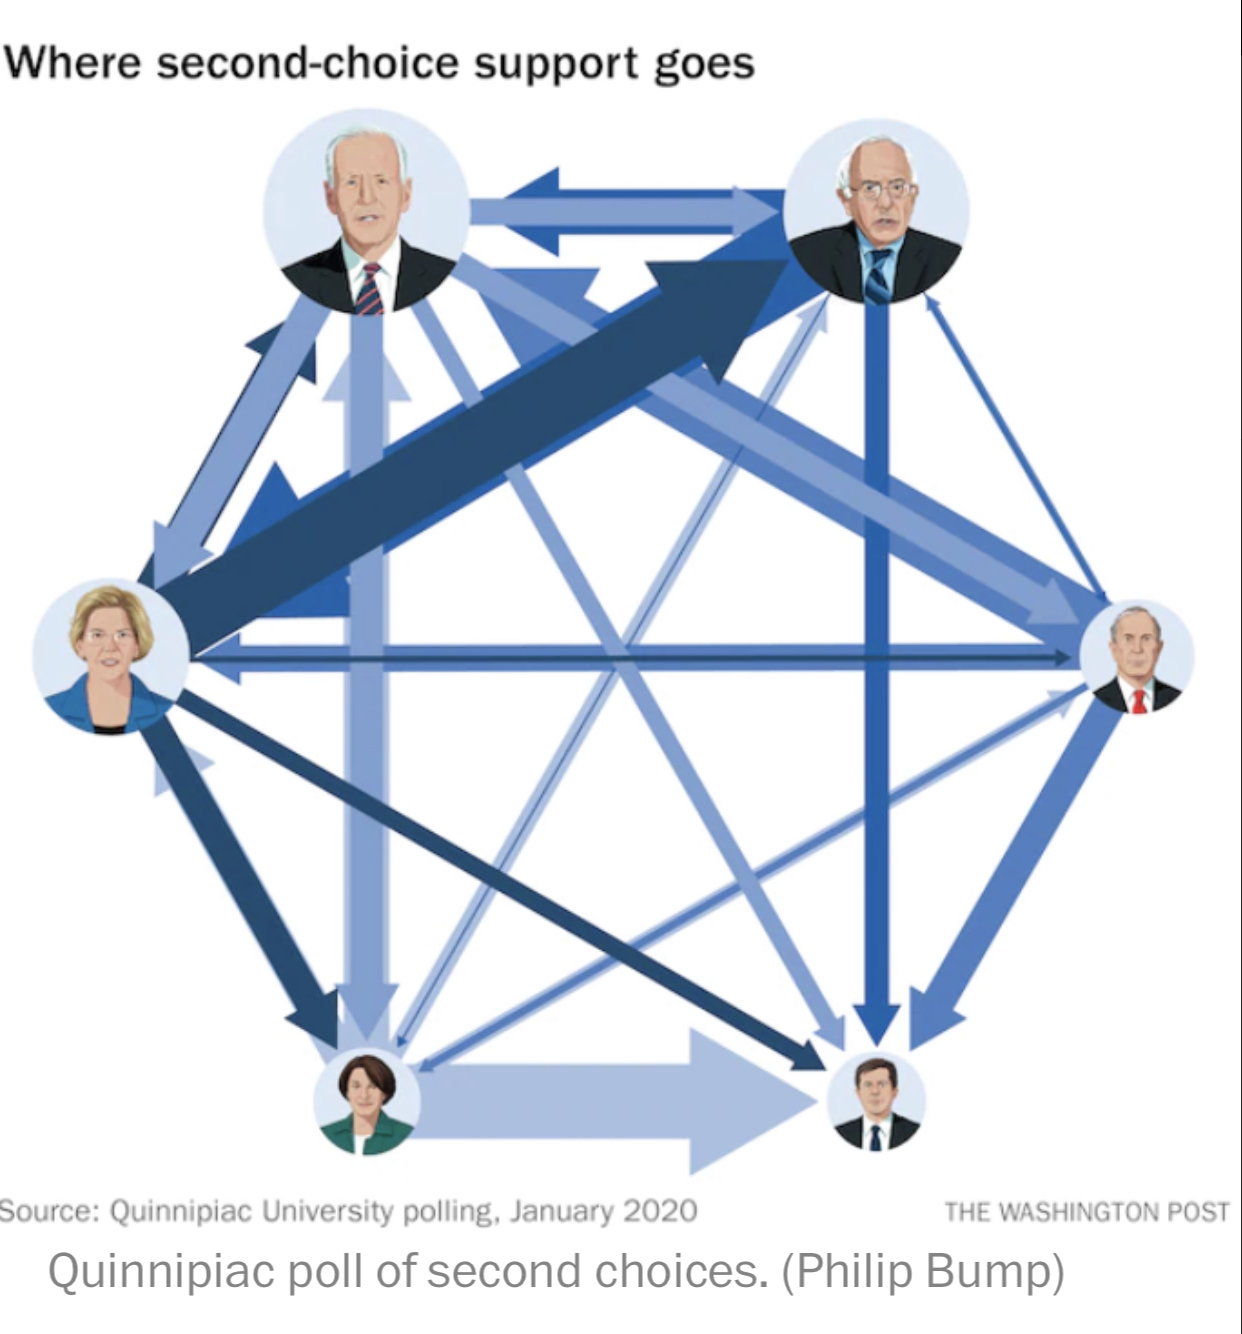
\includegraphics[width=\textwidth]{wapo_second_choices.jpg}}
\only<12>{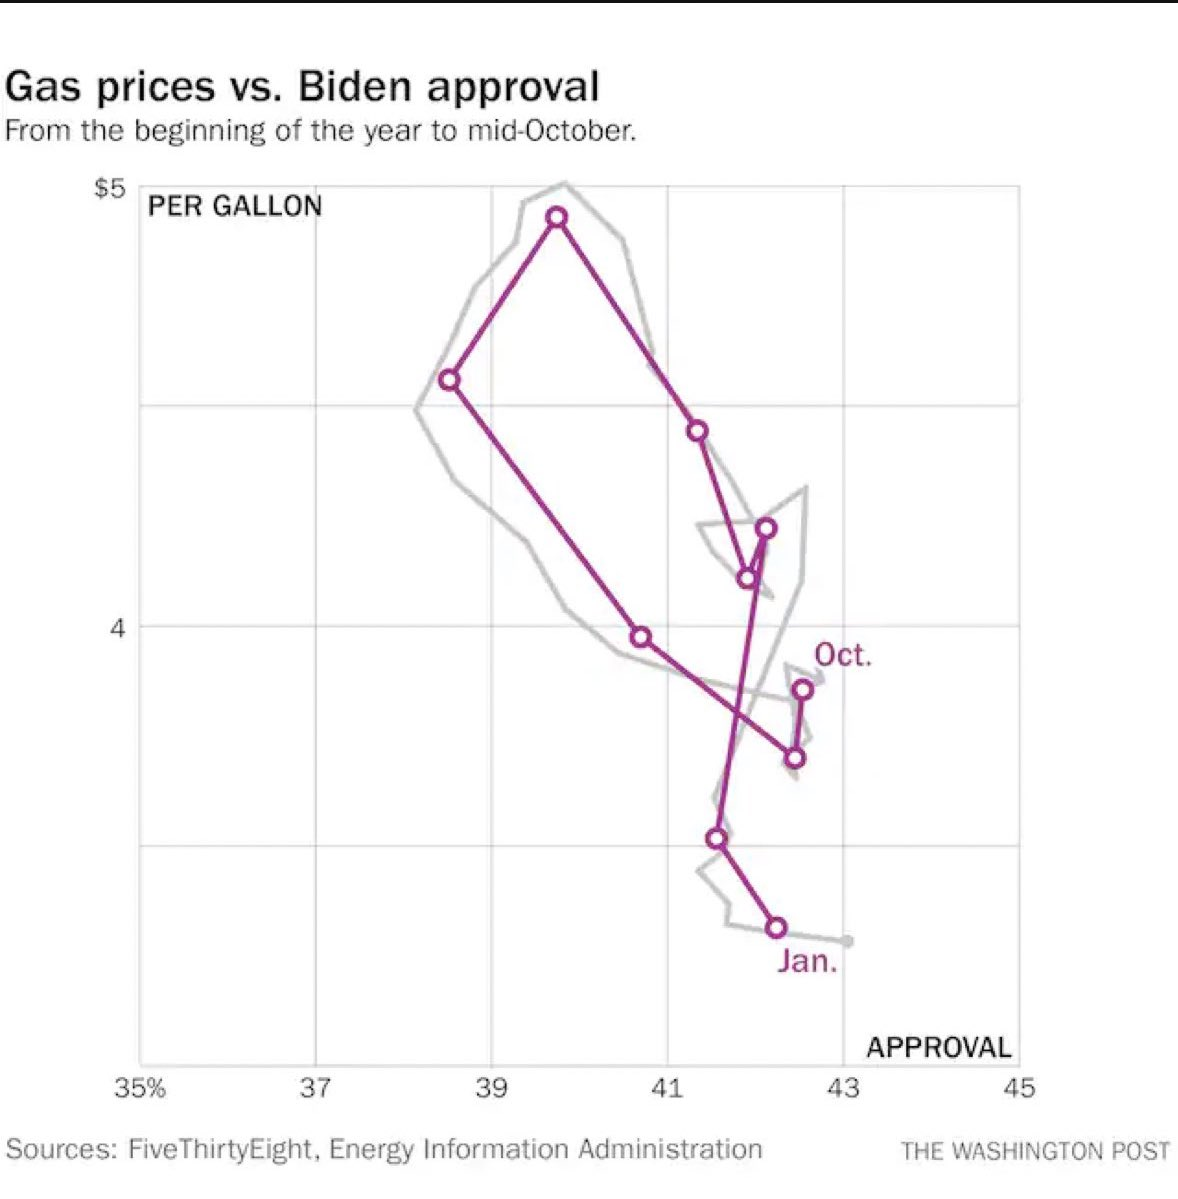
\includegraphics[width=\textwidth]{wapo_gas_prices.JPG}}
\only<13>{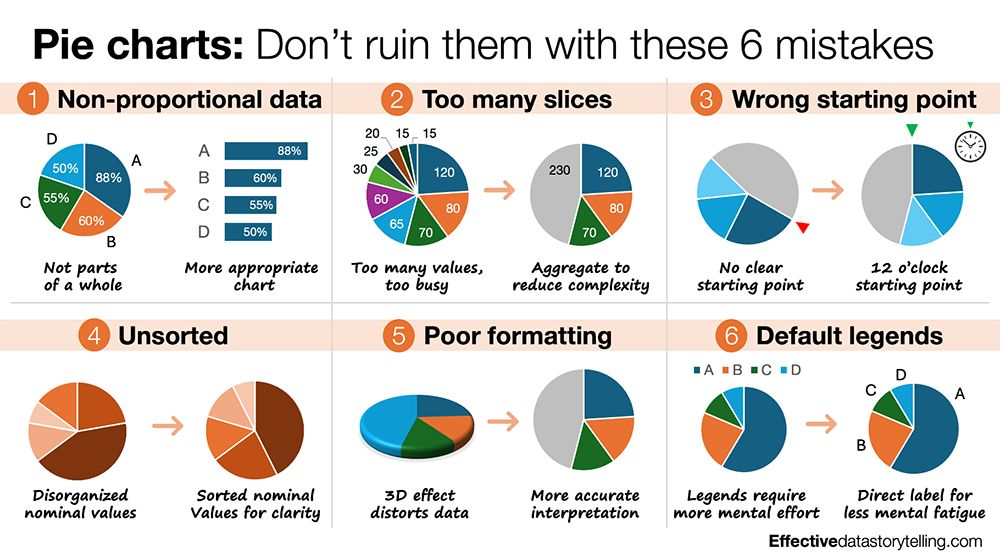
\includegraphics[width=\textwidth]{pie_charts.jpeg}}
\only<14>{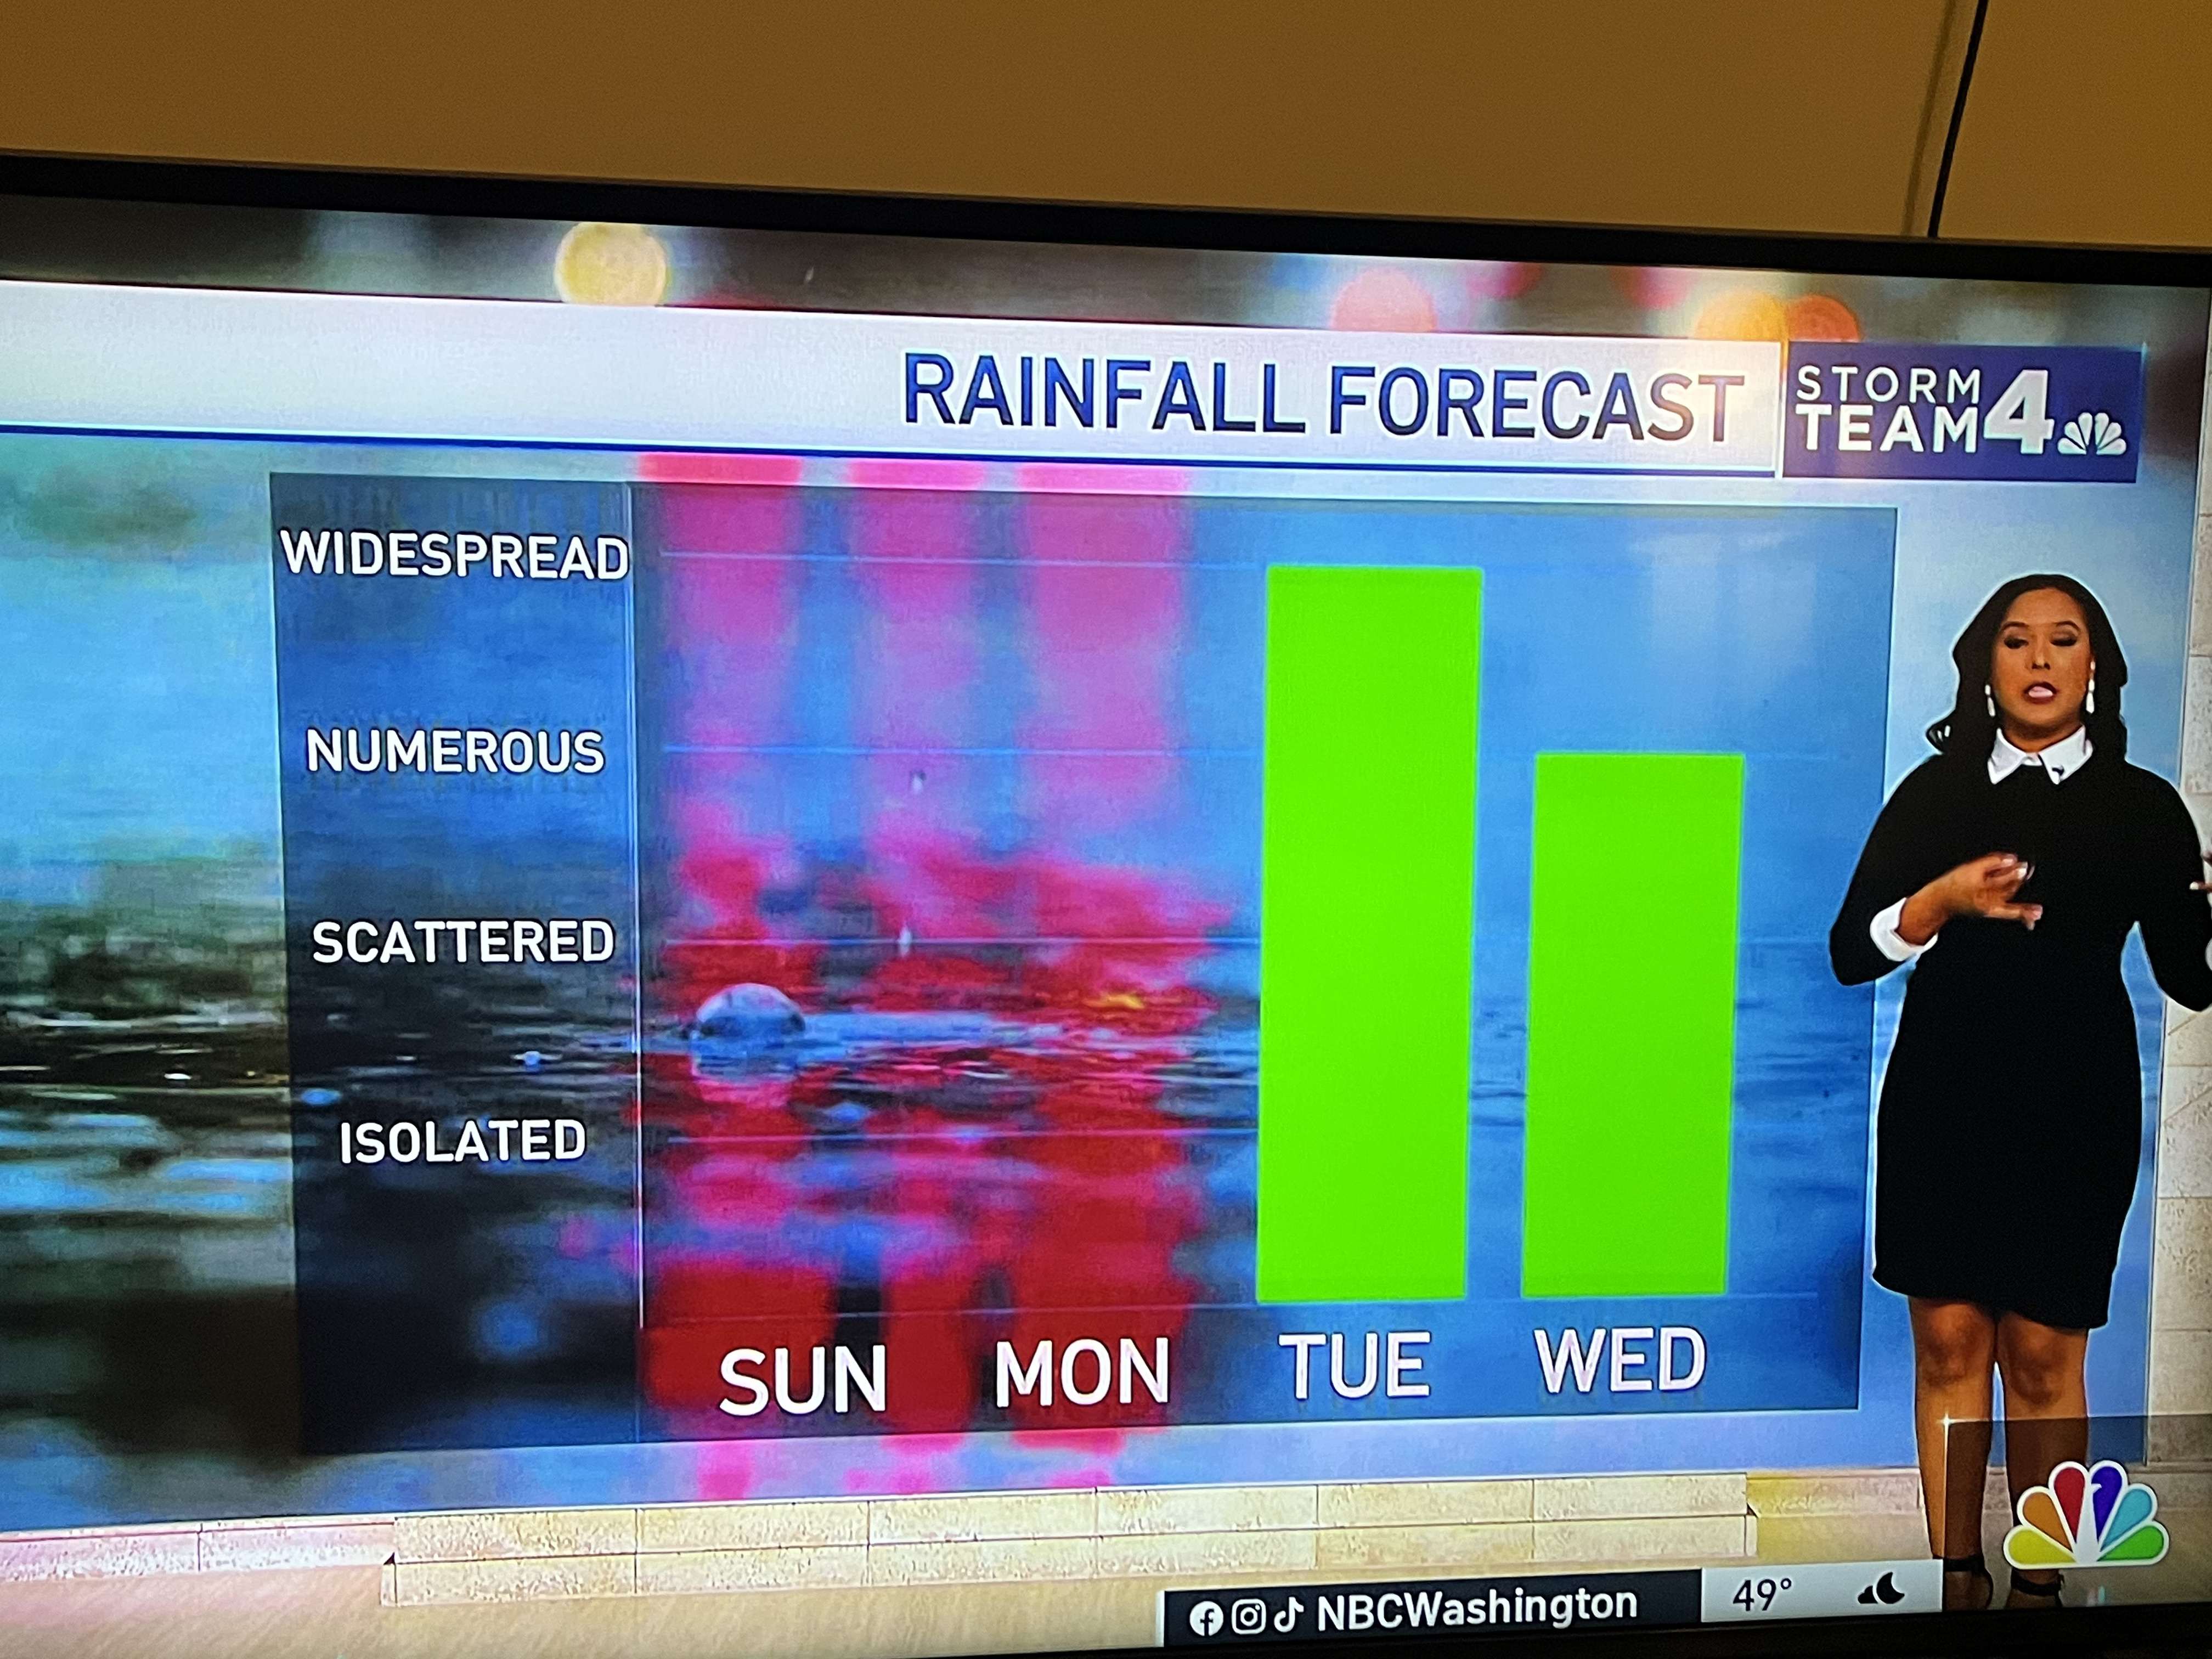
\includegraphics[width=\textwidth]{nbc4_rain.jpg}}
\end{columns}
}

%%%%%%%%%%%%%%%%%%%%%%%%%%%%%%%%%%%%%%%%%%%%%%%%%%%%%%%%%%%%%%%%%%
\frame{\frametitle{Evaluating a Graph}
\begin{columns}
\column{0.4\textwidth}
\begin{enumerate}
    \item Make a note of the first few things you see
    \item Make a note of the first idea that forms in your mind and then search for more
    \item Make notes on likes, dislikes, and wish-I-saws
    \item Find three things you'd change and briefly say why
\end{enumerate}
\column{0.5\textwidth}
\centering
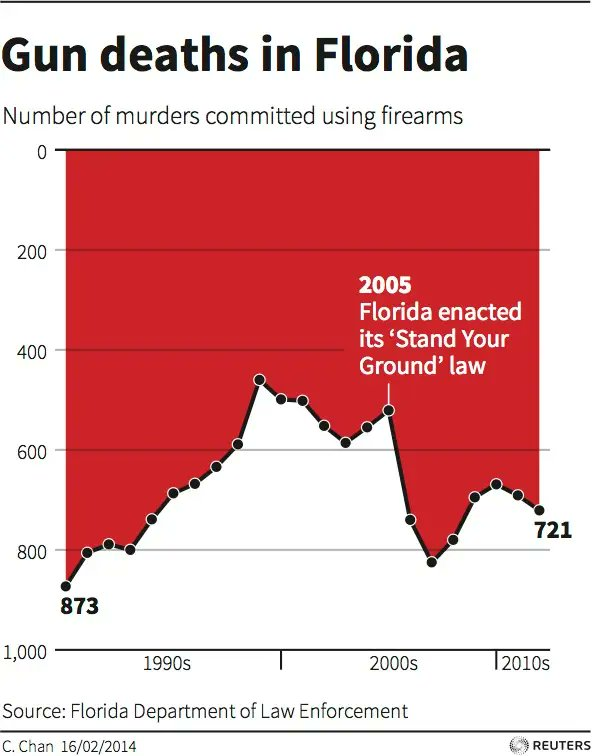
\includegraphics[width=\textwidth]{reuters_guns.JPG}
\end{columns}
}

%%%%%%%%%%%%%%%%%%%%%%%%%%%%%%%%%%%%%%%%%%%%%%%%%%%%%%%%%%%%%%%%%%
\frame{\frametitle{Exercise}
\inserttimer{8}
}

\end{document}
